% An Applied Mathematics/Biology Thesis
% By Jonathan Niles

\documentclass[phd,tocprelim]{thesis}

% escape for previously defined ifpdf
\let\ifpdf\relax

% layout packages
\usepackage{ifpdf}
\usepackage[top=1in, bottom=1in, left=1.5in, right=1in]{geometry}

% font packages
\usepackage{lmodern}
\usepackage{ebgaramond}
\usepackage{amsmath,amssymb,amsthm,mathtools}
\usepackage[T1]{fontenc}

% figure and graphics packages
\usepackage{float}
\usepackage{tabularx}
\usepackage{booktabs,caption,fixltx2e}
\usepackage[flushleft]{threeparttable}
\usepackage{graphicx}
\usepackage{multicol}
\usepackage{caption}

% bibliography, appendix, and reference packages
\usepackage{algorithm2e}
\usepackage{bibentry}
\usepackage{natbib}
\usepackage{appendix}
\usepackage[hidelinks]{hyperref}
\usepackage[toc,nogroupskip,nonumberlist]{glossaries}

%
% Definitions
%
\newtheorem{defn}{Definition}
\newtheorem{thm}{Theorem}
\newtheorem{prop}{Proposition}
\newcommand{\matr}[1]{\mathbf{#1}}
\newcommand*\mean[1]{\overline{#1}}
\newcommand*\conj[1]{\overline{#1}}
\newcommand\addtag{\refstepcounter{equation}\tag{\theequation}}

% make the absolute value command
\DeclarePairedDelimiter\abs{\lvert}{\rvert}%
\DeclarePairedDelimiter\norm{\lVert}{\rVert}%
% Swap the definition of \abs* and \norm*, so that \abs
% and \norm resizes the size of the brackets, and the
% starred version does not.
\makeatletter
\let\oldabs\abs%
\def\abs{\@ifstar{\oldabs}{\oldabs*}}
\let\oldnorm\norm%
\def\norm{\@ifstar{\oldnorm}{\oldnorm*}}
\makeatother

% Set tolerance for box model
\tolerance=9999

% New Commands, refreshers
\renewcommand{\topfraction}{0.85}
\renewcommand{\textfraction}{0.1}
\renewcommand{\floatpagefraction}{0.75}

% Make cornell style
\normalspacing\setcounter{page}{1}\pagenumbering{arabic}
\pagestyle{cornell} \addtolength{\parskip}{0.5\baselineskip}

% LongTabu Fix
\AtBeginEnvironment{longtabu}{\tiny}{}{}   %% change all longtabu content to foot note size

% Make a glossary using the glossaries package
\loadglsentries{./tex/glossary.tex}
\makeglossaries%

% tells bibentry to (re)use the bibliographic data from the standard BibTeX setup by
\nobibliography*

%
% Actual Document Starts here!
%
\begin{document}

% set page numbering to roman for front matter
\renewcommand{\thepage}{\roman{page}}

% import titlepage
% title.tex

\title{Crumble into Cancer: Fragility and Disease in Human Genome Architecture}
\author{Jonathan Niles}
\conferraldate{April}{2015}
\degreefield{Bachelor of Arts}

\maketitle

% acknowledgements.tex

\begin{dedication}
For my grandparents
\end{dedication}

\begin{acknowledgements}
This analysis would not have been possible without the patience, support, and encouragement of my committee members.  I am grateful to
Dr.\ Tyrone Ryba, who took me on as a stranger and worked with me through all my blunders.  Dr.\ Patrick McDonald's advice and
encouragement (though sometimes unheeded) shaped me into a better individual.  Finally, Dr.\ Necmettin Yildirim made my foray into
computation possible through classes, tutorials, and unmatched enthusiasm.  It has been a great honor working with and learning from
each of these great men.

I'd like to thank several other professors who played a formative role in my tuition.  Dr.\ Christopher Hart first interested me in
bioinformatics and taught me programming practices that were invaluable this year.  Dr.\ Amy Clore taught me not only biology, but how
to be a good biologist.

Last but not least, my parents taught me the value of wisdom and work ethic.  If I ever amount to anything, it is a direct product of
their love and support.  Thank you.
\end{acknowledgements}


\contentspage%
\tablelistpage%
\figurelistpage%

\begin{abstract}
Cancer is an enigmatic disease of dysregulation, estimated to cause over half a million deaths in 2015 \citep{siegel2015}.
A patient's prognosis is heavily dependent on the time of detection, fueling research into the origins, biomarkers, and early detection methods for all types of cancers \citep{hirsch2001}.
We hypothesized that the frequency of cancerous lesions in lung cancer cells may be function of morphological changes in genome architecture.  Using human embryonic
stem cells and lung cancer cells, we show that previously discovered topological domains are cell type dependent, and show significant correlation with mutational
frequencies in cancer.  These findings provide motivation for research into the relationships between the dynamic structure of the genome and the propensity to
develop mutations leading to deadly cancers.
\end{abstract}


% set page numbering to arabic for thesis body
\renewcommand{\thepage}{\arabic{page}}

% introduction.tex

\chapter{Introduction}

What causes the genome to break?  The human genome is a six billion nucleotide string that encodes the
the vast instruction set for the cells growth, function, and death.  All possible expression patterns are
encoded in this instruction set, yet particular cell types arise when the instructions are compiled differently
during differentiation.  Modern cancer research indicates the establishment of this epigenetic landscape
determining cell fate may play a strategic role in cancer genesis.

We investigate the mechanical and structural changes during differentiation in order to establish an
architectural link between nuclear topology and the probability of developing cancerous lesions.  We
assume that mutations occurring frequently in specific cancers are based on the epigenetic architecture
of the original cell type.  Using human embryonic stem cells and lung fibroblasts, we propose that
topological changes similar to those that establish patterns of differentiation are responsible for
introducing lesions seen in many cell type specific cancers.

This thesis will proceed as follows.  First, the analytical tools to perform data analysis on genomic
data sets is introduced.  These tools include iterative normalization of chromatin contact maps, eigenvalue
decomposition, and an algorithm to detect topologically associating domains from normalized contact maps.
A literature review of chromatin architecture is presented to provide a strong biological foundation from which
to interpret results.  The methods for data acquisition and processing is described, and we conclude with a
discussion of the results and propose areas of further investigation and improvement.

% math.tex

\chapter{Mathematical Preliminaries}

To extract biologically meaningful information from large data sets, researcher rely heavily on mathematical insights which
guarantee run time estimates, bounds on the problem domain, or interpretation of significance.  While studying the relationship
between chromatin topology and fragility, we leveraged several statistical and linearly algebraic tools.  The following section
will explain the underlying mathematical notions behind the algorithms, the biological rationale, and an interpretation of their
results.  We assume the reader is familiar with the mechanics of linear algebra, an elementary course in statistics, and numerical
analysis.  The reader is heartily encouraged to consult the references to gain a more complete understanding than possible to
present here.

\section*{Normalization of Chromatin Contact Maps}

The entry point for topological analysis begins with a chromatin \gls{contact map}.  The experimental procedure generating a chromatin
contact map, called a Hi-C experiment, is described in detail in Chapter 3.  For now, we will attempt to motivate our
analysis with a simple thought experiment.

Suppose that one wished to record the conformation of a string folded randomly on a surface.  In particular, suppose we focus on intersections
where two strands cross or lie in close proximity.  One possibility would be to place a one-dimensional coordinate system on the string, say
$0 \leq  x \leq  L, x \in \mathbb{N}$.  Since we are interested in overlapping regions, we refer to the region $X_i = \left[ x_{i}, x_{i+1}\right]$
as a bin.  We can record overlapping regions as pairs $(X_i,X_j)$, where position $X_i$ is in close proximity to position $X_j$.  The 
coordinate pairs naturally form a graph, which we represent computationally as a matrix $\matr{O}$.  As $L \rightarrow \infty$, the
resolution of the matrix increases (bin sizes become smaller), and precise interactions on a smaller scale can be differentiated.
Figure~\ref{fig:string} is an example of one such diagram.

\begin{figure}[thb]
  \centering
  \caption{Example: Interactions on a String}
  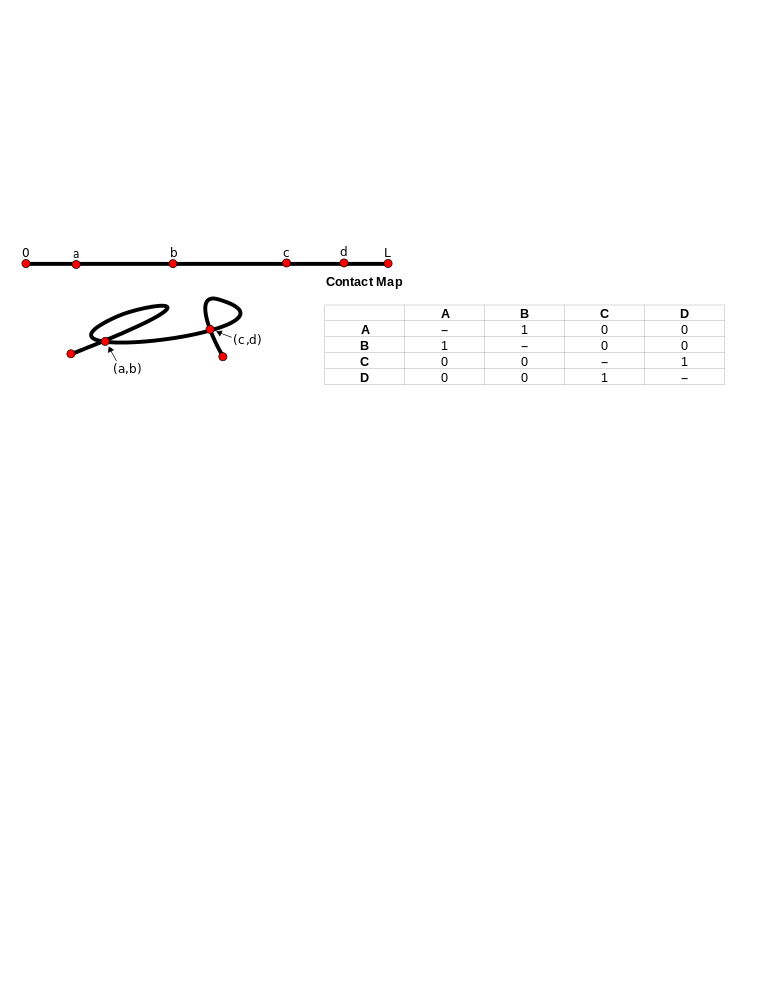
\includegraphics[width=\textwidth]{figures/mathematics/strmtx}\label{fig:string}
\end{figure}

The data structure produced by a Hi-C experiment is identical in spirit to the model developed in our thought experiment.  However, instead of
interactions occurring on a single string, the human genome consists of 24 independent chromosome `strings'.  Furthermore, interaction maps are
generated from populations of cells, yielding millions of copies of each genome.  With this in mind, we propose the following definition:

\begin{defn}
  A chromatin contact map $\matr{O}$ is a symmetric $N \times N$ matrix.  Each cell or bin $O_{ij}$ contains the number of observed contacts
  between regions $i$ and $j$ on the genome.  The contact map is a measure of the contact probability between loci on a genome-wide scale.
\end{defn}

Contacts are recorded by binning the genome into equally sized intervals and considering the pairwise interactions between each bin.
Typically, bins are ordered by increasing genomic coordinates, from the first bin of chromosome 1 to the last bin of chromosome X.
Depending on data quality, bin sizes range from tens of kilobases to megabases.

The critical step of any data analysis pipeline is data \gls{normalization}, which removes experimental biases and noise.  Coupled with quality
control measurements and experimental replicates, normalization also establishes a level of reproducibility.
Several methods exist to normalize contact maps.  Tanay and Yaffe were among the first researchers to undertake a statistical analysis of the
Hi-C experiment in 2011 \citep{yaffe2011}.  They identify several sources of systematic experimental bias in the Hi-C assay and propose a
probabilistic background model that computes the probability of \glspl{trans contact} and \glspl{cis contact} based on regional
\gls{GC} content, fragment length, and genome mappability.  Corrected contact maps are calculated by solving the maximum-likelihood model
parameters on model contact maps, which are then applied to the experimentally derived contact maps.  The mappings
achieved using Tanay and Yaffe's methods provide robust reproducibility between replicates and experiments by considering
\glspl{trans contact} and \glspl{cis contact} separately \citep{yaffe2011}.  This requirement renders their analysis computationally
intensive, prompting further research into simpler methods for Hi-C analysis.

Alternative methods have been developed to normalize contact maps.  Hu and colleagues propose a method `HiCNorm' based on Poisson
regression and achieve a $9000$-fold speed increase compared to Tanay and Yaffe's method \citep{hu2012}.  Recently, Ay and colleagues provide a statistical
method `Fit-Hi-C' that does not assume a particular underlying statistical distribution, instead normalizing \glspl{cis contact} based on probabilistic
analysis of polymer looping dynamics \citep{ay2014}.

Imakaev and colleagues propose a normalization and analysis pipeline \gls{ICE} \citep{imakaev2012}.  We employ \gls{ICE} as the normalization
algorithm in this thesis, due to the availability of its source code\footnote{source: \url{http://mirnylab.bitbucket.org/hiclib/}} and good
performance.  In the following section, we will discuss their algorithm in detail.

\subsection*{\glsentryfull{ICE}}

In pursuit of the true contact probability for each genomic region, \gls{ICE} makes a critical observation that the bias matrices determined by
Yaffe and Tanay \citep{yaffe2011} can be successfully reproduced ($r = 0.99$) as a product of biases $B_i \times B_j$.  This observation leads
immediately to the following proposition

\begin{prop}
  Given the assumption of factorizable biases, the expected contact frequency $\varepsilon_{ij}$ for every pair of regions $(i,j)$ can
  be written as $\varepsilon_{ij} = B_{i}B_{j}T_{ij}$, where $B_i$ and $B_j$ are biases and $T_{ij}$ is the sought matrix of relative contact
  probabilities, normalized as $\sum_{i, i \neq j, j \pm 1}T_{ij} = 1$.  The normalized contact map is give as
  $T_{ij} = \frac{\varepsilon_{ij}}{B_{i}B_{j}}$.
\end{prop}

The authors note that this normalization procedure results in `equal visibility' regions across the entire genome and maps which are
comparable between Hi-C data sets.  They propose the following algorithm to obtain the biases $B_i$ and `true' relative contact probabilities
$T_{ij}$.

\begin{algorithm}[H]
  \KwData{A matrix of observed interactions $O_{ij}$}
  \KwResult{A matrix of relative contact probabilities $T_{ij}$ and bias vector $B_i$}
  Initialize $W^{0}_{ij} = raw contact matrix$; $B^0 = 1$; $k = 1$\;
  \While{$\abs{B^{k+1} - B^{k}} < \delta$}{%
    $S_i = \sum_{j}W^{k}_{ij}$\;
    $\mean{S_i} = \frac{1}{n}\sum_{i = 1}^{n}S_i$\;
    $\Delta{}B^k_i = \frac{S_i}{\mean{S_i}}$\;
    $W^{k+1}_{ij} = \frac{W^k_{ij}}{\Delta{}B^k_i\Delta{}B^k_j}$\;
    $B^{k+1}_i = B^k_i \dot \Delta{}B^k_i$\;
    $k = k + 1$\;
  }
  \caption{Iterative Correction}
\end{algorithm}

It is not apparent that this algorithm is correct or even converges.  To gain an intuitive understanding of the solution, let us investigate a
simpler proposition.  Suppose that, instead of defining $O_{ij}$ to be the matrix product $B_{i}B_{j}T_{ij}$, we consider the counts
in $O_{ij}$ are the expectation of some multinomially distributed random variable $X_{ij}$, where $E[X_{ij}] = NB_{i}B_j$ for some
constant $N$ and vector $B$ whose cumulative sum is 1 ($\sum_{i}B_i = 1$).  In this formulation, we relax our criteria such that each cell
$O_{ij}$ is independent and distributed according to $B$.  The count of cell $i,j$ is given by the probability

\begin{align}
  \label{eqn:probmodel}
  \begin{split}
    p_{ij} &= NB_{i}B_{j}
    \\
    \log{p_{ij}} &=  c + u_i + u_j - Z
  \end{split}
\end{align}

where $c = \log{N}, u_i = \log{B_i}, u_j = \log{B_j}$, and $Z (= c)$ is a normalization factor to ensure that $\sum p = 1$.  This type of
model is called a \gls{log-linear} or \gls{toric model}.  $p$ is an observation from some distribution $p \sim \mathcal{f}(X)$.  The challenge to
parameterize the model and fit the model to the observed map.  The problem one of \gls{MLE}: what are the maximum likelihood parameters
that best fit the model to the observed data?  Fortunately, methods and their convergence properties for solving \glspl{MLE} have been extensively
studied in the literature \citep{fienberg2012, pachter2005}.

% TODO
In the realm of statistics, the contact matrix, together the vector sums of the rows and columns (margins), is called a \gls{contingency table}.  Assuming
that the margins are positive, and that the matrix cannot be permuted into block diagonal shape, Birch's theorem guarantees that there is a
unique maximum to the likelihood function \citep{pachter2005,bishop1975}.  For full details, consult Discrete Multivariate Analysis by
Bishop \citep{bishop1975}.  Furthermore, the marginal values are the \glspl{sufficient statistic} of the model.  In other words, the maximum
likelihood parameters for this data is given by the normalized row and column sums of the matrix \citep{pachter2005}.

With the observation that there exists a global maximum of the likelihood function, all that remains is to compute the true values by some
process.  One common algorithm is the \gls{EM} algorithm \citep{fuchs1982}.  Imakaev and colleagues employ a simpler algorithm known as \gls{IPF},
developed by Deming and Stephan in 1940, and apparently rediscovered by Imakaev's group \citep{deming1940}.  \gls{IPF} works generally by solving
the \gls{MLE} problem while leaving the margins ($p_{i+} = \sum_{j}p_{ij}$ and $p_{j+} = \sum_{i}p_{ij}$) fixed.  A proof of convergence for contingency
tables follows from Fienberg's work in algebraic geometry in 1970 \citep{fienberg1970}. %TODO explain feinburg more

Finally, we return to the \gls{toric model} we described in Eqn.~\eqref{eqn:probmodel}.  Since the log-likelihood function is concave, the \gls{IPF} algorithm first
computes the roots of the partial derivatives of the log-likelihood function and sets them to zero to solve for the global maximum.  Imakaev
and colleagues consider the likelihood function on the Poisson distribution, given by the \gls{pdf} $f(O;E) = \frac{E^{O}}{O!e^{-E}}$.  The
log-likelihood function for the Poisson distribution is given

\begin{align}
  \label{eqn:llmodel}
  LL = \sum_{ij}\left[O_{ij}\log{(T_{ij}B_{i}B_{j})} - T_{ij}B_{i}B_{j} - \log{(O_{ij}!)}\right]
\end{align}

Differentiating with respect to $T_{lm}$ and $B_m$ and setting the derivatives to zero yields

\begin{multicols}{2}
  \begin{align}
    \label{eqn:modelderivative1}
    \begin{split}
      \frac{dLL}{d\matr{T}_{lm}} = \frac{O_{lm}}{T_{lm}} - B_{l}B_{m} = 0
      //
      \frac{dLL}{dB_{m}} = \sum_i\left[\frac{\matr{O}_{im}}{B_m} - T_{im}B_i\right] = 0
    \end{split}
  \end{align}

  \break%

  \begin{align}
    \label{eqn:modelderivative2}
    \begin{split}
      T_{lm} = \frac{\matr{O}_{lm}}{B_{l}B_{m}}
      \\
      \sum_i\left[\frac{\matr{O}_{ij}}{B_{m}B_{i}} - \matr{T}_{im}\right]
    \end{split}
  \end{align}
\end{multicols}

It is clear that Eqn.~\eqref{eqn:modelderivative2} is satisfied if a solution is found for Eqn.~\eqref{eqn:modelderivative1}.  Taking the first equation together  with the
normalization $T_{ij}$ yields

\begin{align}
  \label{eqn:result}
  \sum_i \frac{\matr{O}_{ij}}{B_{i}B_{j}} = 1
\end{align}

A similar process yields that a broad class of distributions give the same result \citep{imakaev2012}.

\section*{Principal Component Analysis}

The holy grail of data analysis on high-dimensional data is dimensionality reduction --- that is, to find an accurate representation of
the experiment that need not invoke all the dimensions measured.  This is often performed as a preprocessing step to increase storage capacity
and algorithm speed.  Since experiments such as Hi-C produce data on large numbers of features, researchers must find ways to remove redundancy,
eliminate unneeded parameters and compress data sets.  One of the most popular methods is called \gls{PCA} \citep{law1987}.

Data in high dimensions are difficult to visualize and interpret.  Two common questions in data analysis are `what changed?' and `what
remained the same?' between measurements.  \gls{PCA} answers these questions by finding a representation of the data that maximizes
the \gls{variance} or variation between observations in the data set.  The output of \gls{PCA} is a transformed data set on a new coordinate
system, called components.  The \glspl{PC} are a subset of these components that capture `most' of the variation in the data set.  The researcher
must compare the calculated components to the original data set and determine which variables, or combination thereof, the components represent.

\begin{defn}[Principal Component Analysis]
  A statistical procedure that transforms a number of possibly correlated variables into a smaller number of uncorrelated variables.
\end{defn}

In practice, there are two methods used for \gls{PCA}.  The simplest to explain, but more error-prone, is the eigen-decomposition
method \citep{smith2006}.  In this procedure, for a data matrix $\matr{A}$, the eigenvalues of the covariance matrix $\matr{A}\matr{A}^T$
are computed directly as the principal components.  However, since this method requires an extra matrix multiplication, numerical
errors are more likely to be introduced during large computations. In practice, \gls{PCA} often derived in conjunction with \gls{SVD}
and we will hold to that standard here.

\begin{thm}[Singular Value Decomposition]
  Let $\matr{A} \in M_{n}(\mathbb{R})$ be given. Then there are unitary matrices $\matr{V} \in M_n$ and $\matr{W} \in M_n$, and a square diagonal
  matrix
  \[
    \matr{\Sigma} =
      \begin{bmatrix}
        \sigma_1 &        & 0        \\
                 & \ddots &          \\
        0        &        & \sigma_n \\
      \end{bmatrix}
  \]
  such that $\sigma_1 \geq \sigma_2 \geq \cdots \geq \sigma_n$ and $\matr{A} = \matr{V}\matr{\Sigma}\matr{W}^*$.  The parameters $\sigma_1$,
  $\hdots$, $\sigma_n$ are the positive square roots of the decreasingly ordered non-zero eigenvalues of $\matr{A}\matr{A}^*$, which are the
  same as the decreasingly ordered nonzero eigenvalues of $\matr{A}^*\matr{A}$.
\end{thm}

To prove that any square matrix $\matr{A} \in M_n(\mathbb{R})$ can be decomposed into singular values, we will use some matrix definitions. The
reader is reminded of the definitions of \textit{normal} $(\matr{A}\matr{A}^* = \matr{A}^*\matr{A})$, \textit{Hermetian} $(\matr{A}^* =  \matr{A})$,
and \textit{unitary} $(\matr{A}^*\matr{A} = \matr{A}\matr{A}^* = 1)$ matrices.  Further, two matrices $\matr{A}, \matr{B} \in M_n$ are said to be
\textit{unitarily similar} they are similar by a unitary matrix $(\matr{A} = \matr{U}\matr{B}\matr{U}^*)$.  We are now ready to begin the proof.

\begin{proof}[Singular Value Decomposition]
  It should be clear the matrices $\matr{A}\matr{A}^* \in M_n$ and $\matr{A}^*\matr{A} \in M_n$ have the same eigenvalues, and hence, they are
  unitarily similar.  Then there exists a unitary matrix $\matr{U}$ such that $\matr{A}^*\matr{A} = \matr{U}(\matr{A}\matr{A}^*)\matr{U}^*$.  Then

  \[
    {(\matr{UA})}^*(\matr{UA}) =
    \matr{A}^*\matr{U}^*\matr{UA} =
    \matr{A}^*\matr{A} =
    \matr{UA}\matr{A}^*\matr{U}^* =
    \matr{UA}{(\matr{U}\matr{A})}^*
  \]

  so $\matr{UA}$ is normal.  Let $\lambda_1 = \abs{\lambda_1}e^{i\theta_1}, \ldots, \lambda_n = \abs{\lambda_n}e^{i\theta_n}$ be the positive eigenvalues of
  $\matr{UA}$ in decreasing order.  Furthermore, let $\Delta = diag(\lambda_1, \ldots, \lambda_n)$, let $D = diag(e^{i\theta_1}, \ldots, e^{i\theta_n})$,
  let $\Sigma = diag(\abs{\lambda_1}, \ldots, \abs{\lambda_n})$, and let $\matr{X}$ be a unitary matrix such that $\matr{UA} = \matr{X\Delta}\matr{X}^*$.  Then
  $D$ is unitary and

  \[
    \matr{A} = \matr{U}^*\matr{X}\Sigma\matr{D}\matr{X}^* = (\matr{U}^*\matr{X})\Sigma(\matr{D}\matr{X}^*)
  \]

  If we denote $\matr{V} = \matr{U}^*\matr{X}$ and $\matr{W} = \matr{X}\matr{D}^*$, we have our desired factorization, and
  $\sigma_j = \abs{\lambda_j}, j = 1, \ldots, n$.
\end{proof}

A full proof of \gls{SVD} for rectangular matrices can be found in Horn and Johnson \citep{horn2013}. The relationship between
\gls{SVD} and \gls{PCA} follows directly from the definition of \gls{SVD}.

\begin{thm}
  Let $\matr{A} = \matr{V}\matr{\Sigma}\matr{W}^*$ be the \gls{SVD} of an $n \times n$ dimensional matrix $\matr{A}$ and let

  \[
    \matr{C} = \frac{1}{n - 1}\matr{A}^*\matr{A}
  \]

  be the covariance matrix.  The eigenvectors of $\matr{C}$ are the same as the \textnormal{right singular vectors} of
  $\matr{\Sigma}$.
\end{thm}

\begin{proof}
  Compute
  \[
    \matr{A}^*\matr{A} =
    \matr{V\Sigma}\matr{W}^*\matr{W\Sigma}\matr{V}^* =
    \matr{V\Sigma\Sigma}\matr{V}^* =
    \matr{V}\matr{\Sigma}^2\matr{V}^*
  \]

  \[
    \matr{C} = \matr{V}\frac{\matr{\Sigma}^2}{n - 1}\matr{V}^*
  \]

  $\matr{C}$ is symmetric, and unitarily diagnolizable.  Hence, the eigenvectors of the covariance matrix $\matr{C}$ are the same as the
  matrix $\matr{V}$ (right singular vectors) and the eigenvalues of $\matr{C}$ can be computed directly from the singular values
  $\lambda_i = \frac{\sigma_i}{n - 1}$.
\end{proof}

The ordered eigenvectors are the \glspl{PC} we desire.  In exploratory data analysis, the variance captured by each \gls{PC} is found
by analyzing the relative sizes of the positive eigenvalues, typically in the form of a scree plot.  In the Hi-C capture experiment, Dekker
and colleagues \citep{dekker2012} focus on the component that captures genome `compartment character', the banding pattern of interactions
observed on Hi-C maps, regardless of captured variance.  In our case, the \gls{PCA} decomposition provides a measure of compartment character
for a given bin on the Hi-C map.

\section*{Detecting changes in local chromatin interaction}

\gls{PCA} is a useful technique for identifying gross differences between data sets.  For subtle changes of local chromatin structure, we appropriate a
technique developed by Dixon and colleagues \citep{dixon2012}, termed the \gls{DI}.  Intuitively, the \gls{DI} for a given region of chromatin gives the
relative `upstream' or `downstream' character of the interactions involving that particular chromatin region.

The basic premise of the \gls{DI} algorithm is simple.  For each bin along the genome, we calculate the number of upstream and downstream interactions and
assign the normalized difference ($downstream - upstream$) as the \gls{DI} for that particular bin.  The index captures the downstream or upstream bias of
a genomic region. The formulation of the directionality index is given in the supplementary methods of Dixon's paper  \citep{dixon2012}

\begin{align}
  \label{eqn:di}
  DI = \left(\frac{B - A}{\abs{B - A}}\right)\left(\frac{{(A - E)}^2}{E} + \frac{{(B - E)}^2}{E}\right)
\end{align}

where $A$ is the number of upstream reads in a given window, $B$ is the number of downstream reads, and $E$ is the expected number of interactions under
the null distribution ($\frac{A + B}{2}$).  Dixon and colleagues apply the directionality index to examine 2Mb windows upstream and downstream on a
normalized 40kb resolution contact map.  From the \gls{DI} vector, they employ a \gls{HMM} to discover X domains with prominent upstream and downstream bias.
They concluded that these domains were (not) conserved across cell types, but may represent an underlying regulatory structure in particular cell or tissue
types \citep{dixon2012}.

% bio.tex

\chapter{Biological Preliminaries}

\section*{Introduction}

Even if limited in scope to genome architecture, a satisfactory discussion relating cell state and architectural regulation would fill
volumes.  In the following chapter, we will discuss the topics and recent developments from genetics and molecular biology that most
directly relate to chromatin architecture and the implications of a shifting interaction map.  Readers are strongly encouraged
to consult a molecular biology text, such as Molecular Biology of the Cell \citep{alberts2002}, for a rich discussion of mechanism
regulating cell state and function.

The sheer complexity of the nucleus is best decomposed into a structural hierarchy with several layers of granularity: the primary
sequence of \gls{DNA} base pairs, architectural modeling proteins, transcription factors and other binding proteins, and \glspl{CT}
and other macro molecular chromatin structures.  Within these categories there are deeper layers of regulation, such as nested
organization of topological domains or alternative splicing in transcription.  Conformational changes at smaller resolutions generally
invoke targeted, local events, while genome-wide conformation shifts enable regulation on whole cell level.  This conceptual hierarchy
is useful to keep in mind when investigating the origin of gene expression changes, differentiation, or disease states.  We will
consider each of these levels in sequence.

\section*{The Nuclear Hierarchy}

It is difficult to overstate the importance of chromatin topology.  The morass of nucleic acids and proteins packed tightly inside the
nuclear envelope somehow contain all the information required for cell function and proliferation.  The central dogma of molecular biology,
outlined in the notes of Francis Crick's `Ideas on Protein Synthesis' \citep{crick1970} illustrates how information flows from primary
sequence through protein.  The central dogma therefore strongly reinforces the importance of \gls{DNA} content, readability, and expression.

\begin{figure}[b]
  \centering
  \caption{The original central dogma of molecular biology \citep{crick1970}}
  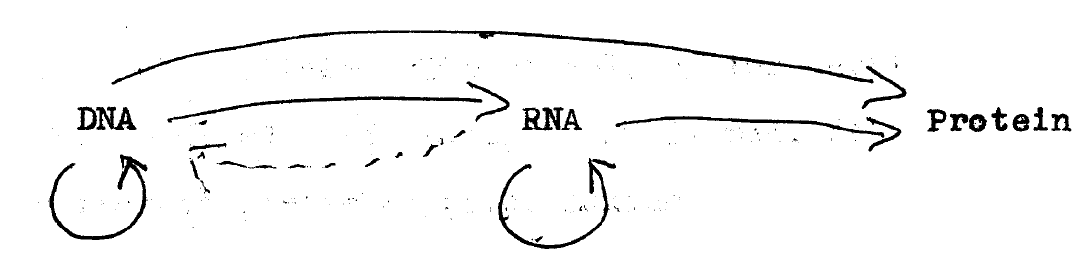
\includegraphics[width=\textwidth]{figures/biology/dogma}\label{fig:dogma}
\end{figure}

\subsection*{The Primary Sequence}

The fundamental informational unit of the cell is the \gls{nucleotide}, often called a nucleotide base or \gls{bp} when joined in a
\gls{DNA} molecule or strand.  Eukaryotic cells have a principal four character alphabet of nucleotides, distinguished by their \glspl{nucleobase}:
adenine, cytosine, guanine, and thymine.  Nucleotides are affixed to a phosphate backbone in a long, coiling polymer chain, called \gls{DNA}.  The
famous publication of the structure of \gls{DNA} in 1953 by researchers James Watson and Francis Crick demonstrates these polymers
exist in the nucleus as double helices \citep{watson1953}.  Strong hydrogen bonds between opposing nucleotides hold the double helix together
in solution.  Nucleotides are classified based on the chemical structure of there nucleobase into purine or pyridine bases; adenine and guanine are purine bases,
while thymine and cytosine are pyridine bases.  \gls{DNA} bonds form between complementary nucleotides from opposite groups: adenine and thymine form
two hydrogen bonds and guanine and cytosine form three hydrogen bonds between their bases.  Thus, one half of the helix completely
determines the other half and perturbations of this structure may lead to strand mutations \citep{alberts2002,cox2008}.

One cannot ignore the constituents of the primary sequence, particularly when considering macroscopic properties of the genome.  The nucleotide content and
order affects local sequence flexibility directly (by encoding binding sites) or indirectly (by supporting the binding of histones), and
modulates the binding of important architectural proteins \citep{travers2004}.  Although a \gls{DNA} strand is a helical structure, it is an intrinsically
flexible molecule.  A naive calculation reveals that the human genome is roughly two meters in length%
\footnote{%
  A diploid human genome consists of two copies of the $\sim3.1Gb$ DNA molecule, based off estimates from the \gls{NCBI} human genome reference build 37.
  Each base pair is assumed to be roughly $0.34\times10^{-9}m$.  The entire length is $2(0.34 \times 10^{-9})(3.2 \times 10^9) = 2.176m$.
},
yet the entire genome fits into a nuclear volume of $\sim523\mu$m \citep{marks2011}.  Loops as small as 100 bases in length have been
reported in enhancer and repressor element activation pathways \citep{wong2008}.  Furthermore, These loops can form independently of proteins
\citep{vafabakhsh2012}, indicating these loops do not impose excessive torsional strain.  Altogether, \gls{DNA}'s inherent flexibility furnishes the
foundation for complex higher order chromatin structures.

\gls{DNA} bases can also be directly modified by binding additional biochemical groups.  Cytosine undergoes \gls{DNA} methylation, also called GC methylation
to distinguish it from a histone modification of the same name \citep{bird2002}.  Methylation is an important epigenetic mark, involved in imprinting,
\gls{X-inactivation}, and maintaining heritable epigenetic states \citep{law2010}.  In mammals, \gls{DNA} methylation occurs almost exclusively along
symmetric \gls{GC} dinucleotides, and is estimated to occur at $\sim70-80\%$ of the \gls{GC} sites throughout the genome \citep{ehrlich1982,law2010}.
In the context of global chromatin architecture, \gls{DNA} methylation is thought to change chromatin conformation by recruiting histone
de-acetylaces \citep{schubeler2000}, suppressing large domains as in X-inactivation, recruiting architectural proteins directly \citep{yu2000},
and inhibiting transcription \citep{kass1997}.

\subsection*{Epigenetics And Chromatin Modeling}

How a \gls{DNA} molecule is packaged and condensed within a cell nucleus remains one of the basic questions of cell biology.  Intellectual curiosity aside,
why is it so important to unravel the chromosomal architecture?  Researcher J.C. Hansen notes, `In biology, structure is inexorably linked to function.' \citep{hansen2012}
The pursuit of an accurate \textit{\gls{in vivo}} model for \gls{DNA} and protein packaging continues to persist today, despite a legacy of experimental,
conceptual, and mathematical models.

In 1974, Kornberg discovered that chromatin contained roughly equal amounts of \gls{DNA} and protein \citep{kornberg1974}.  A year later, \citet{oudet1975}
and colleagues described the separation of chromatin into protein complexes spaced evenly on the \gls{DNA} molecule as `beads on a string' \citep{oudet1975}.
The observed beads are nucleosomes, bundles composed of a histone octamer and $\sim200$ bases (later reported to be $167$ bases) \citep{robinson2006} of
coiled \gls{DNA}. Much as the nucleotide is the fundamental unit of the genome, nucleosomes are the fundamental units of the epigenome.  Nucleosomes in
series are called a \gls{nucleosome array}.  A nucleosome consists of two components: a core particle wrapping $\sim146$ base pairs of DNA, yielding a
6 fold compaction in length, and a linker portion of varying length of $0$ to $\sim80$ base pairs.  The linker component connects adjacent nucleosomes
in a nucleosome array \citep{wu2007, hansen2012}.  These arrays are $10-nm$ in diameter, provoking them to be often called the `$10-nm$' fibers.

Despite decades of research on nucleosome arrays, their structural conformation \textit{\gls{in vivo}} remains enigmatic.  Does a higher order structure
between the $10-nm$ fiber and mitotic chromosome exist?  Nucleosome arrays and linker histones suspended in ionic solution fold naturally into a $30-nm$ fiber
\citep{tremethick2007}; however, it is unclear whether this motif forms \textit{\gls{in vivo}} and its conformation may be different in the nuclear context \citep{bian2012}.
The $30-nm$ fiber model is appealing as it readily explains the highly compacted structure of mitotic chromosomes.  To form the fiber, arrays of nucleosomes
are arranged in a solenoid or double-helix structure (for full review, see Grigoryev and Woodcock \citep{grigoryev2012}).  Whether one or both structures
are present in sub-chromosomal architectures is still an open question \citep{song2014}.  Recently, experiments using cryogenic electron microscopy
(cryo-EM) suggested an alternative fractal arrangement of $10-nm$ fibers, without invoking a higher organizational unit \citep{nishino2012,hansen2012}.
It is likely that a mixture of these organizational schemas exist in the cell.  Further research is needed to assess the biological relevance of the $30-nm$ fiber in
both interphase and mitotic chromosome structure.

The nucleosome core particle is a central actor controlling gene expression through local transcription regulation.  It is well established that nucleosomes
cause an attenuation of gene expression when present at physiological concentrations \citep{brown1984, lorch1987,laybourn1991,juan1994}. How
then does the cell maintain some genes as actively transcribed while others are silenced?  Nucleosomes regulate gene expression by regulating accessibility.
Gene expression is mediated by a confluence of protein-DNA interactions: enhancers bind to enhancer elements, polymerases to the \gls{TSS}, and polymerase
recruitment proteins line the promoter region to facilitate polymerase binding and transcription activation \citep{cox2008}.  At any protein-DNA junction,
local chromatin compaction can exclude binding by physically restricting access to the primary sequence.  This tightly packed form of DNA is called
\textit{\gls{heterochromatin}}, while open and accessible sequence is called \textit{\gls{euchromatin}}.

A critical component of gene regulation is the ability to form long range interactions between distal elements of the genome.  Enhancer or silencer elements
situated at great distances (hundreds of kilobases) from a gene promoter will form loops in the chromatin to situate that element near the target
promoter \citep{heintzman2007}.  The commonly-held view is that there are three distinctive classes of proteins facilitating gene transcription: \glspl{GTF},
promoter-specific activators, and coactivators.  \glspl{GTF} form on the promoter region, to form a \gls{PIC}, called the \gls{core promoter}.  While the
\gls{core promoter} assembly is enough to detect a basal level of transcription, often activators, proteins bound to regulatory regions upstream, downstream,
or even in neighboring genes, are recruited to the promoter region to facilitate greater level of transcription, forming long chromatin loops \citep{ptashne1997}.
Coactivators function as intermediaries in the assembly of the promoter complexes, binding both the activators and the \gls{PIC} to achieve faster throughput of
gene expression.

\subsection*{Chromosomes are organized in territories}

The highest level of genome organization is the \gls{CT} or chromosome neighborhood \citep{cremer2001}.  The hypothesis that chromosomes are segregated into
nuclear sub-volumes dates back more than 100 years \citep{cremer1993}.  The raison d'etre for these territories is not well understood; however, it is proposed
that \gls{CT} distribution in the nucleus protects the gene-rich chromosomes by localizing them to the nuclear center \citep{boyle2001, federico2006}.
\glspl{CT} create gene expression `pockets' with localized transcriptional and repair machinery \citep{bolzer2005}, and may have cell type specific positioning.

To date, there is no evidence to support a deterministic ordering of chromosomes in the nucleus.  However, there may exist certain deterministic rules to
chromosomal positioning.  In all human cell types studied, the radial position of the chromosomes is correlated with gene density and chromosome
size \citep{sun2000,bolzer2005}.  In most cell types, gene-rich chromosomes are found in the central nuclear compartment, while gene-poor
chromosomes surround the nuclear periphery, most likely to protect actively transcribed genes from mutagens that may invade the nucleus \citep{boyle2001,kozubek2005}.
However, in cell types with non-spherical nuclear shapes, chromosomal arrangements may deviate from this pattern, possibly reflecting more
specialized functions \citep{bolzer2005}.

There is strong evidence that chromosomal territories contain small decondensed regions serving as gene expression hot-spots.  Unlike bacterial chromosomes,
in which genes from the same pathway are grouped on the chromosome in units called \textit{\glspl{operon}}, eukaryotic genes are distributed seemingly randomly
throughout the genome \citep{jacob1961}.  It is well known that transcriptionally active chromatin compartmentalizes based on replication
timing \citep{ferreira1997,sadoni1999,thevenin2014}.  Moreover, recent observations reveal in order to facilitate transcription of genes in
a pathway, chromosomal territories co-localize functionally related genes with transcriptional machinery.  When considering only inter-chromosomal gene
pairs, Thevenin and colleagues observed that co-functioning genes exhibit significant local concentrations, regardless of linear distance on the primary
sequence \citep{thevenin2014}.

\section*{Experimental approaches to discern nuclear topology}

The field of molecular biology is advancing rapidly, propelled forth by a surge of automated techniques.  These so-called `\gls{high-throughput}'
methodologies enable biologists and bioinformaticians to generate massive data sets with relative ease, reliability, and efficiency.  The first
reference build of the human genome is a testament to their success \citep{hgsc2004}.  However, until recently, investigating chromosomal architecture
remained an exhaustively manual process, relying on fluorescence microscopy experiments and visual inspection by researchers.  It was not until 2003,
when Job Dekker and colleagues described a technique known as \gls{3C} that the study of nuclear architecture gained a high throughput methodology
 \citep{dekker2002}. Since then, a family of high-throughput capture techniques, most named a variation on `\gls{3C}', have been developed to interrogate
different resolutions and types of chromatin interactions (see Figure\ref{fig:captureTechniques}).

The original chromosome conformation capture technique developed by Dekker and colleagues provides an average measurement of the juxtaposition frequency
between two specific genomic loci in a cell population \citep{frase2014}.  This interaction frequency measurement is thought to be reflective of
the distance between two associated loci in genomic space.  The first extension of the \gls{3C} experiment, aptly named \gls{4C}, increased
the number of interrogated regions from two loci (one to one) to all loci interacting with a chosen target region (one to all) \citep{simonis2006}.  Most
recently, the Dekker lab extended the method further using biotinylated probes to assess contacts across the entire genome (all to all) \citep{berkum2010}.
The method, known as Hi-C, boasts the first truly global quantization of every genomic contact at a given time.

The conceptual idea behind chromosomal conformation capture is remarkably simple --- to assess nearby regions, the experimenter attempts to fuse
together molecules that are physically close, then determine the interaction partners of each segment of DNA captured in this fashion.  The
\gls{3C} procedure involves five steps.   Initially, a population of cells is cultured in an appropriate growth medium to a population size
of $\sim2.5 \times 10^7$ cells \citep{berkum2010}.  The entire population is treated with formaldehyde, a small chemical commonly used to fix both
cellular samples for microscopy experiments and large specimens for organismal analysis.  Formaldehyde is a mutagen known to form DNA-DNA and
DNA-protein cross-links \citep{merk1998}.  Importantly, the formaldehyde treatment covalently binds together proximal DNA and protein structures.
In the second step, the cells are homogenized and chromatin is digested by a restriction endonuclease, an enzyme which cuts double-stranded
\gls{DNA} at certain base pair sequences \citep{berkum2010}.  Digestion creates two populations of DNA fragments: fragments bound to protein/\gls{DNA}
complexes, and an unbound population.  The unbound population is discarded by filtering.  In the third step, the bound double-strand sequences
are ligated, or joined together, in highly diluted concentrations. Dilution is critical to ensure ligation reactions occur only between DNA
strands bound to the same molecular complex. The result of the ligation process is a population of chimeric DNA sequences. The fourth step
reverses the cross-links and release the recombined sequences from their complexes.  The final step comprises quantifying the restriction
fragments by PCR using primers specific for the population under study \citep{simonis2007}.

In the derivative methods 4C, 5C, and Hi-C, the basic protocol remains unchanged; however, the capture and analysis of chimeric fragments varies
depending on the application.  \gls{4C} leverages a DNA microarray to systematically screen the entire genome in an unbiased manner for DNA loci
that contact a single locus \citep{simonis2006}.  The microarray is tiled with probes which match sequences $< 100$ base pairs away from a
restriction site.  Instead of performing the PCR step from the canonical \gls{3C} assay, restriction fragments are shortened with a
second restriction enzyme, circularized, and amplified by inverse PCR\@.  Amplified probes are detected by microarray \citep{simonis2006}.
\gls{5C} extends the \gls{3C} method by replacing the PCR amplification step with multiplexed ligation-mediated amplification.  Ligation-mediated
amplification is a technique to detect and amplify specific target sequences using primer pairs that anneal next to each other on the
same DNA strand \citep{dostie2006}. Critically, the 5C method only amplifies strands which are bound by two primers ligated across the DNA ligation
junction, allowing fine control over the amplified sequences through careful primer design.  Primers are designed such that forward and
reverse \gls{5C} primers are ligated across ligation junctions of select loci in the \gls{3C} library.  Furthermore, \gls{5C} primers also
contain universal tails for amplification, permitting all bound sequences to be simultaneously amplified.  Thus, through the appropriate choice of
primers, a selected genomic loci is `carbon-copied' and amplified, allowing high resolution analysis of a given target interaction \citep{dostie2006}.
The most recent derivation of the technique, Hi-C, allows comprehensive capture of all interacting segments in the genome using \gls{NGS} techniques.
To purify all interacting segments of the genome, the Hi-C protocol calls for the labeling of all junctions with biotin markers, effectively
marking each genomic junction. Like other derivative methods, Hi-C abolishes the PCR step of \gls{3C} and replaces it with filtration using
streptavidin beads to pull down chimeric DNA sequences.  The captured sequences can then be sequenced using next generation sequences or hybridized
to a microarray.  More targeted methods ChIA-PET and ChIP-loop incorporate immunoprecipitation to select complexes containing certain proteins.

\begin{figure}[H]
  \centering
  \caption{An overview of \gls{3C} methods.}\label{fig:captureTechniques}
  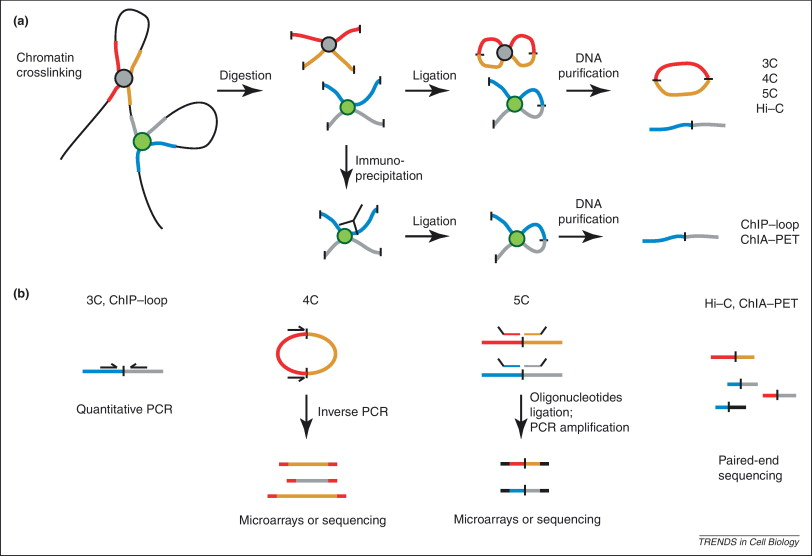
\includegraphics[width=\textwidth]{figures/biology/CompareChromosomeCapture}
  \medskip
  \small
  Chromatin is uniformly cross-linked and digested with a restriction enzyme.
  Bound sequences are immunoprecipitated or biotinylated, depending on the
  assay, and strands are ligated.  Ligation yields novel chimeric sequences
  which are purified.  The number of interactions are assess by qPCR in
  the canonical \gls{3C} method and ChIP-loop, inverse PCR in 4C, multiplexed
  sequencing with oligonucleotides in 5C, and paired end sequencing in Hi-C
  and ChIA-PET\@.  Adapted from Montavon et al. \citep{montavon2012}.
\end{figure}


The perceptive reader will note that much can go wrong in a \gls{3C} experiment. Every \gls{3C} method involves some level of digestion, ligation,
and amplification, and errors may be introduced at each step.  In particular, Dekker provides guidelines for three important control steps to
ensure the methodology remains integrous: control of PCR efficiency, determination of background random collisions and data
normalization \citep{dekker2006}.  Many derivative methods omit the PCR step, however all methodologies must be cognizant that
biases are introduced in any replacement protocol.

\section*{Topology and Fragility}

The first investigations into nuclear architecture were conducted by examining cell karyotypes.  Despite the development of the karyotype as a
tool for examining nuclear material in the early 20th century \citep{levitsky1924}, it wasn't until 1954 that the number of chromosomes in a human
cell were definitely described \citep{tjio1956}.  Early investigations into nuclear architecture, even using simple karyotypes, were
hampered by technical limitations and chromosomal phenomena such as \gls{non-disjunction} and breakage.  It is not surprising that soon after the
initial description the human chromosomal number, Debakan and colleagues characterized common sites where chromosomes would undergo breakage or
translocations.  They termed these regions \gls{CFS} \citep{leyden2008}.

Many particularities render studying fragile sites difficult.  The first difficulty is semantic; chromosomal fragile sites are not precisely
defined in the literature.  When a study is performed that encompasses fragile sites, typically one of three definitions is used: regions
that are particularly sensitive to forming gaps or breaks on metaphase chromosomes \citep{glover2005}, sites where chromatin fails to compact
under mitosis \citep{leyden2008}, and non-randomly distributed loci that exhibit an increased frequency of breakage under replicational
stress \citep{franchitto2013}.  For the purposes of this discussion, a \gls{fragile site} is a region on the chromosome prone to
forming complex rearrangements, particularly double-strand breaks, repeat extensions, and translocations, when subjected to replicational stress.
These rearrangements play a pivotal role in many severely deliberating genetic diseases.

Fragile sites come in two flavors: common fragile sites (CFS) and rare fragile sites (RFS).  Fragile sites are classified into a group based on their
prevalence in the population, and the conditions under which their fragility is induced \citep{leyden2008}.  Common fragile sites are thought to be common
to all humans, while rare fragile sites may be expressed in small fraction (less than 5\%) of the population \citep{wells2006}.

Rearrangements play pivotal roles in severely debilitating genetic diseases such as Fragile X Syndrome.  All males and an estimated that 60\% of females
with repeat anomalies near the FRM1 gene on the X chromosome suffer from severe mental handicap due to these alterations \citep{sutherland1995}. Additionally,
fragile sites are often found rearranged in human cancers \citep{glover2005}.  Despite these findings, the basis of fragility in fragile sites is still an
unanswered question.

\chapter{Methods}

\section{Data Collection}

The cell lines used in this thesis are the IMR90 lung fibroblast cell line and the H1 human embryonic stem
cell line.  Unless otherwise stated, the data obtained for these cell lines are wild type, reference sequences
and mappings.

\subsection{Processing Chromatin Interaction Data}

The Hi-C data sets used in this thesis were obtained from the Gene Expression Omnibus (GEO)\cite{edgar2002}
as Sequence Read Archive (SRA) files\footnote{Accession Number %
\href{http://www.ncbi.nlm.nih.gov/geo/query/acc.cgi?acc=GSE43070}{GSE43070}.}.  A bash script was written
to download six experimental replicates of IMR90 cells and two replicates of H1 hESCs from GEO onto a
local machine for analysis.  Using the Hi-C library prepared by Imakaev and colleagues\cite{imakaev2012},
the chimeric reads were realigned to the human genome (UCSC build hg19) using the Bowtie2 alignment
algorithm\cite{langmead2012} with default parameters.  The interactions matrices were prepared and processed
using custom scripts written in the Python programming language.

% FIXME Make sure appendix numbers/labels are correct
I noted that the aligned interactions matrices by replicate are highly correlated (Spearman's $\rho \gte 0.69$)  % FIXME p-value!
for both cell lines, and significantly different from random (Appendix III).  The

% TODO Do the python statistics here to validate that the data is good.  This includes:
% 1) Spearman's between H1 and IMR90
% 2) Spearman's between H1 replicates
% 3) Compute a "random" Hi-C map and take correlation between these
% 4) Show that normalization does not significantly decrease the correlation
% 5) Include p-values for everything I state


\subsection{DNA Methylation Analysis}

% TODO

\subsection{Gene Expression and Pathway Analysis}

Affymetrix gene expression microarray data for IMR90 and H1 hESCs were obtained from GEO (GSE2672\cite{kim2005}
and GSE54186\cite{kim2014}, respectively).  Probe annotations were downloaded from the Affymetrix site for
the Human Genome U133v2 array, and remapped to genes from UCSC\@.  Noticing that expression profiles for replicates
were similar, the gene expression levels for each cell line were calculated by averaging across replicates, and
taking the log2 transform of the averaged signal, yielding signal for $23,100$ genes.

% TODO Kolmogorov-Smirnov test w/ normal distribution

To understand expression changes during differentiation from stem cell to lung cell, I subtracted the lung expression
signal from the stem cell line.  Taking the log2 transform yields the fold change in gene expression level per gene.
Two groups of genes were selected for further analysis: the 100 most upregulated genes and the 100 most downregulated
genes.  I was curious to find out whether classes of genes were changing together.  Using the ConsensusPathDB
tool\cite{kamburov2012}, I performed over-representation analysis for pathways and gene ontologies.

\subsection{Histone Binding}

% TODO

\subsection{Chromatin Accessibility Assay}

% TODO

Additionally, analyzed tracks for DNA methylation at base pair
resolution were obtained from GEO\cite{lister2009}.  The liftOver tool from
the University of California Santa Cruise was used to update the methylation
data from human genome build hg18 to hg19 for meaningful comparison\cite{hinrichs2006}.
For detailed data collection notes, see Appendix I.

The detailed description of the treatment protocol used in creating the Hi-C
library can be found in the original paper\cite{ren2013}.  Briefly, the IMR90
cells were cultured in growth media.

The cell lines were prepared with no treatment according to the protocol
described by Dekker and colleagues\cite{dekker2013}.  In brief, the cells
are washed with a formaldehyde fixation solution to cross-links DNA and
protein molecules near each other in genomic space.  The cells are
lysed and the nuclear contents are treated with a non-specific restriction
enzyme, \textit{HindIII}.  After restriction, the remaining nuclear material
is washed so that the remaining contents are short DNA sequences or cross
-linked DNA-protein complexes.  The DNA reads are labeled with a biotin
marker and ligated at low concentrations that favor within ligation between
reads bound to the same complex.  The reads are captured and sequenced,
building what is known as a Hi-C library.

%% Regulatory Elements from Ensembl

%% Translocations from COSMIC

%% Genes from Biomart
%% Hg19 from UCSC


\section{Mapping and Alignment}

A Hi-C library is formed largely of \textit{chimeric} DNA sequences,
sequences composed of material from more than one source.  The ligation process
creates novel DNA sequences with a portion of sequence from one region of
the genome and the remaining portion from a different genomic region.  In
order to discover to which two regions each probe corresponds, the probes
must be realigned to the human genome.  Previous methods (\textit{citation needed})
have truncated reads to a fixed cutoff size before realignment with a short
read alignment algorithm.  In a recent paper, Imakaev and colleagues
describe an algorithm to repeated align reads with different truncation sizes
and analyzing reads with the maximum alignment score\cite{imakaev2012}.  We followed
this procedure to realign the IMR90 Hi-C libraries for six replicates to
the human genome build 19 (CRCh38/hg19), with an average of XX million reads
mapped per replicate.

\section{Normalization of Contact Maps}

Understanding and accounting the biases inherent in a data set is vital to
producing accurate, biologically relevant analysis.  To this end, several methods
have been proposed identify biases and normalize contact maps between replicates
and experiments\cite{yaffe2011}\cite{hu2012}\cite{yang2014}.  The earliest methods on low
resolution samples did not perform any normalization at all\cite{aiden2009};
however, as higher resolution data sets have come available, better
normalization methods are being explored to identify reproducible,
fine-grained chromatin structures.

Normalizing data from Hi-C experiments is quite challenging.  As previously
discussed, the Hi-C data sets are heterogeneous in nature, incorporating
interactions from cells in every position of cell cycle.  As evidence of phenomena,
the interaction matrices produced by the Hi-C experiments have nonzero contact
probabilities between nearly every genomic coordinate\cite{dekker2013}.  This
finding is further reinforced by the observation that single cell Hi-C analysis
shows high variability in chromatin architecture\cite{nagano2013}.  Despite this
variability, existing normalization techniques for Hi-C data sets typically
assume the majority of the cells in the sampled ensemble are in a static
chromatin conformation reflective of \textit{in vivo} cell populations.

One approach to normalization described by Yaffe and colleagues\cite{yaffe2011}
attempts to describe the total interaction frequency between loci as the product
of a true interaction frequency and a set of experimental biases.  These biases
are present in all chromosomal capture techniques.  They include biases due to
PCR in efficiency, read depth per region, sequencing bias, chromatin compaction,
and random background collisions during ligation\cite{benner2014}\cite{dekker2006}.


% results.tex

\chapter{Results \& Discussion}

\section*{The number of interactions is a function of distance and chromosome}
In earlier treatments of the Hi-C data sets, the analysis of folding patterns by various groups\cite{imakaev2012}\cite{dixon2012}
the density of bound probes as a function of distance for the entire genome.  However, in our analysis, we remark that chromosomes
have heterogeneous scaling properties, as seen figure~\ref{fig:interactionScaling}.

\begin{figure}[h]
  \caption{Number of interactions as a function of distance.}\label{fig:interactionScaling}
\end{figure}

We find that the relative ordering of these curves are reproducible between replicates (Pearson=?).  This implies th.

Notably, the scaling ratios are unchanged by normalization, indicating that scaling may be a property of the underlying distribution
rather than an artifact of out data processing.  Indeed, this indicates that perhaps normalization should be performed, as is
done in HiCNorm\cite{hu2012} on a chromosome by chromosome basis, estimating different background distributions for each chromosome
rather than using a generalized fitting algorithm such as IPF\@.  This.

\section*{Differentiation induces fibroblast-specific gene products in IMR90}

The transition from embryonic pluripotency to a specialized cell type naturally introduces a change in the expressed cell products.
Using Affymetrix microarrays, we observe that the overall trend towards differentiation marginally increases gene expression across
the entire proteome (mean=?).  This observation is not surprising, and is thoroughly documented in the literature\cite{tuomela2012}
for various cell types.

We then sought to understand how expression changes were related to molecular function in the cell.  Using the ConsensusPathDB
tool\cite{kamburov2012}, we performed both over expression and gene ontology analysis of the 1\%  largest positively and negatively
and signalling pathways.  Furthermore, downregulated genes are involved in transcriptional regulation of pluripotent stem cells.

We asked whether transcriptional upregulation during differentiation could predict mutations, lesions, or break points seen in lung
cancer studies.  We acquired data for every type of lung cancer lesions from the Catalogue of Somatic Mutations in Cancer
(COSMIC)\cite{forbes2009} by gene.  Interestingly, the frequency of lesions reported by COSMIC was uncorrelated to those genes
expression changes (Pearsons $0.07$, $p < 1 \times 10^{-18}$).  There are a number of potential causes for the lack of signal in
our expression data.  Perhaps the expression arrays are not able to identify gene fusion products, a non-negligible portion of
the COSMIC mutation database.  More likely, as reported recently by Ashworth and colleagues, it is mutations in transcription factors
that cause gene expression changes in cancers, rather than in the genes themselves\cite{ashworth2014}.

\section*{Contact maps of cell lines change drastically during differentiation}
% TODO

\section*{Cancerous lesions are in close proximity to topological domains}

% discussion.tex
\chapter{Discussion}

The shadowy mechanisms that bring about catastrophic diseases such as cancer are slowly being elucidated.  Using previously published normalization
algorithms, we were able to reproduce topological domain and chromatin compartments seen in previous papers \citep{dekker2012, dixon2012}. Our results
yielded two intriguing findings: chromatin compartments do not seem to serve a regulatory role, and cancerous lesions are clustered within domains
and domain boundaries.

\section*{Chromatin Compartments and Regulation}

The original Hi-C experiment revealed that the genome can be compartmentalized by \gls{PC} into two characteristic classes, arbitrarily
labeled A and B.  Lieberman-Aiden and colleagues showed positive correlations between compartment identity, gene density, and chromatin
accessibility, concluding that compartment A consists of largely open chromatin, while compartment B is densely packed \citep{aiden2009}.
Interestingly, we did not observe any correlation between the eigenvector and gene expression data (via genome-wide mRNA expression,
Spearman's $\rho = -0.014$, $p-$value negligible; Figure~\ref{fig:expressionChangeByCompartment}).  Furthermore, shifts in compartment character did not correlate to
changes in gene expression level (Spearman's $\rho = -0.01$, $p-$value negligible).  Given these results, it seems unlikely that cells regulate
gene expression at the compartment level.

\section*{Lesions and Topological Domains}

The pursuit of an underlying topological explanation for genomic fragility is not yet over.  We demonstrated that boundary regions of topological
domains show higher numbers of mutations than expected on average, yet the mechanistic insight into the causes of these mutations is yet to be
fully described.  Early results show differentiable peaks for certain \gls{DNA} binding proteins; however, a full set of epigenetic factors (histone
modifications, transcription factors, etc) should be analyzed for a cohesive understanding of their importance.  The origin of genomic fragility on
the macroscopic level defined by common fragile sites is yet undiscovered, and we did not observe a relationship between the macro-molecular
compartments seen by \citet{dekker2012} and fragile site placement.  It may be that fragile sites are organized on higher orders, such as chromosome
territories.

Many questions remain: what types of lesions occur most frequently at domain boundaries?  How are the genome's fractally structured topological
domains regulated?  In this analysis, we studied lung cancer specific mutations; however, there is strong evidence that boundaries are conserved
across cell types \citep{dixon2012,pope2014}.  Future studies can expand off this base, searching for mutations across many different cancers to
identify a conserved mechanism.  Finally, there is still much work to be done in characterizing the role that topological domains play in the
greater scheme of genome architecture and expression.  Only once we understand the intricate interactions surrounding these domains, will we be
equipped conquer the diseases that plague them.


%
% APPENDIX
%
\appendix%
\appendixpage%
\addappheadtotoc%

% appendix.tex
\chapter{Data Collection}

Methylation data was downloaded from the Salk Institute for Biology Studies in
two files from two biological replicates.  Each file contained $\sim600$ million
reads from the

\begin{table}
  \centering
  \begin{tabular}{lccr}
    \hline
    Replicate & Hg18 Reads & Hg19 Reads & Unlifted Reads \\ \hline
    1 & 563,354,527 & 563,071,323 & 566,408 \\
    2 & 620,520,572 & 620,227,842 & 585,460 \\
    \hline
  \end{tabular}
  \caption{Genomic methylation data for IMR90}
\end{table}

\chapter{Data Migration to Human Genome Build 19}

To make valid comparisons between disparate data sets, it is crucial to ensure all data sets are aligned to the same
build of the human genome.  A genome build is a haploid assembly of sequences from several individuals published by
the NCBI to provide a reference for an organism gene and feature set, though not necessarily every allele.  A build assembly
refers to a particular published sequence annotation set.  Human Genome Build 19 (HG19) is the University of California Santa
Cruz nomenclature for the NCBI Build GRCh37 published in 2009\cite{lander2001}.

In this thesis, the methylation and histone assays were all reported against human genome build 18.  Experiments aligned
against previous builds of the human genome may be updated informatically, either by re-alignment of the
sequence probes or through coordinate transposition.  The UCSC Genome Browser provides a command line utility liftOver for
batch coordinate conversion.  Each file was unzipped and updated to HG19 prior to further analysis using the liftOver tool.

\begin{table}
  \centering
  \begin{tabular}{lccr}
    \hline
    Sample & HG18 Reads & HG19 Reads & Unlifted Reads \\ \hline
    H3K27ac & 16374518 & 16371125 & 3,393 \\
    p65 & 16371125 & 6165230 & 947 \\
    H3K4me1 & 18713234 & 18709033 & 4201 \\
    H3K36me3 & 15808706 & 15807726 & 980 \\
    CTCF & 5501307 & 5499946 & 1361 \\
    \hline
  \end{tabular}
  \caption{Genomic methylation data for IMR90}
\end{table}

\chapter{Iterative Alignment of Probes}

Probes were aligned to the human genome build hg19 using procedures outlined by
Imakaev and colleagues\cite{imakaev2012}.  The chimeric nature of the reads
requires that probes be aligned iteratively, starting from a small, truncated
region from the beginning of the read, mapping this truncated area, increasing
the truncation size and recursing a fixed number of steps or until the alignment
scores become sufficiently poor.  Due to the large number of reads requiring
alignment, we opted to use a fixed truncation length (based on sequence length)
and four steps in the iterative alignment protocol.  The calculation
for the truncation and step size can be found in the the iterativeMapping.py
script provided in the Appendix: Code.  Most reads were 100 base pairs, resulting
in an initial truncation length of 28 base pairs, and step size of 18 base pairs.

Using the mapping functionality from the hiclib python package\cite{imakaev2012},
sequences from the six experimental replicates were realigned to the genome.  The
alignment employed the fast Bowtie2 alignment algorithm\cite{langmead2012}.  Once
aligned, the probes were stored as an interaction matrix in the high performance
HDF5\cite{hdf5} data format, a total of 25Gb for all replicates.

Statistics for iterative alignment are given below:

\begin{center}
  \begin{table}
    \begin{tabular}{l l}
    Total Reads & 2,124,453,478 \\
    Total DS Reads & 1,422,870,270 \\
    Valid Pairs & 713,897,554 \\
    Filtered Reads & 457,298,174 \\
    Percent \textit{trans} Reads & 49.42\% \\
    \end{tabular}
  \end{table}
\end{center}


\chapter{Data Validation}

In order to make meaningful comparisons between data sets (replicates,
in this case), we must show that some degree of relationship exists between
the data sets and comparisons or combinations of the data from disparate sets
are valid to a degree of uncertainty.  It is also essential to understand if the
experimental replicates indeed managed to replicate the conditions of the primary
experiment, or if experimental errors prevent the comparison between replicates.

Spearman's Rank Correlation Coefficient (denoted by the Greek letter $\rho$) is
a non-parametric measure of association between two variables.
Spearman's coefficient assumes some monotonic relationship between variables,
rather than a linear relationship (as in Pearson's), making it appropriate
to compare the IMR90 interaction data sets.  The formula for Spearman's $\rho$ is
given as follows:

\begin{equation}
\rho = 1 - \frac{\sum_{i=1}{n}(d_i^2)}{n(n^2 - 1)}
\end{equation}

where $\rho$ is the correlation coefficient taking values between $-1$ and $+1$,
$d_i = x_i - y_i$ where $x_i, y_i$ are ranks derived from the raw scores $X$ and
$Y$ respectively.

The first replicate IMR90 interaction data set was labeled the primary data set
and the remaining five were compared using Spearman's Rank Correlation.  The
results are given in Table X.

\begin{table}
  \begin{tabular}{|c|*{6}{c|}}
    \toprule
    \textbf{R1} & 0.83 & 0.77 & 0.77 & 0.75 & 0.71 \\ \midrule
    0.83 & \textbf{R2} & 0.82 & 0.83 & 0.79 & 0.75 \\ \midrule
    0.77 & 0.82 & \textbf{R3} & 0.77 & 0.74 & 0.73 \\ \midrule
    0.77 & 0.83 & 0.77 & \textbf{R4} & 0.75 & 0.71 \\ \midrule
    0.75 & 0.79 & 0.74 & 0.74 & \textbf{R5} & 0.69 \\ \midrule
    0.71 & 0.75 & 0.73 & 0.71 & 0.69 & \textbf{R6} \\ \midrule
  \end{tabular}
  \caption{Spearman's $\rho$ across all data sets.}
\label{tab:correlations}
\end{table}


\chapter*{Supplementary Information}

\newpage
\section*{Public data sets}

\begin{table}[H]
  \begin{threeparttable}
    \caption{Public data sets analyzed}
    \begin{tabularx}{\textwidth}{@{}p{4cm}lp{7cm}@{}}
      \toprule
      Data set & Accession & Reference \\
      \midrule % column names
      Lung Fibroblast Hi-C, \gls{hESC} Hi-C & GSE43070 & \bibentry{jin2013} \\
      TCGA Lung Cancer Mutations            & {}       & \bibentry{cerami2012} \\
      H1 \gls{hESC} Gene Signatures          & GSE54186 & \bibentry{kim2014} \\
      IMR90 Gene Signatures                 & GSE2672  & \bibentry{kim2005} \\
      \bottomrule
    \end{tabularx}
    \begin{tablenotes}
      \item All data sets were obtained as of December 2014.
    \end{tablenotes}
  \end{threeparttable}
\end{table}

\newpage
\section*{Interaction Heatmaps}

\begin{figure}[H]
  \caption{Whole Genome Heatmaps}\label{fig:WholeGenomeHeatmaps}
  \begin{minipage}{0.5\textwidth}%
    \includegraphics[width=\textwidth]{./figures/supplementary/hm/hesc_raw_1Mb.png}
  \end{minipage}%
  \hfill
  \begin{minipage}{0.5\textwidth}
    \includegraphics[width=\textwidth]{./figures/supplementary/hm/hesc_ic_1Mb.png}
  \end{minipage}
\end{figure}

\begin{figure}[H]
  \begin{minipage}{0.5\textwidth}%
    \includegraphics[width=\textwidth]{./figures/supplementary/hm/imr90_raw_1Mb.png}
  \end{minipage}%
  \hfill
  \begin{minipage}{0.5\textwidth}
    \includegraphics[width=\textwidth]{./figures/supplementary/hm/imr90_ic_1Mb.png}
  \end{minipage}
  \medskip
  \small
  Genome heatmaps constructed from raw (left) and normalized (right) interaction maps.
  Chromosomes are arranged as blocks on the diagonal.  Each light colored block on the
  diagonal shows regions of increased interactions.  White bands correspond to regions
  of noise removed due to noise, typically around centromeres and telomeres.
\end{figure}

\begin{figure}[H]
  \caption{IMR90 Chromosome 2 Banding}\label{fig:Chrom2Banding}
  \begin{minipage}{0.5\textwidth}%
    \includegraphics[width=\textwidth]{./figures/supplementary/hm/IMR90-R1-200k-Chr2.png}
  \end{minipage}%
  \hfill
  \begin{minipage}{0.5\textwidth}
    \includegraphics[width=\textwidth]{./figures/supplementary/hm/IMR90-R1-200k-Chr2.png}
  \end{minipage}
  \medskip
  \small
  IMR90 Replicates I and II\@.  The red and blue coloring reveals the banding patterns described by
  \citet{dekker2012}, indicating areas of above average or lower than average interactions.  These chromatin
  compartments are captured in the first two principal components.
\end{figure}


\begin{table}[H]
  \centering
  \caption{Mapping Statistics}\label{tab:hmstats}
  \begin{tabular}{cccc}
    \toprule
    Map & Total Reads & Post-Filtering & Percent \textit{Trans} \\
    \midrule
    hESC R1  & 199955400 & 18295668  & 48.6\% \\
    hESC R2  & 433584106 & 125581108 & 23.6\% \\
    IMR90 R1 & 349117513 & 90481608  & 37.3\% \\
    IMR90 R2 & 398642708 & 157378922 & 50.6\% \\
    IMR90 R3 & 528662422 & 72996792  & 59.9\% \\
    IMR90 R4 & 463140318 & 53109981  & 54.2\% \\
    IMR90 R5 & 203181628 & 41901503  & 46.9\% \\
    IMR90 R6 & 181708889 & 41429368  & 49.0\% \\
    \midrule
    Total & 2757992984 & 601174950 & {} \\
    \bottomrule
  \end{tabular}
\end{table}

\section*{Principal Components}

We calculated Spearman's correlation coefficients between principle components for each data set.

% data from  pca/correlations/*.csv
\begin{table}[h]
  \centering
  \caption{Correlation of PC1 between all experimental replicates}\label{table:PC1Correlations}
  \begin{tabularx}{\textwidth}{@{}cccccccc@{}}
    \toprule
    \multicolumn{6}{l}{IMR90} & \multicolumn{2}{l}{hESC} \\
    \midrule
    \textbf{R1} & 0.981       & 0.972       & 0.983       & 0.983       & 0.977       & 0.656       & 0.658 \\
    0.981       & \textbf{R2} & 0.985       & 0.982       & 0.976       & 0.974       & 0.654       & 0.652 \\
    0.972       & 0.985       & \textbf{R3} & 0.982       & 0.977       & 0.980       & 0.634       & 0.629 \\
    0.983       & 0.982       & 0.982       & \textbf{R4} & 0.986       & 0.982       & 0.655       & 0.655 \\
    0.983       & 0.976       & 0.977       & 0.986       & \textbf{R5} & 0.98        & 0.633       & 0.633 \\
    0.977       & 0.974       & 0.980       & 0.982       & 0.985       & \textbf{R6} & 0.610       & 0.607 \\
    0.656       & 0.654       & 0.634       & 0.655       & 0.633       & 0.610       & \textbf{R1} & 0.973  \\
    0.658       & 0.652       & 0.629       & 0.655       & 0.633       & 0.607       & 0.973       & \textbf{R2}    \\
    \bottomrule
  \end{tabularx}
\end{table}

We also examined the scree plots of each \gls{PC} by experiment and replicate.  The plot for hESC R1 is included for reference.

\begin{figure}
  \centering

  \begin{subfigure}[b]{0.45\textwidth}
    \centering
    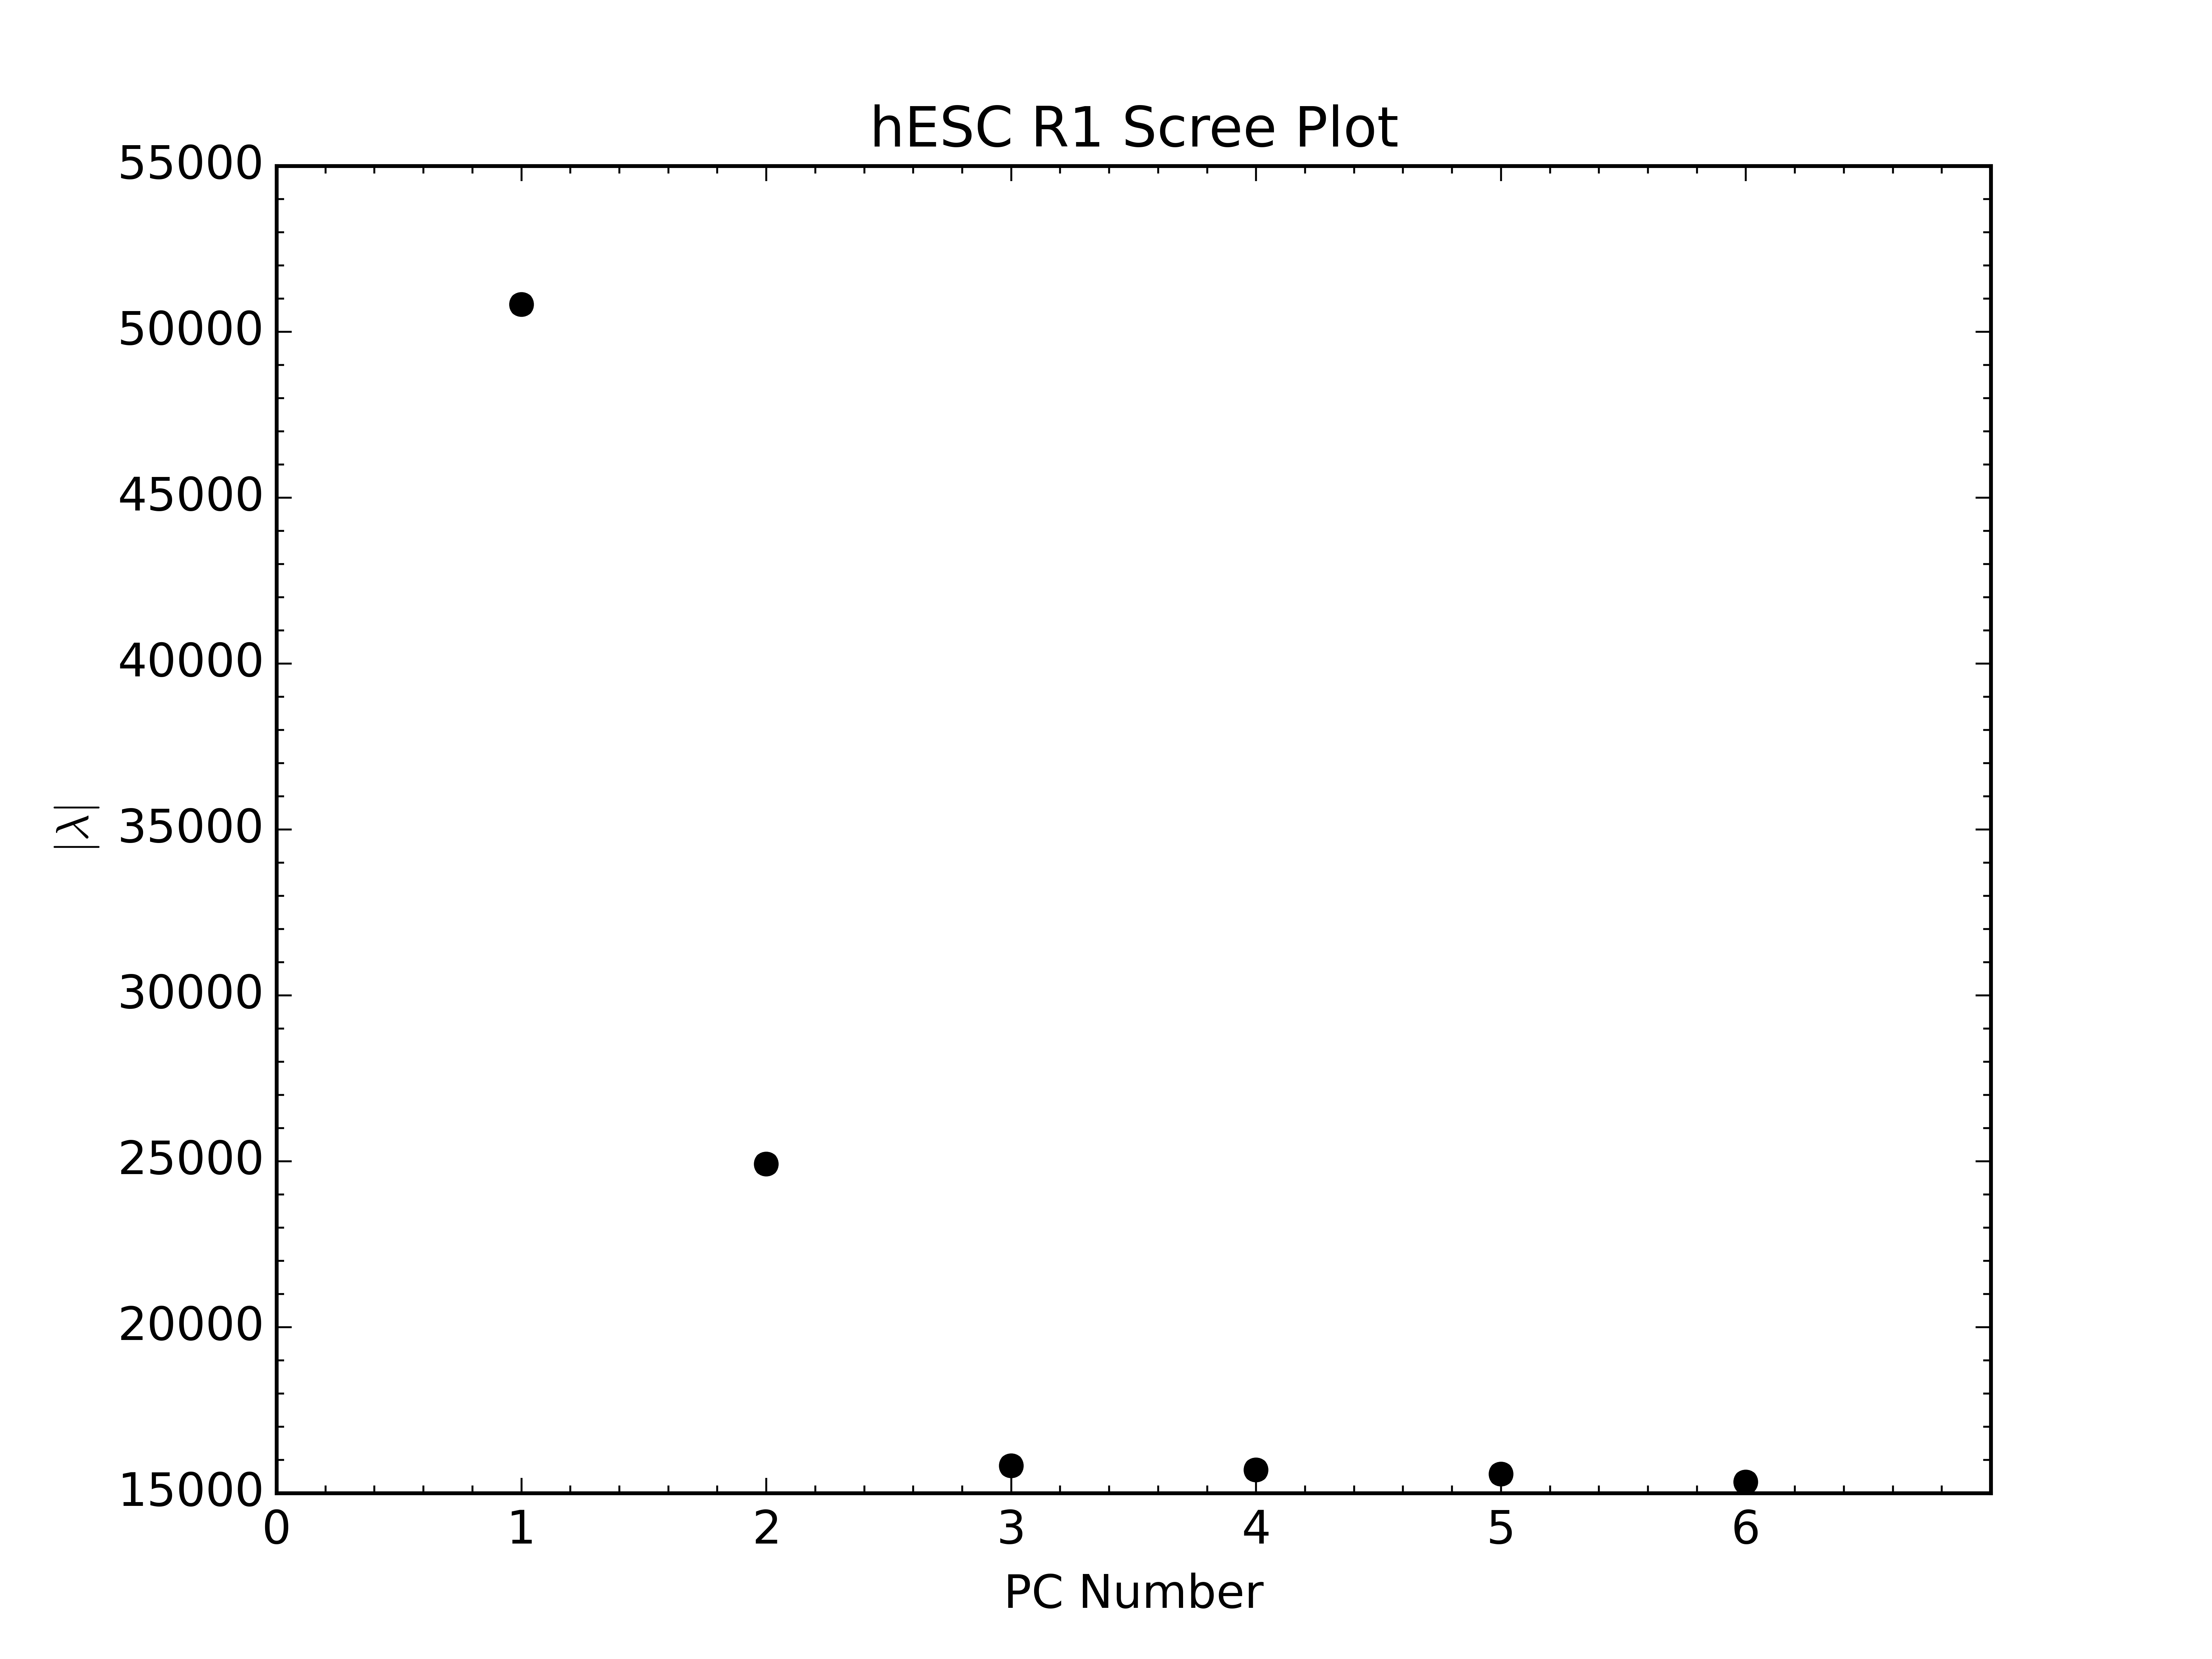
\includegraphics[width=\textwidth]{./fig/supplementary/hESC-R1-scree.png}\label{fig:hESCScree}
  \end{subfigure}

\end{figure}

\section*{Gene Expression Histograms}

\begin{figure}
  \centering
  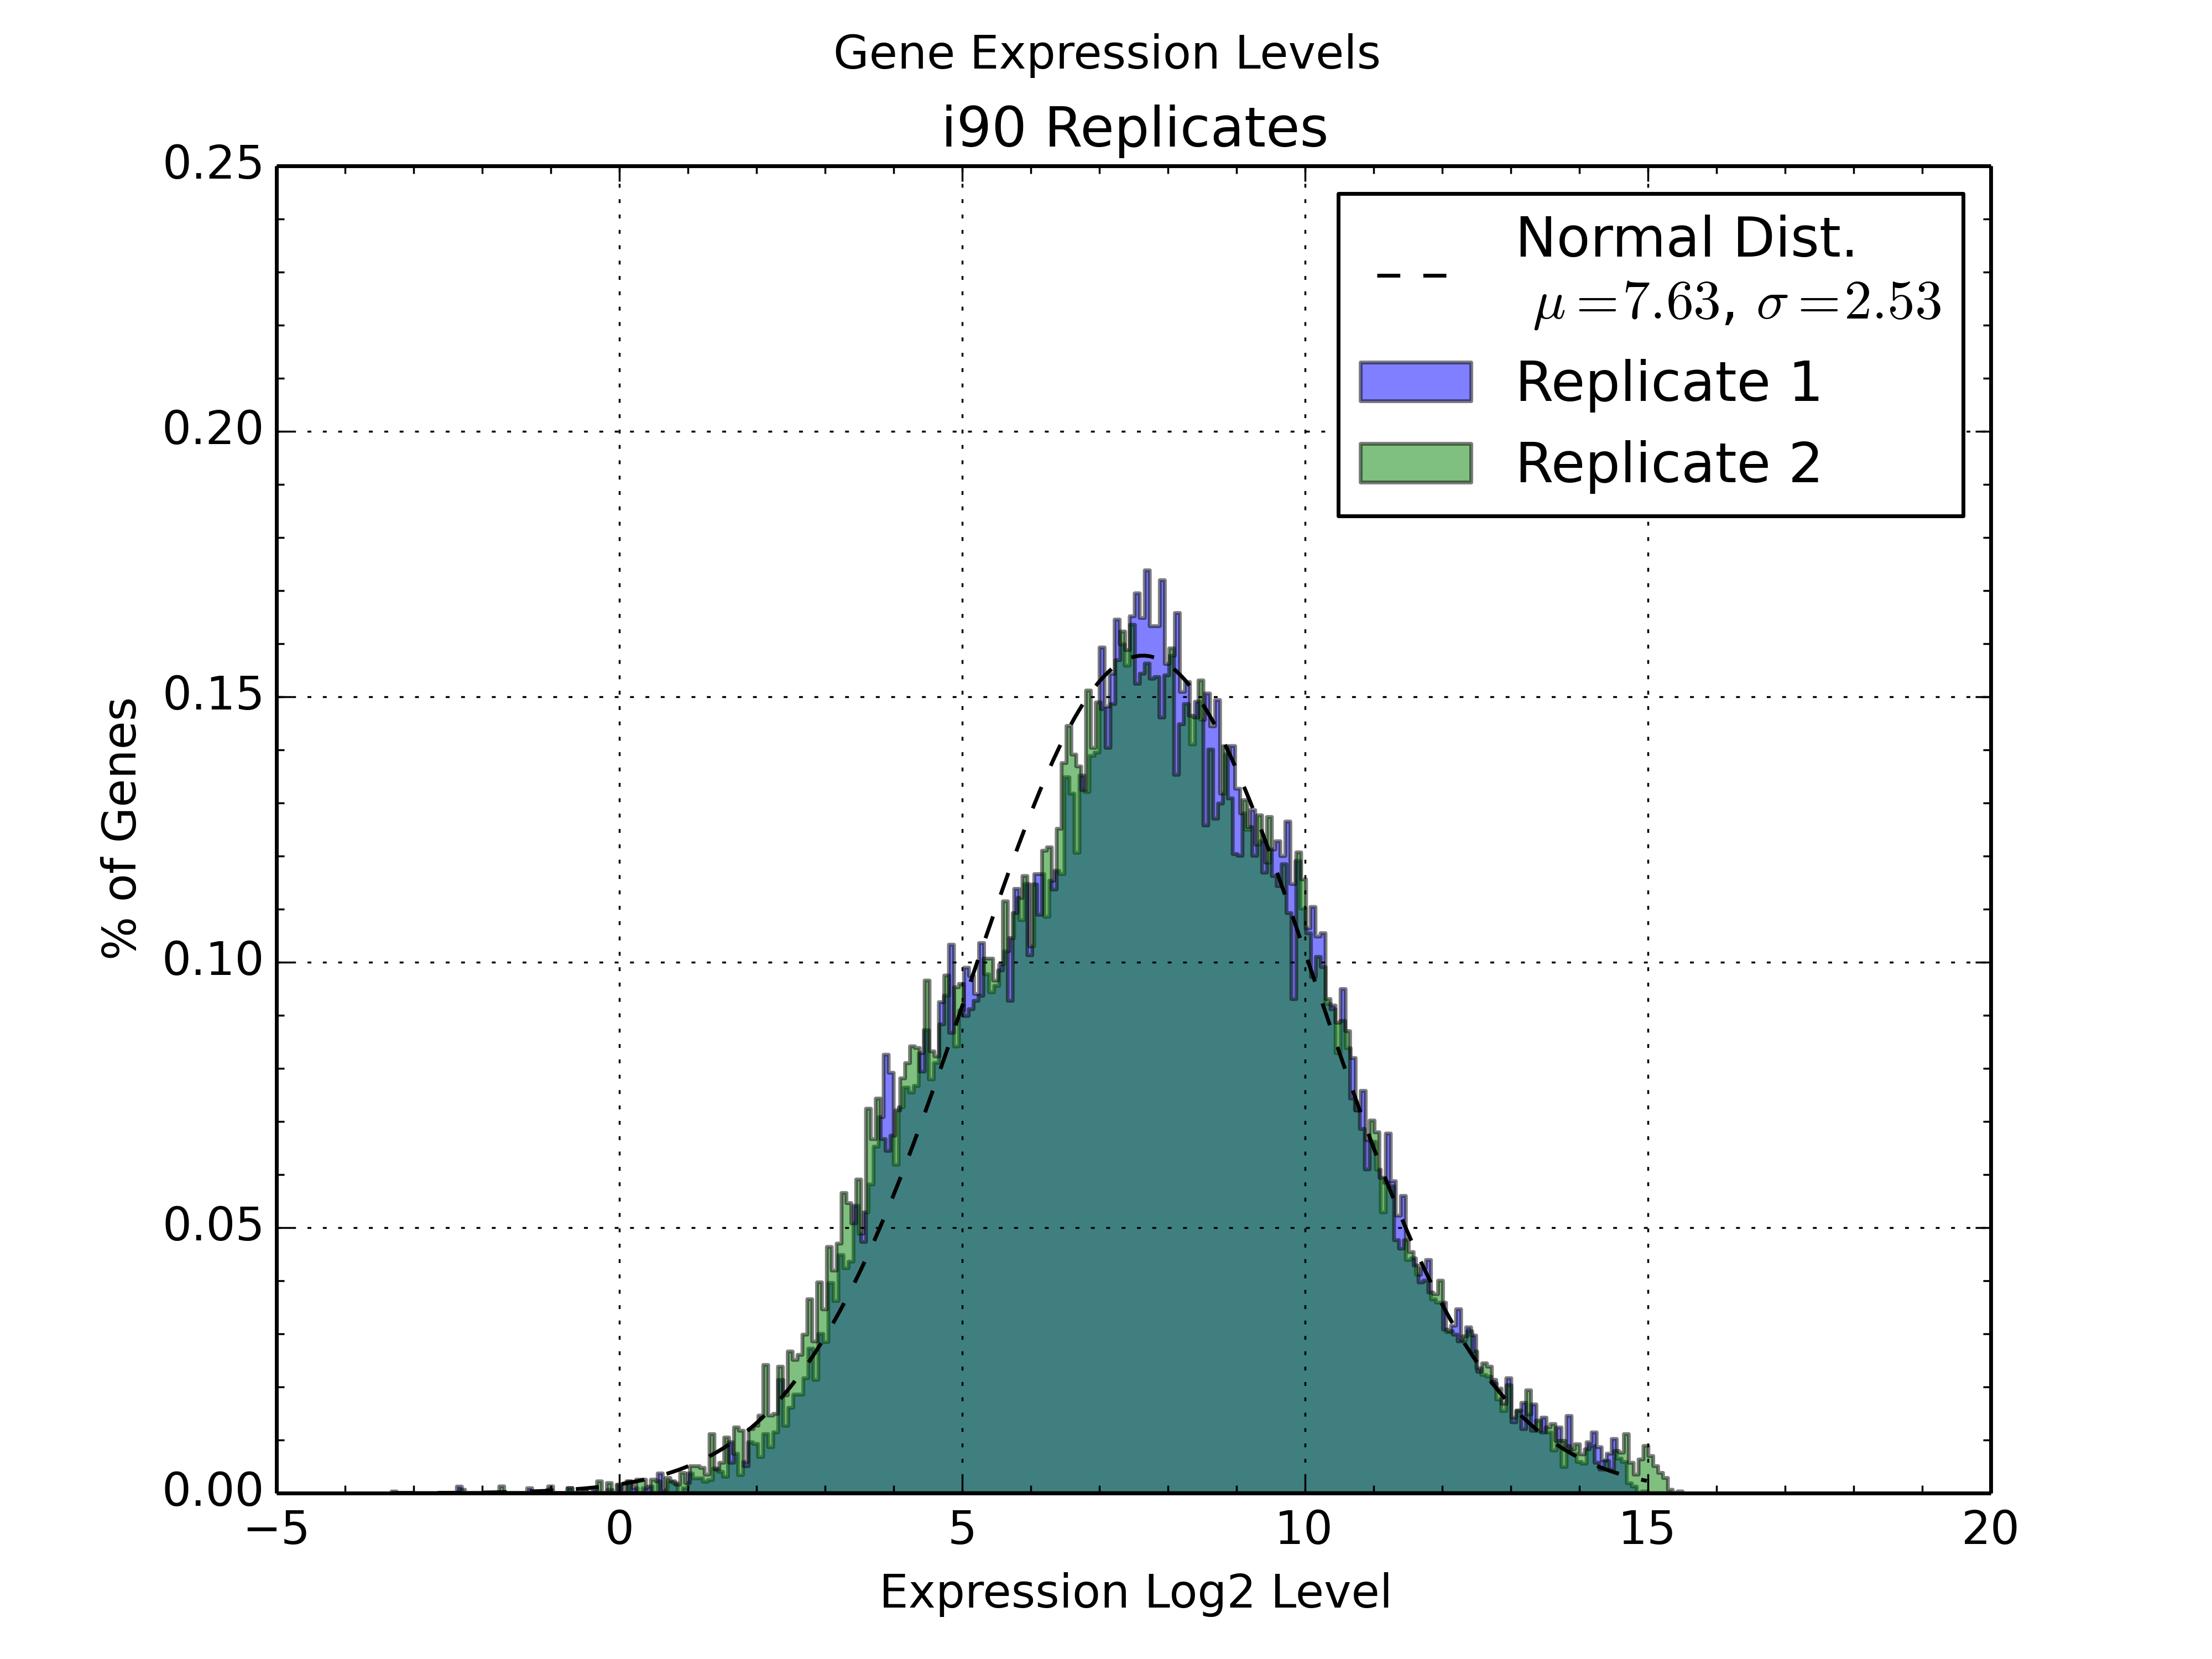
\includegraphics[width=\textwidth]{./figures/supplementary/i90-expression-levels.png}\label{fig:190Expression}
  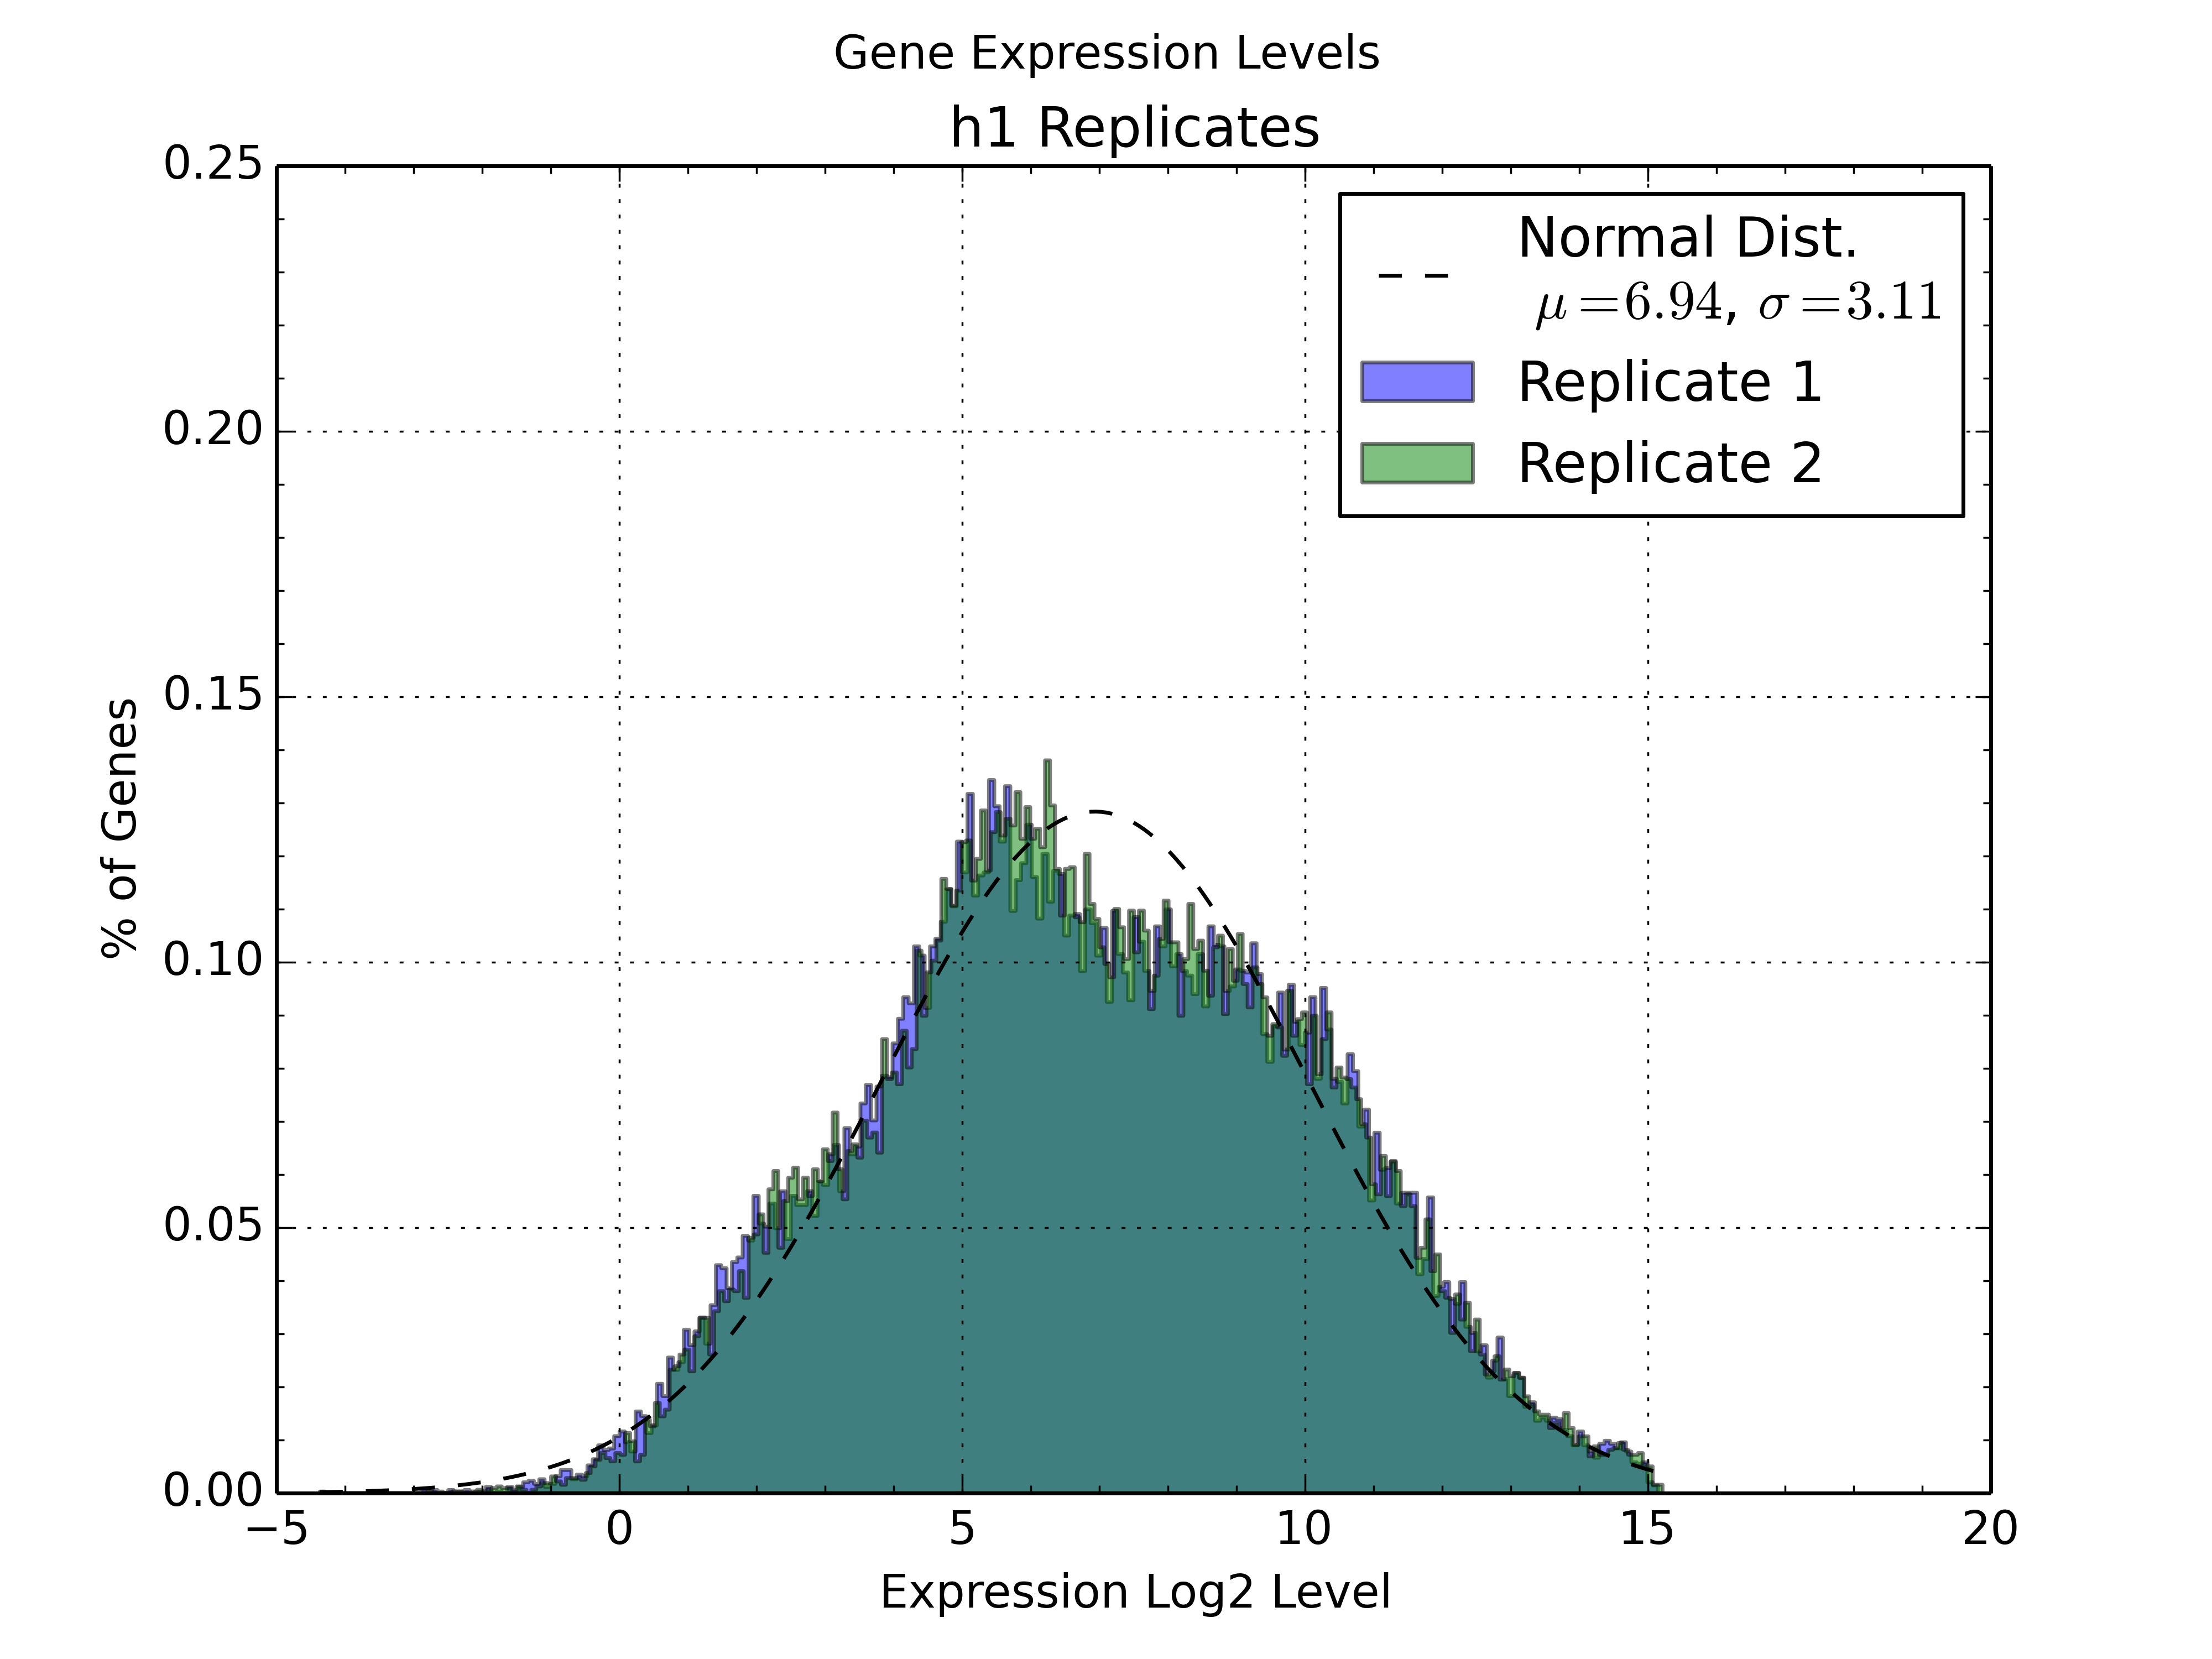
\includegraphics[width=\textwidth]{./figures/supplementary/h1-expression-levels.png}\label{fig:h1expression}
  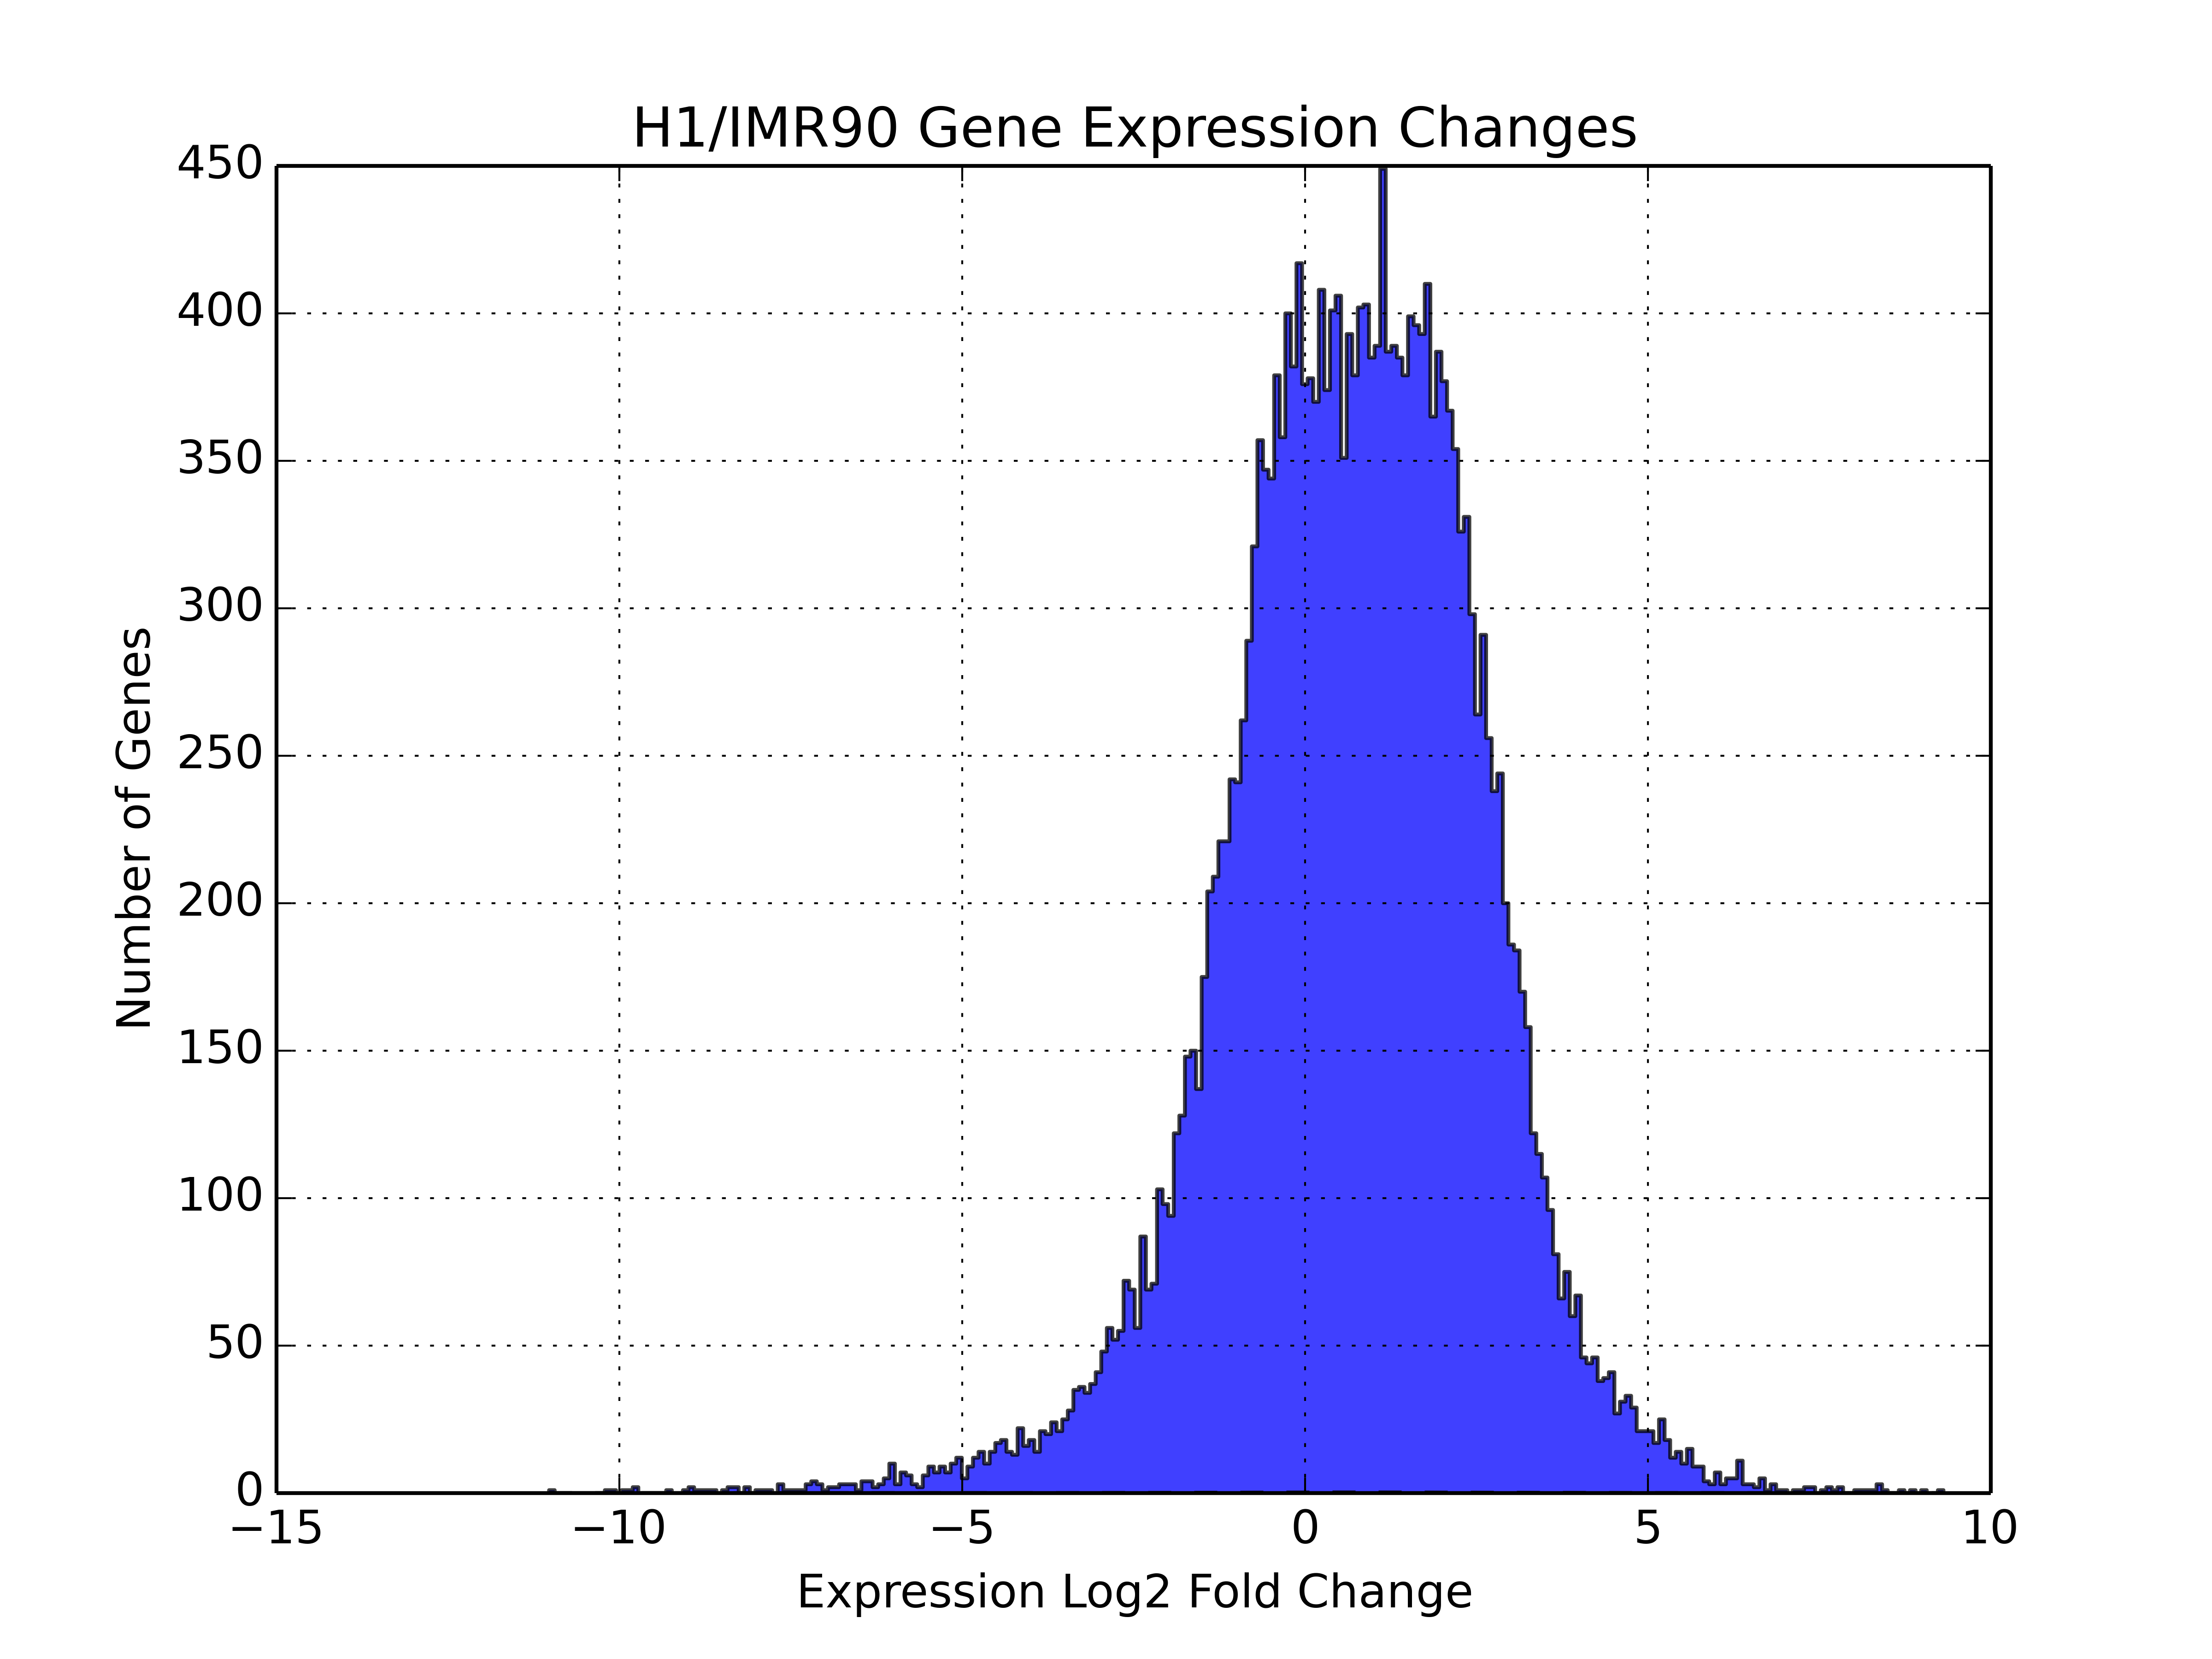
\includegraphics[width=\textwidth]{./figures/supplementary/expressionDelta.png}\label{fig:i90h1expression}
  \caption{Look at all these figures!}
\end{figure}


\newpage
\section*{Directionality Indices}\label{sec:SuppDirectionality}

Spearman's correlations calculated between directionality indices for different window sizes.  We calculated the
correlations for each window size.  The correlations for 100kb and 1Mb represented below show the spread of the
correlation coefficient values.

\begin{table}[H]
  \caption{Directionality Index Correlations}
  \parbox{.45\linewidth}{%
    \centering
    \tiny
    \caption{100kb Windows}\label{tab:SuppDi100kbWindows}
    \begin{tabular}{*{8}{c}}
      \toprule
      \multicolumn{6}{c}{IMR90} & \multicolumn{2}{c}{hESC} \\
      R1 & R2 & R3 & R4 & R5 & R6 & R1 & R2 \\
      \midrule
      1.00 & 0.84 & 0.80 & 0.83 & 0.80 & 0.78 & 0.78 & 0.77 \\
      0.84 & 1.00 & 0.91 & 0.92 & 0.82 & 0.86 & 0.86 & 0.79 \\
      0.80 & 0.91 & 1.00 & 0.91 & 0.80 & 0.83 & 0.83 & 0.77 \\
      0.83 & 0.92 & 0.91 & 1.00 & 0.84 & 0.86 & 0.85 & 0.81 \\
      0.80 & 0.82 & 0.80 & 0.84 & 1.00 & 0.80 & 0.79 & 0.82 \\
      0.78 & 0.86 & 0.83 & 0.86 & 0.80 & 1.00 & 0.82 & 0.77 \\
      0.78 & 0.86 & 0.83 & 0.85 & 0.79 & 0.82 & 1.00 & 0.77 \\
      0.77 & 0.79 & 0.77 & 0.81 & 0.82 & 0.77 & 0.77 & 1.00 \\
      \bottomrule
    \end{tabular}
  }%
  \hfill
  \parbox{.45\linewidth}{%
    \centering
    \tiny
    \caption{1Mb Windows}\label{tab:SuppDi1MBWindows}
    \begin{tabular}{*{8}{c}}
      \toprule
      \multicolumn{6}{c}{IMR90} & \multicolumn{2}{c}{hESC} \\
      R1 & R2 & R3 & R4 & R5 & R6 & R1 & R2 \\
      \midrule
      1.00 & 0.89 & 0.74 & 0.81 & 0.83 & 0.83 & 0.83 & 0.82 \\
      0.89 & 1.00 & 0.76 & 0.78 & 0.70 & 0.79 & 0.81 & 0.70 \\
      0.74 & 0.76 & 1.00 & 0.95 & 0.82 & 0.92 & 0.93 & 0.84 \\
      0.81 & 0.78 & 0.95 & 1.00 & 0.91 & 0.96 & 0.97 & 0.91 \\
      0.83 & 0.70 & 0.82 & 0.91 & 1.00 & 0.91 & 0.90 & 0.97 \\
      0.83 & 0.79 & 0.92 & 0.96 & 0.91 & 1.00 & 0.96 & 0.92 \\
      0.83 & 0.81 & 0.93 & 0.96 & 0.90 & 0.96 & 1.00 & 0.91 \\
      0.82 & 0.70 & 0.84 & 0.91 & 0.97 & 0.92 & 0.91 & 1.00 \\
      \bottomrule
    \end{tabular}
  }
\end{table}

\begin{figure}[H]
  \centering
  \caption{hESC Directionality Indices}\label{fig:hescDirectionalityIndices}
  
\includegraphics[width=\textwidth]{./figures/supplementary/directions/hESC-R1-1000kb.png}
  \vfill
  
\includegraphics[width=\textwidth]{./figures/supplementary/directions/hESC-R2-1000kb.png}
  \vfill
  
\includegraphics[width=\textwidth]{./figures/supplementary/directions/IMR90-R4-1000kb.png}
  \vfill
  
\includegraphics[width=\textwidth]{./figures/supplementary/directions/IMR90-R6-1000kb.png}
\end{figure}


\newpage
\section*{Domain Discovery}

Using the directionality indices computed on at 10kb resolution map, we computed domains by selecting the regions with the top
$10\%$ directionality bias.  Domains were further refined by intersecting between replicates and discarding non-overlapping
domains, leaving a small, conserved subset.  Overlaps between window sizes and replicates are shown in the figures below.

\subsection*{Domain Conservation}

\begin{figure}[thb]
  \centering
  \caption{Conserved Domains between IMR90 Replicates}
  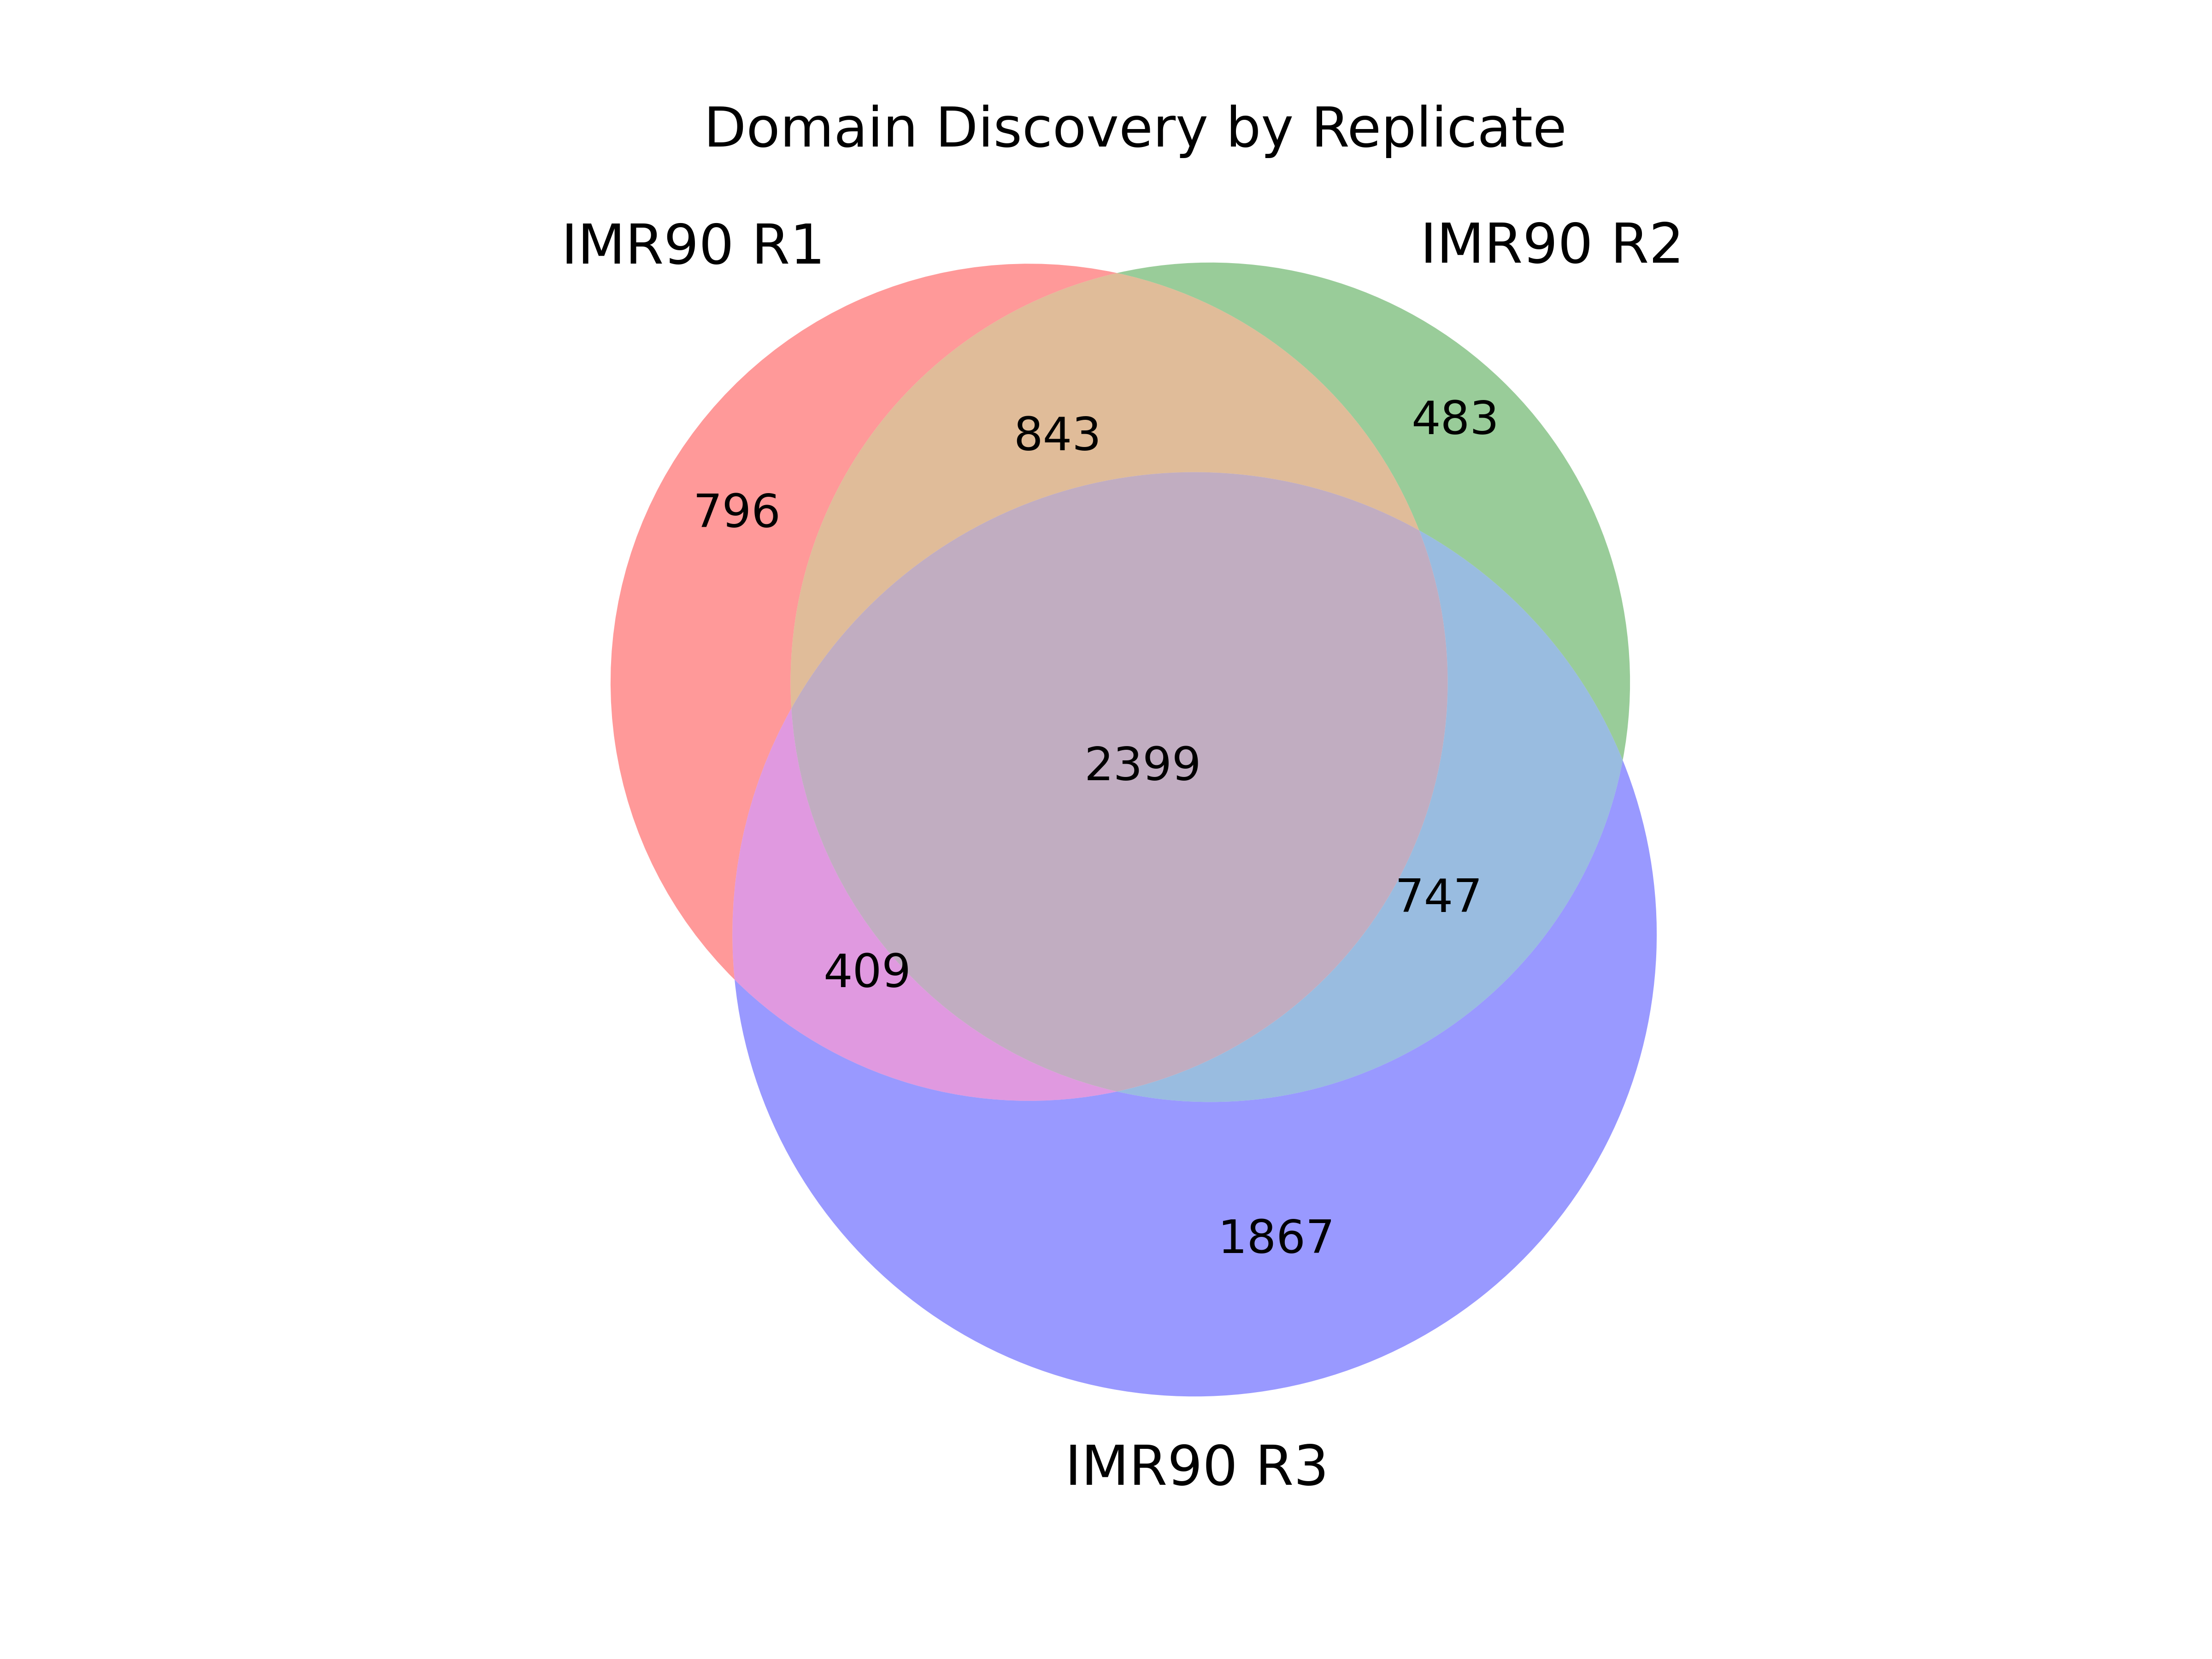
\includegraphics[width=\textwidth]{figures/supplementary/domains/venn3.png}\label{fig:SuppVenn3}
\end{figure}

\begin{figure}[thp]
  \caption{Domain Overlaps by Window Size}
  \begin{minipage}{0.45\textwidth}%
    \centering
    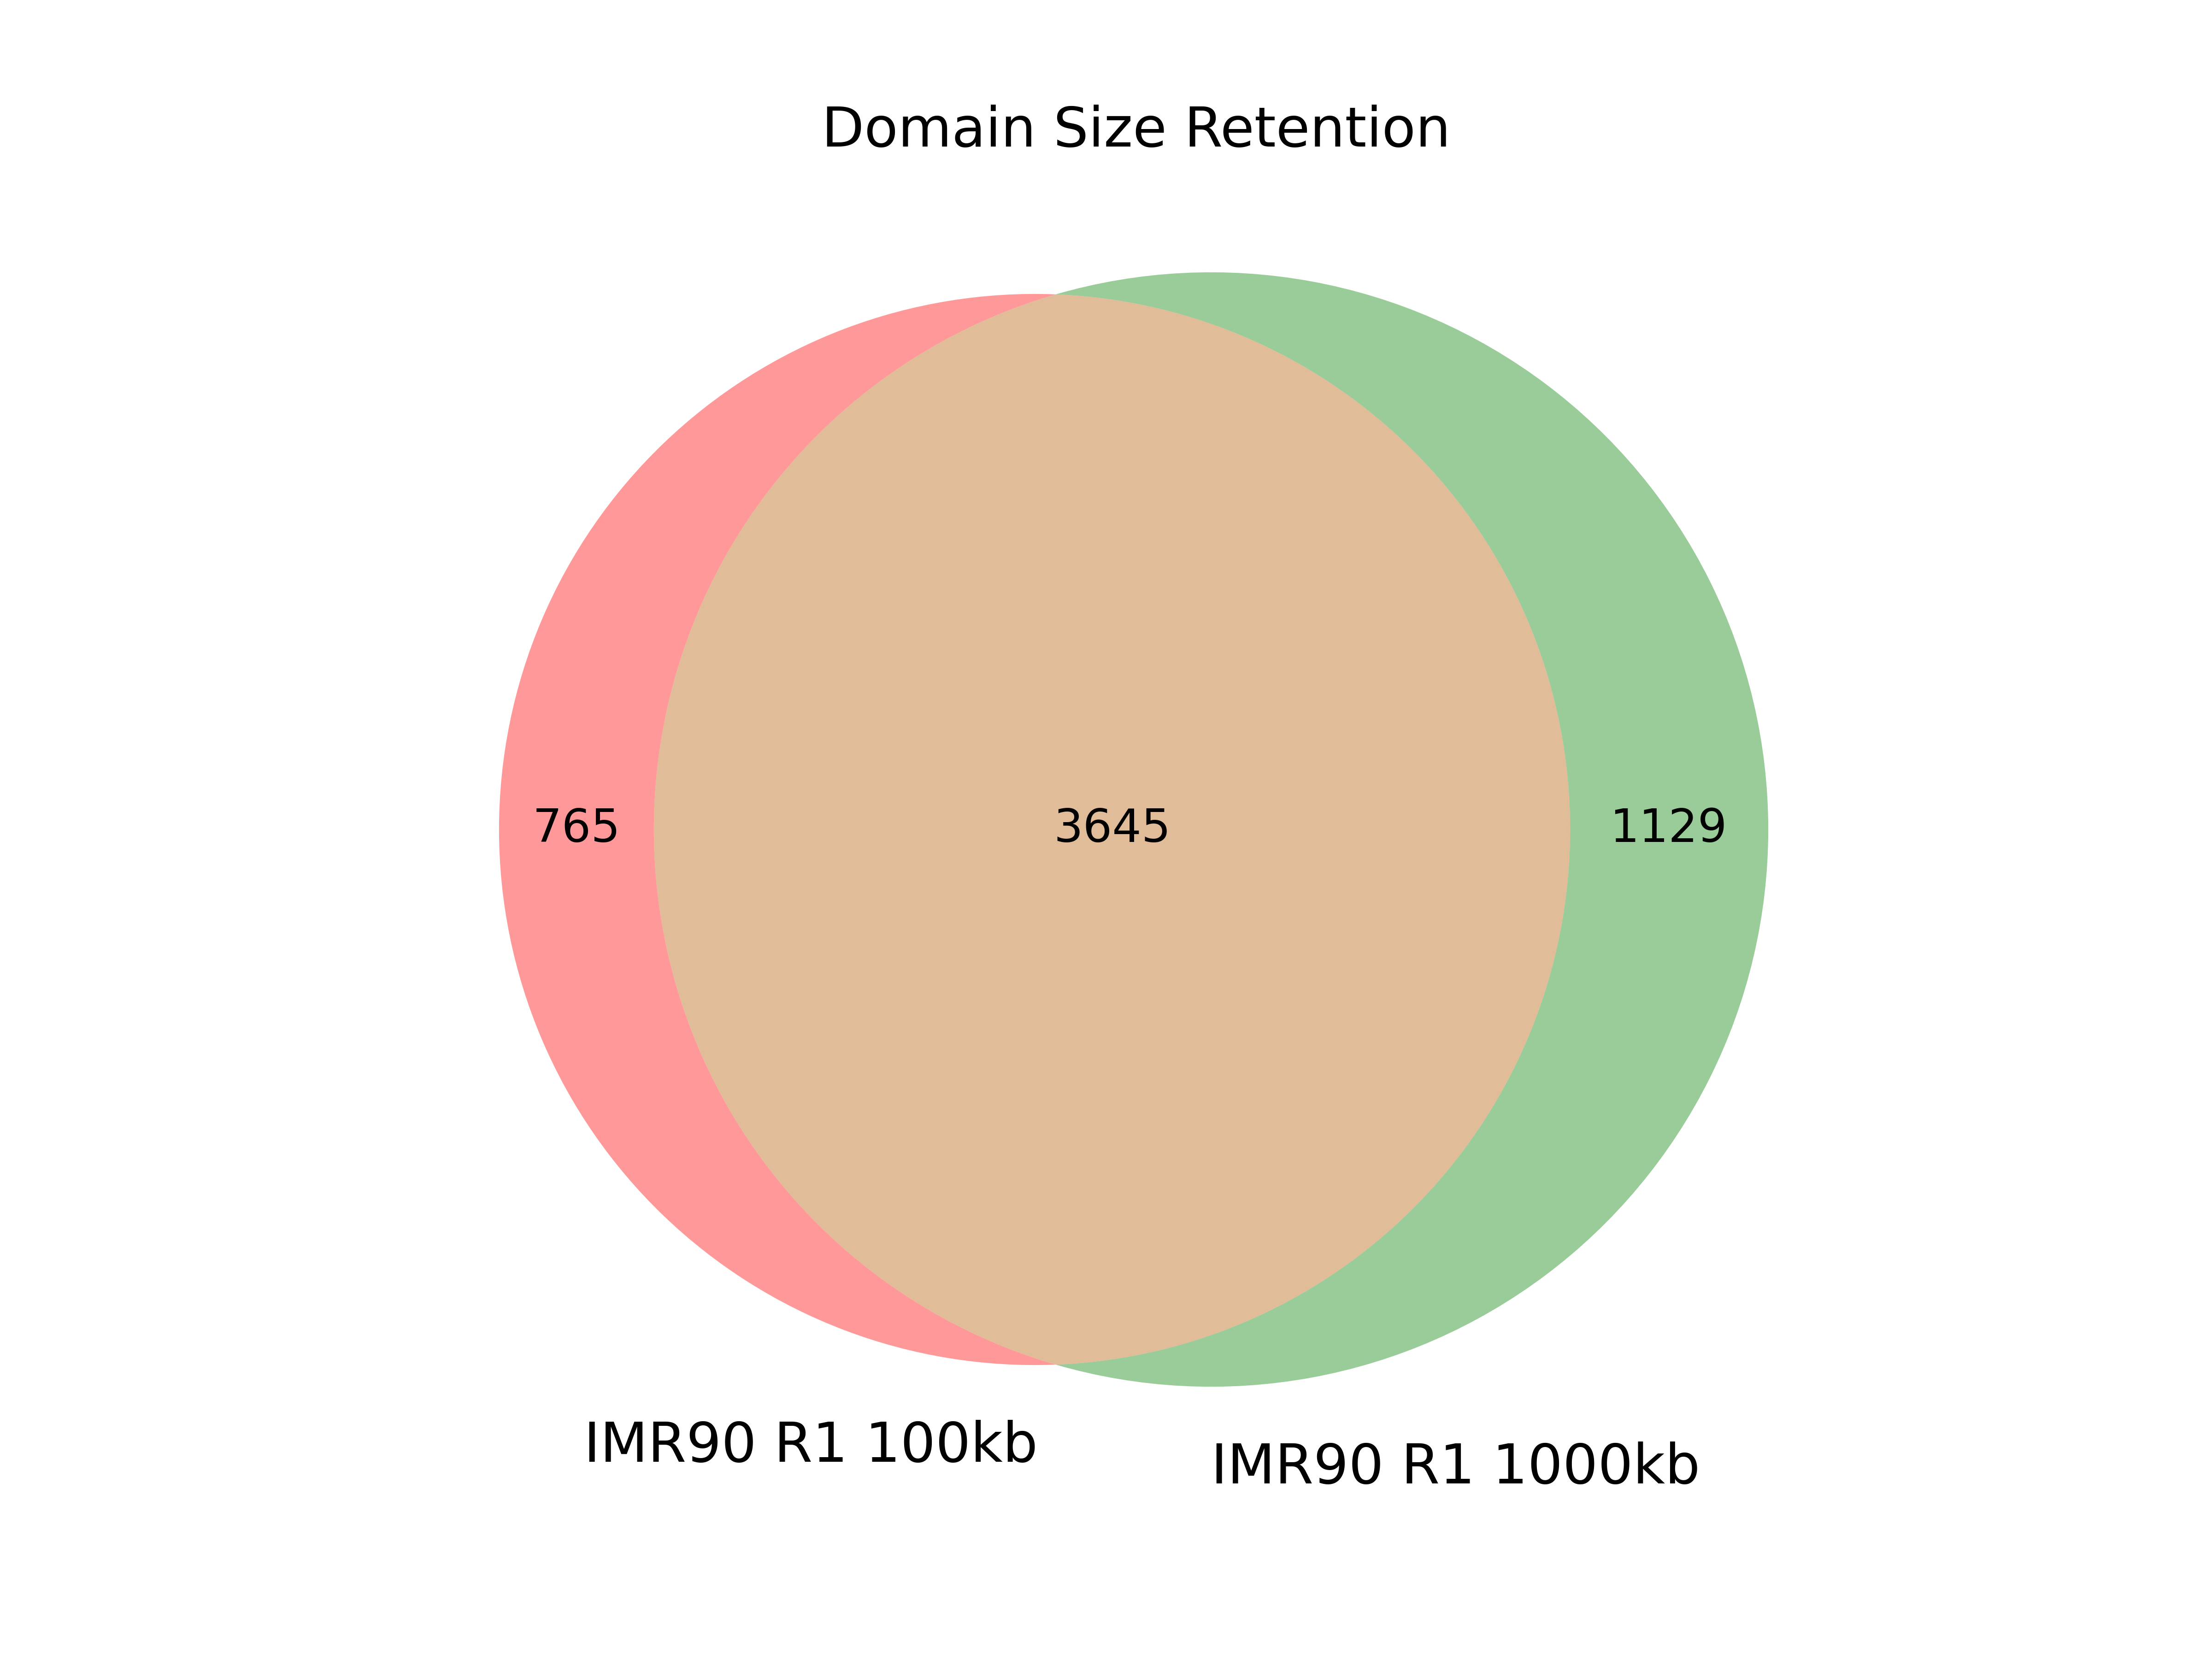
\includegraphics[width=\textwidth]{./figures/supplementary/domains/venn2_ir1_100kb_vs_ir1_1000kb.png}
  \end{minipage}

  \begin{minipage}{0.45\textwidth}
    \centering
    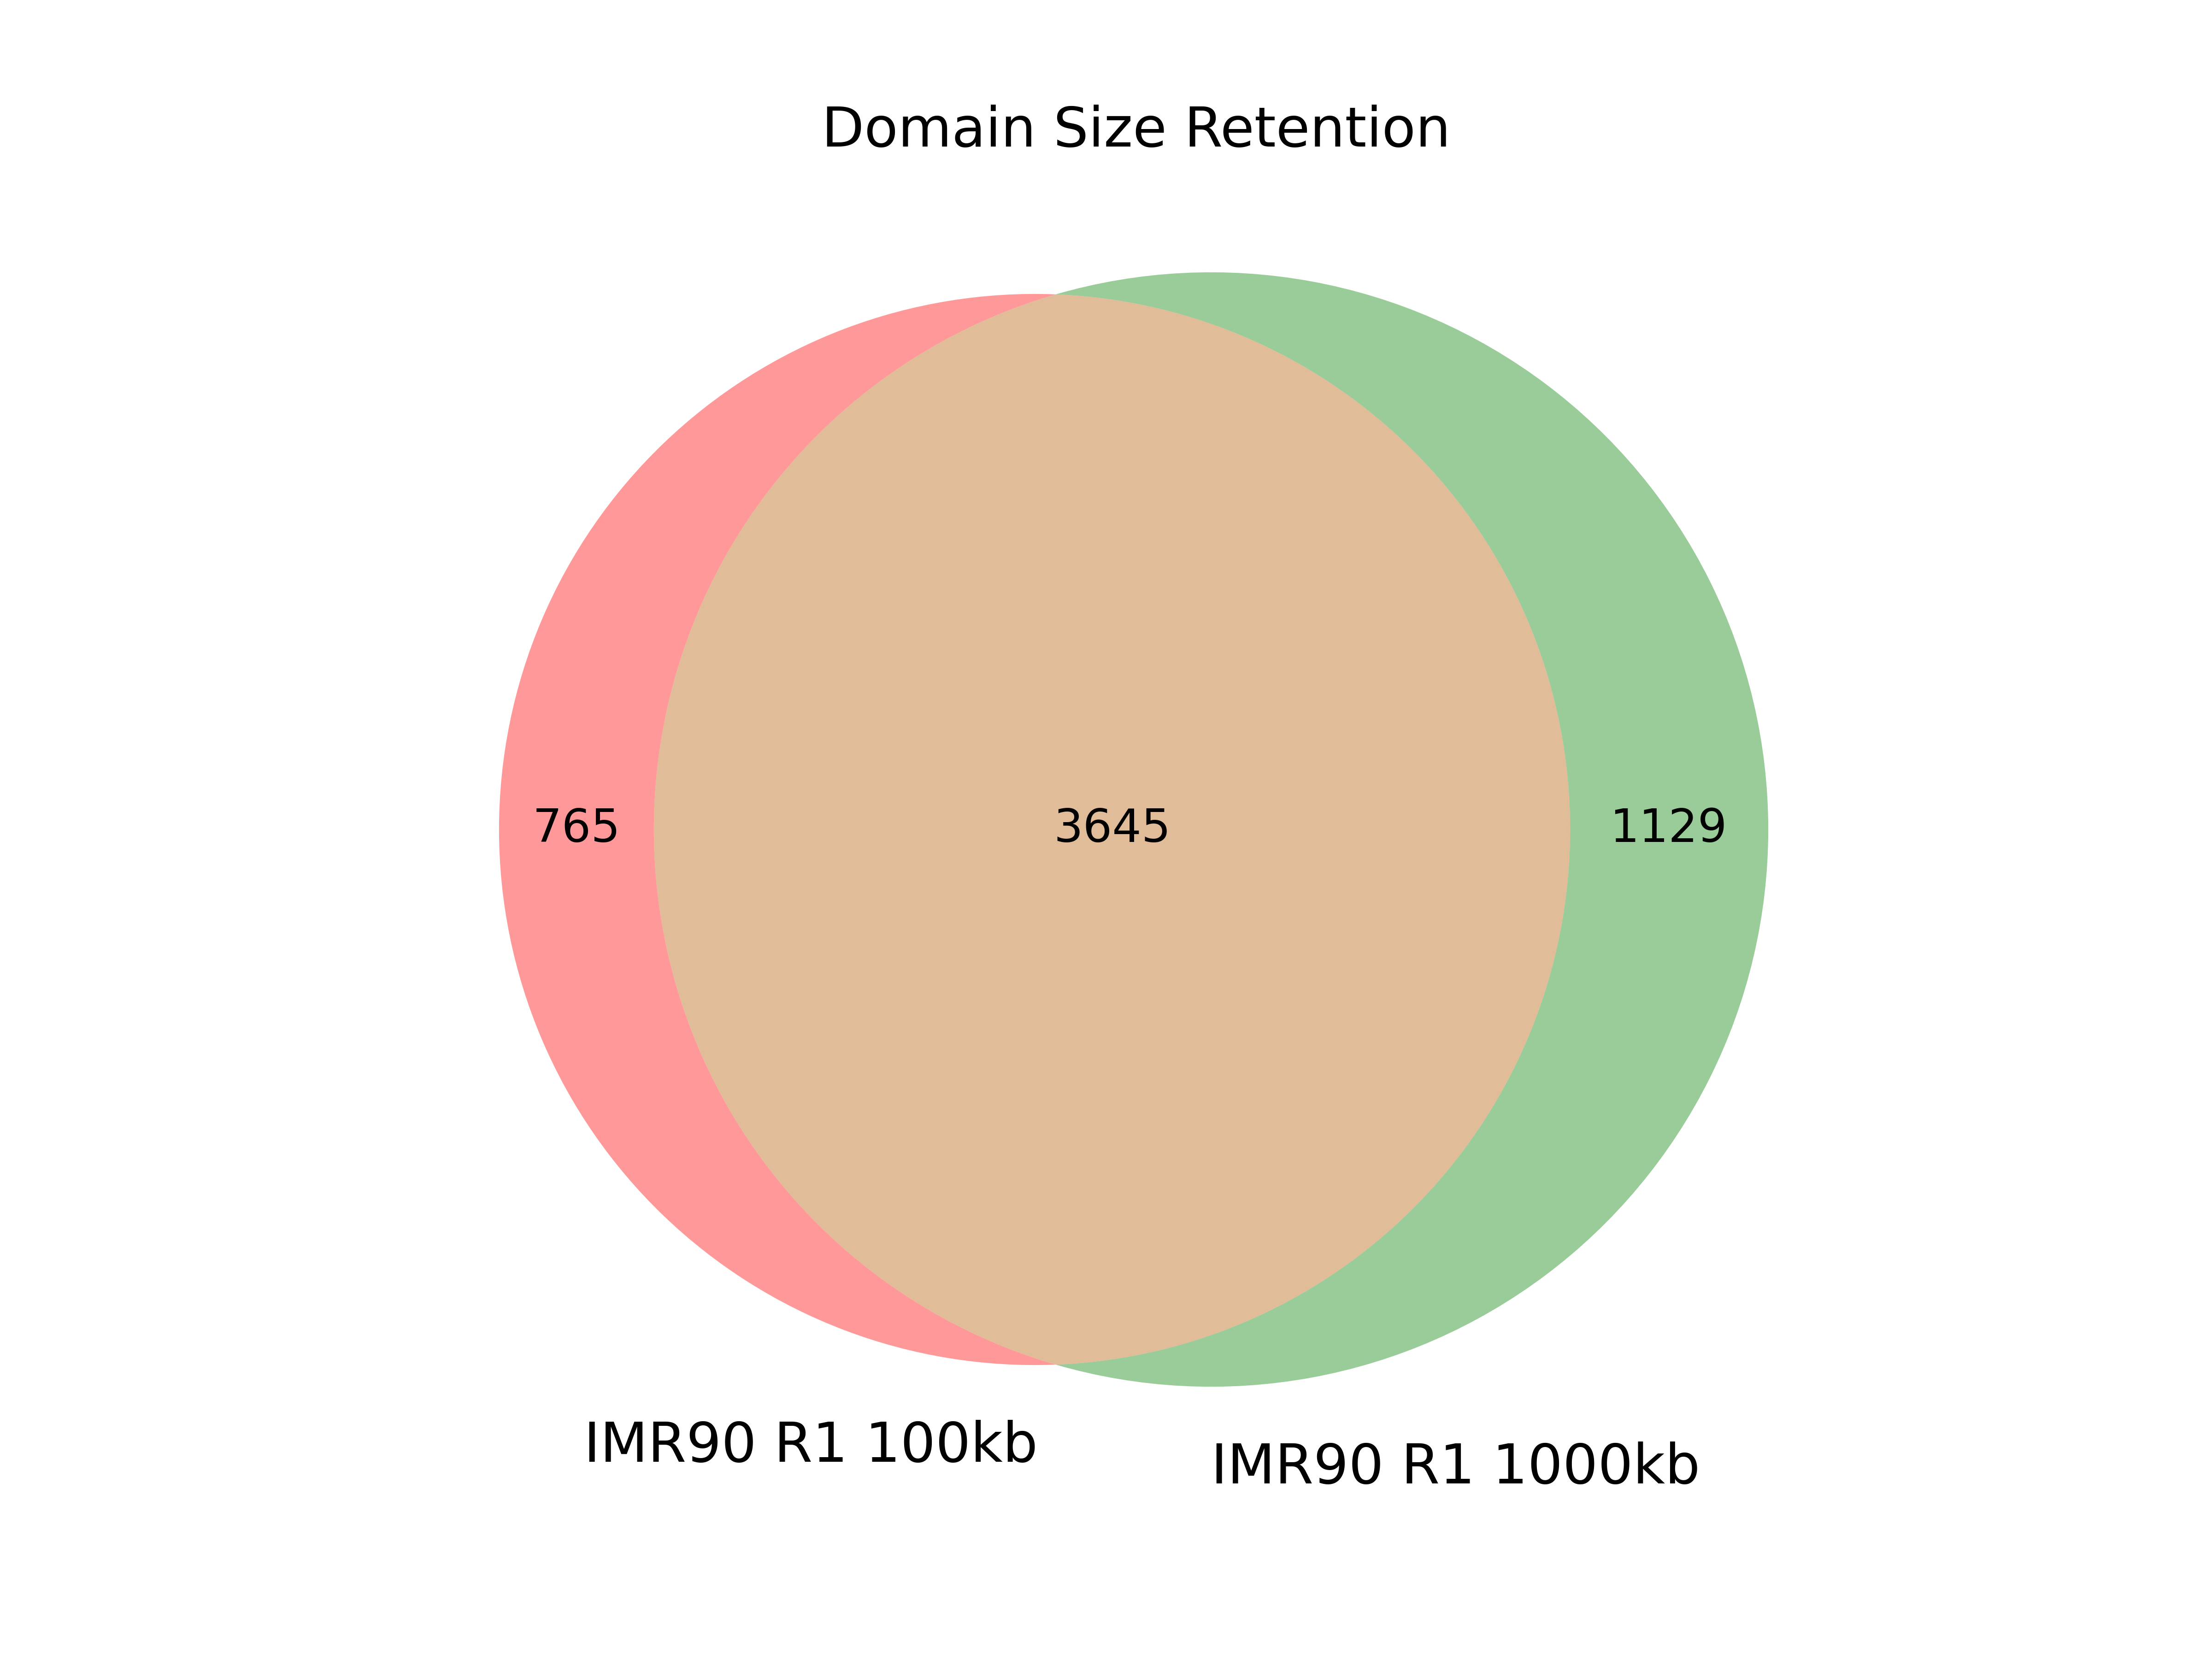
\includegraphics[width=\textwidth]{./figures/supplementary/domains/venn2_ir1_100kb_vs_ir1_1000kb.png}
  \end{minipage}
\end{figure}

\newpage

\subsection*{Domain Overlaps with Lesions}

\begin{figure}[thp]
  \centering
  \caption{Domain Overlaps by Window Size}
  \begin{minipage}{0.45\textwidth}%
    \centering
    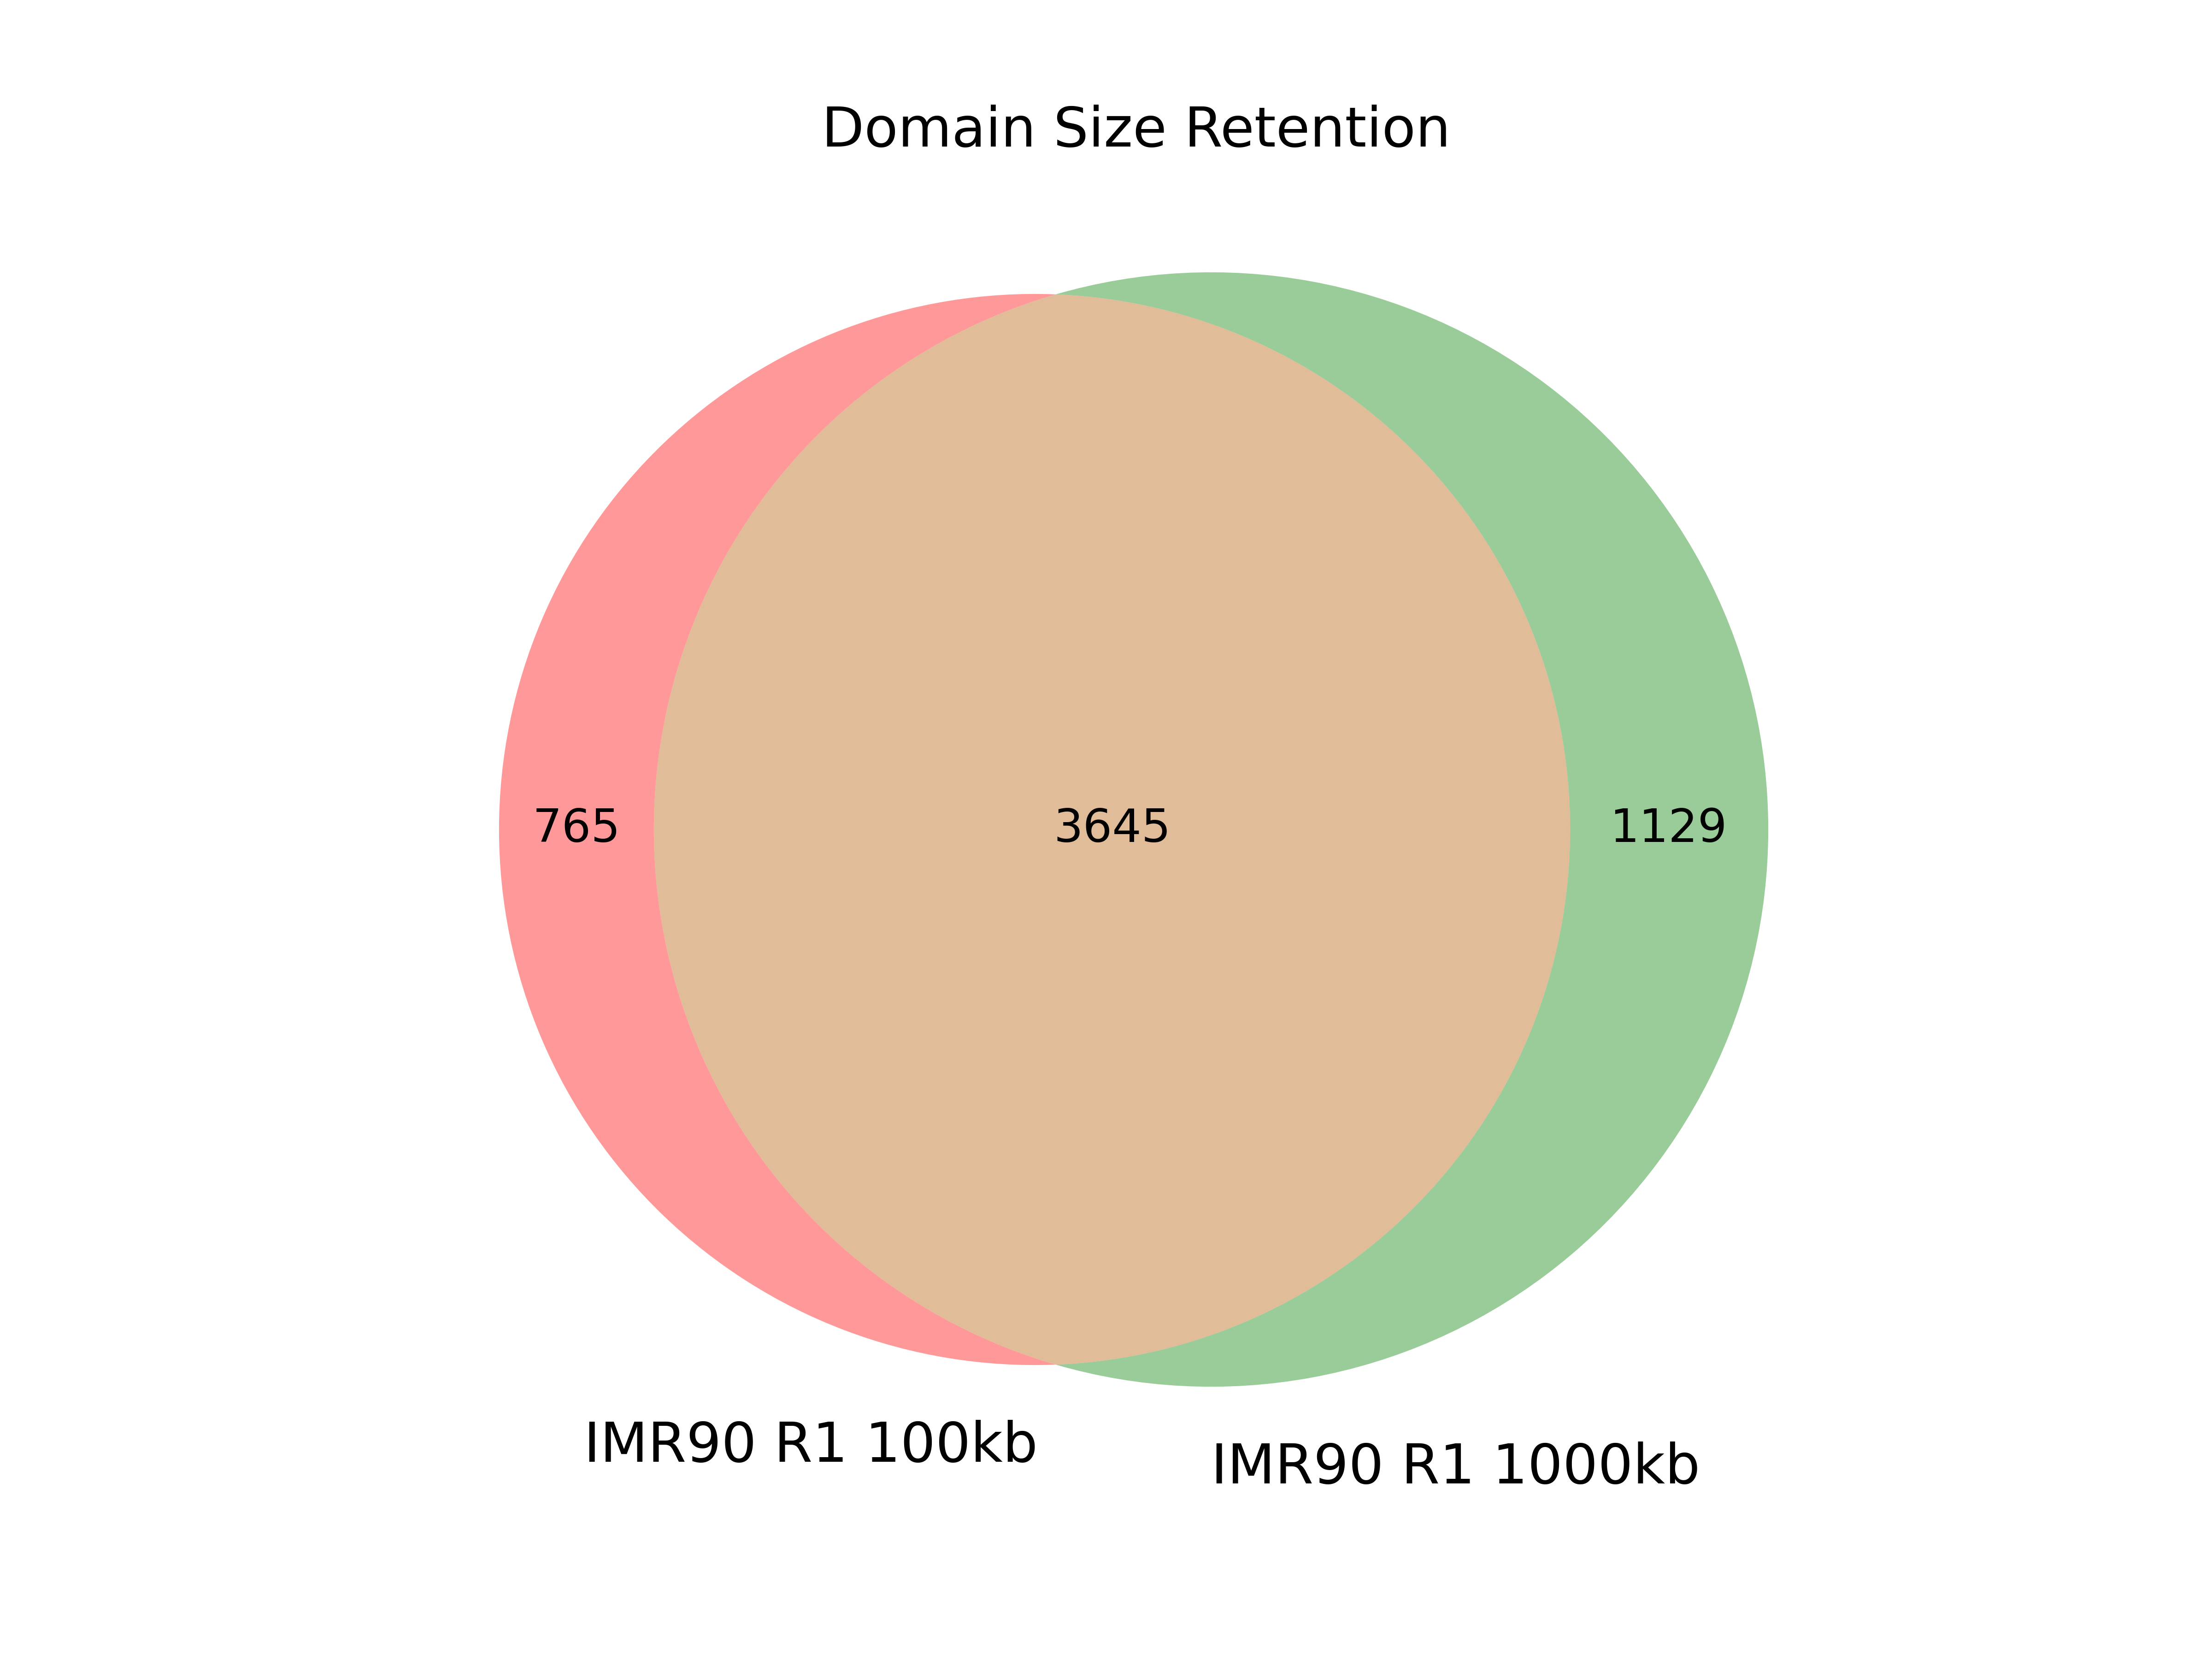
\includegraphics[width=\textwidth]{./figures/supplementary/domains/venn2_ir1_100kb_vs_ir1_1000kb.png}
  \end{minipage}

  \hfill

  \begin{minipage}{0.45\textwidth}
    \centering
    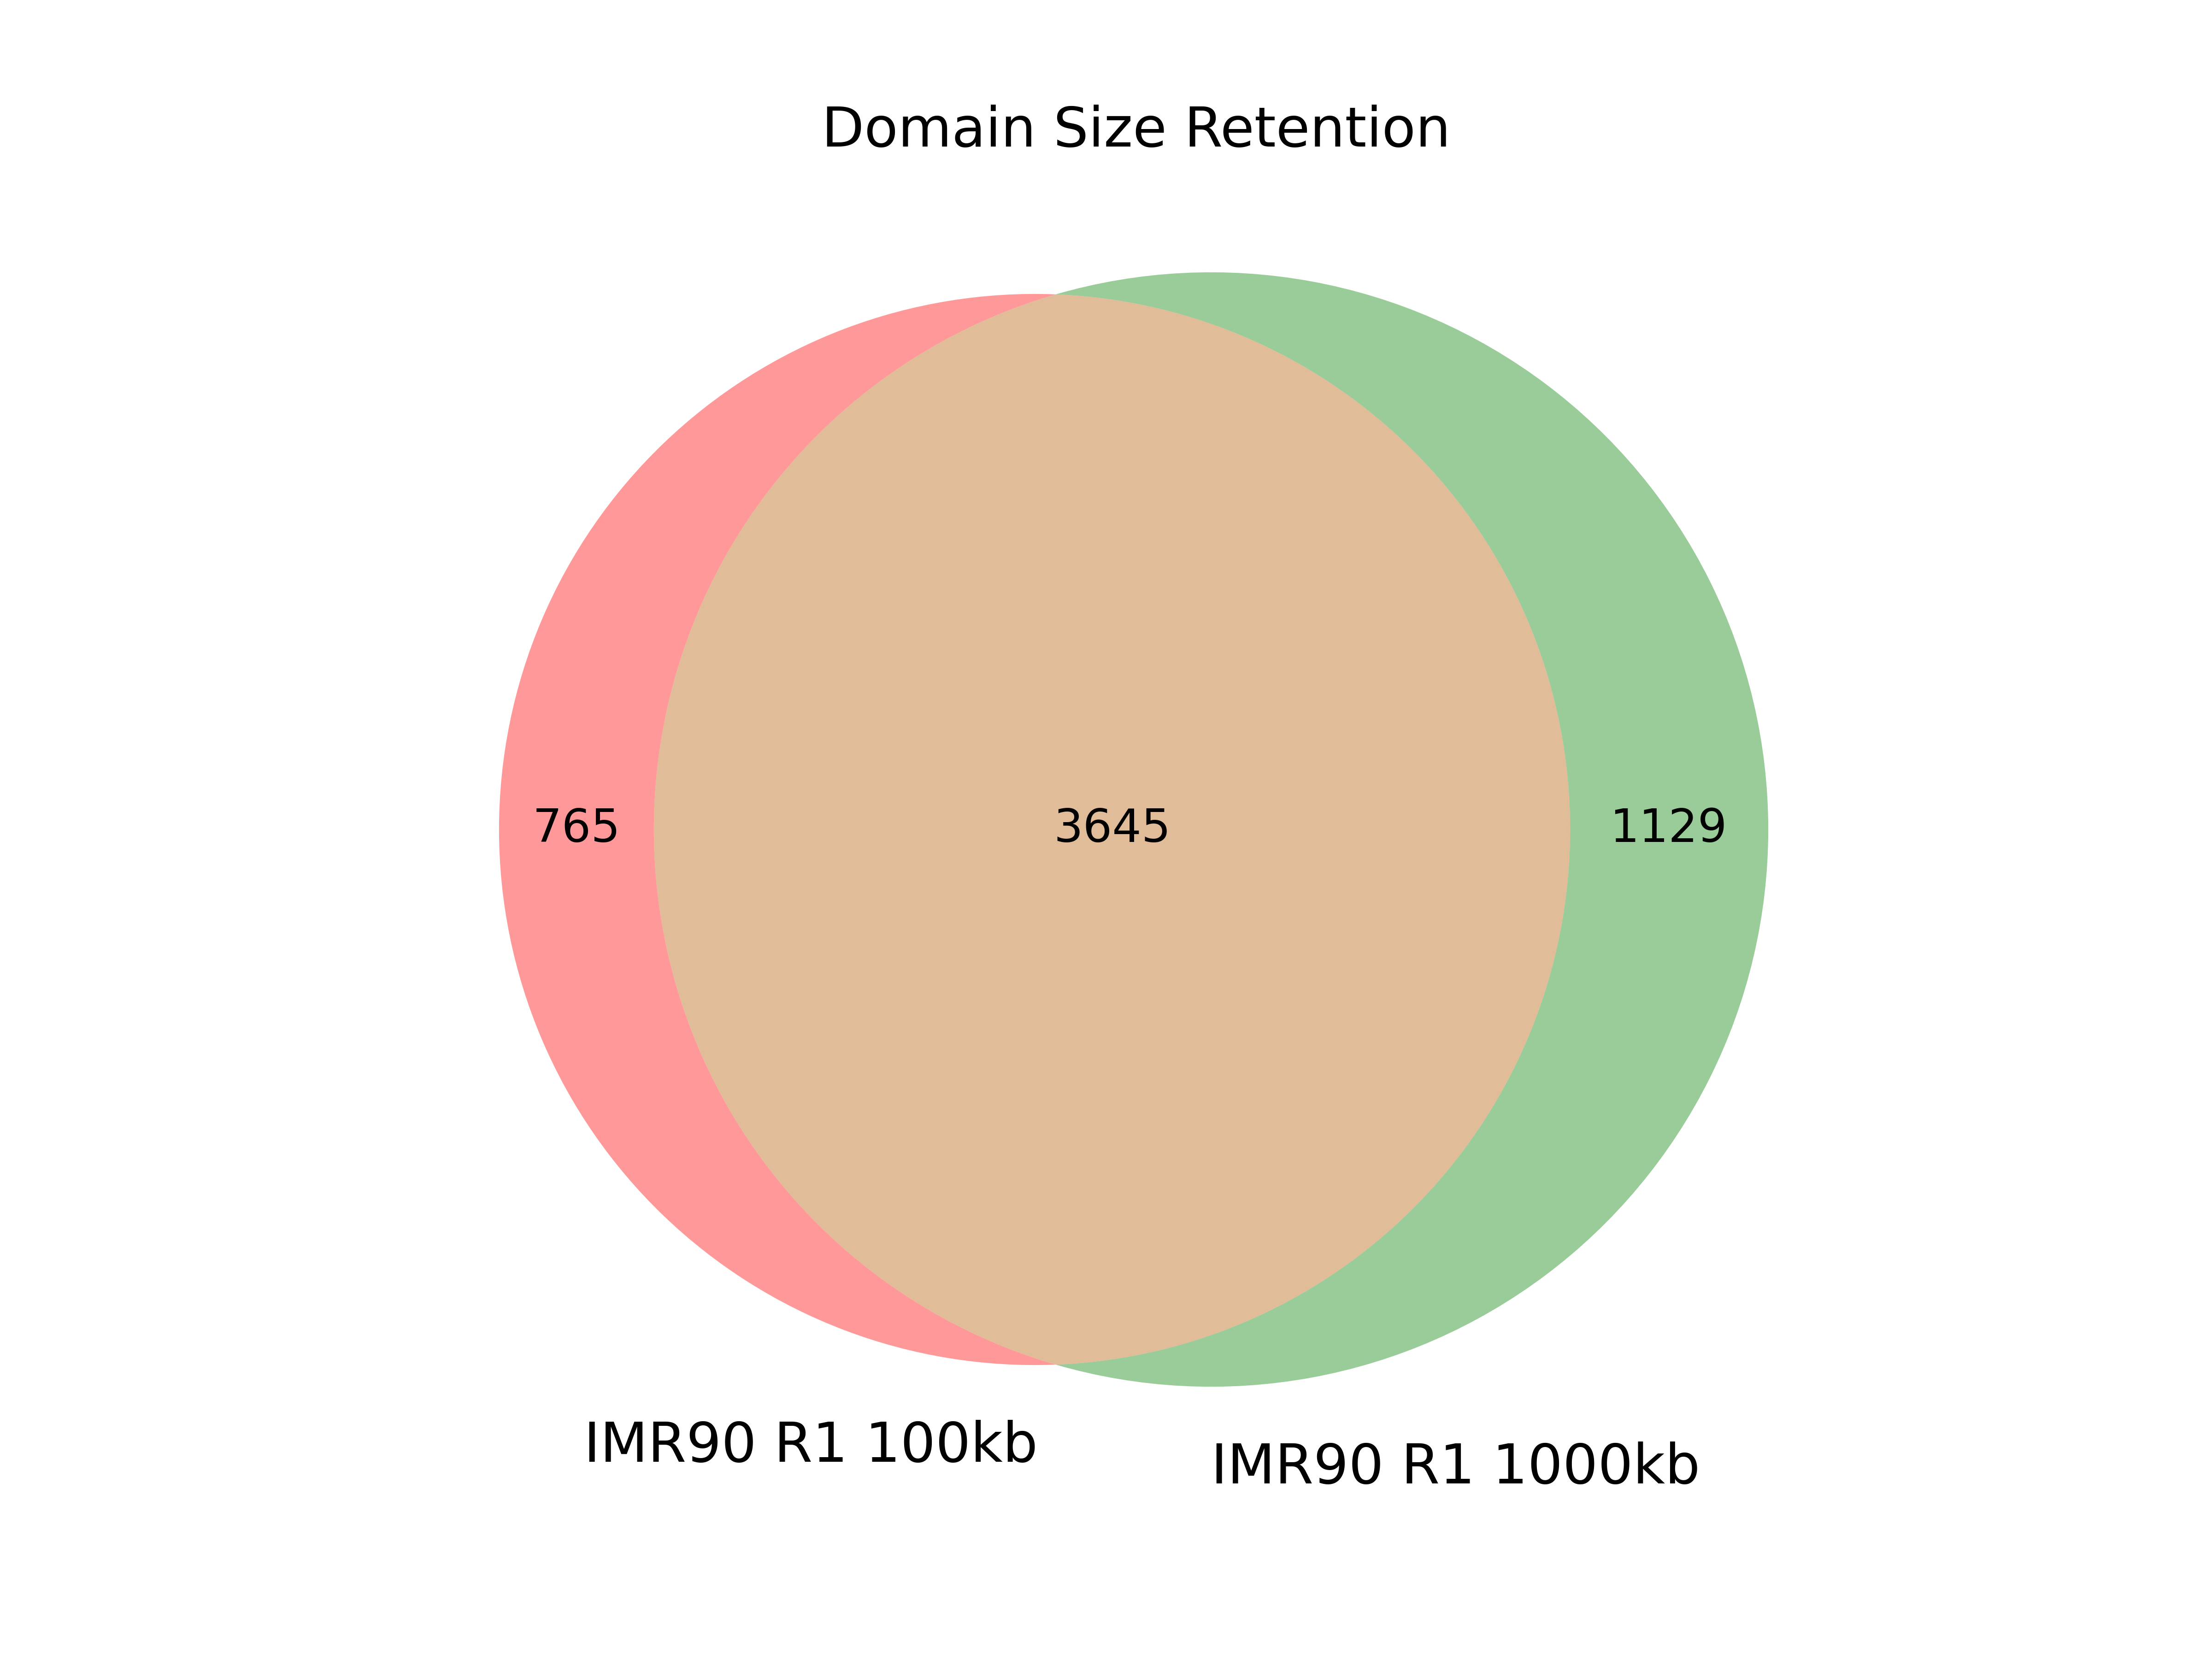
\includegraphics[width=\textwidth]{./figures/supplementary/domains/venn2_ir1_100kb_vs_ir1_1000kb.png}
  \end{minipage}
\end{figure}

\newpage
\section*{Biomarker Discovery}

\begin{figure}[H]
  \caption{Biomarkers at Conserved 200kb and 400kb Domain Boundaries}\label{fig:boundaryBiomarkers}
  \begin{minipage}{0.5\textwidth}%
    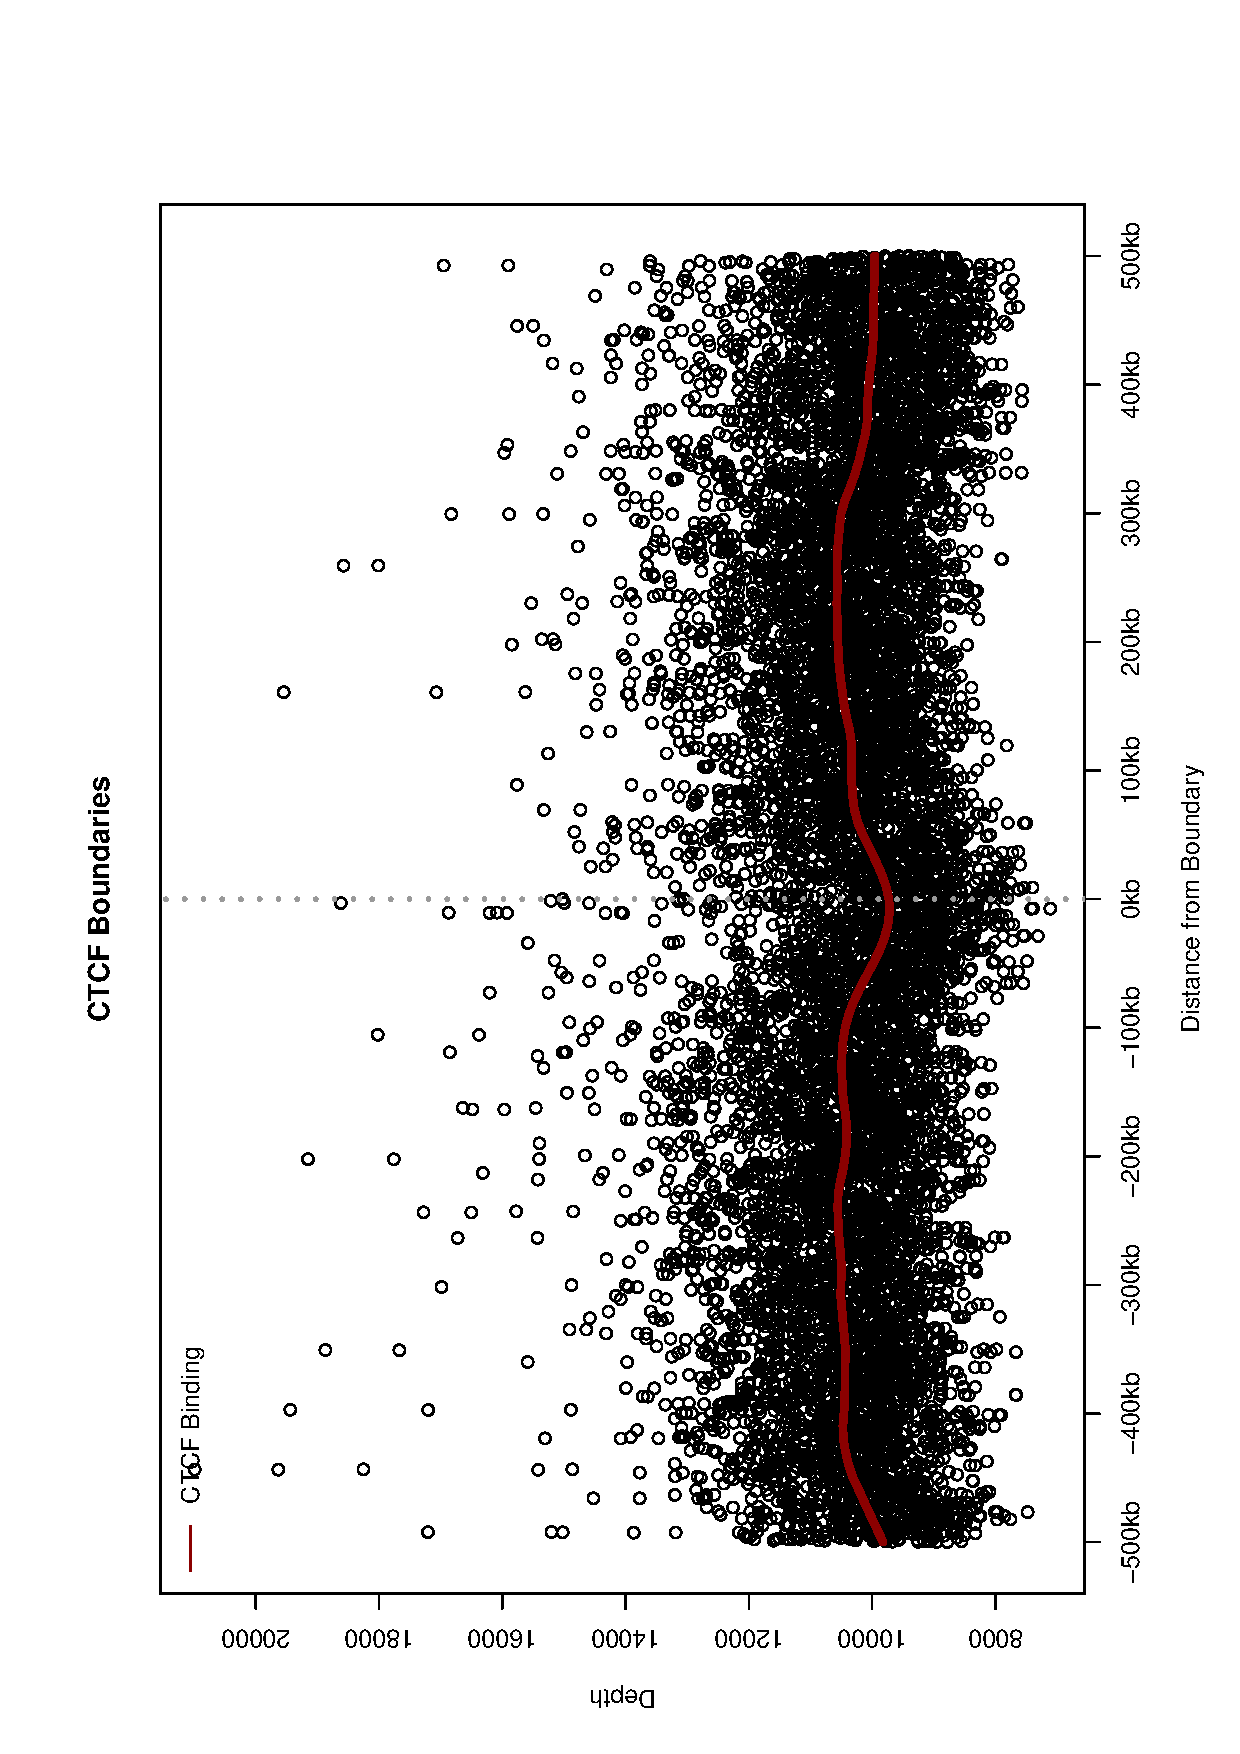
\includegraphics[width=\textwidth]{./figures/supplementary/biomarkers/ctcf200kbboundaries.pdf}
  \end{minipage}%
  \hfill
  \begin{minipage}{0.5\textwidth}
    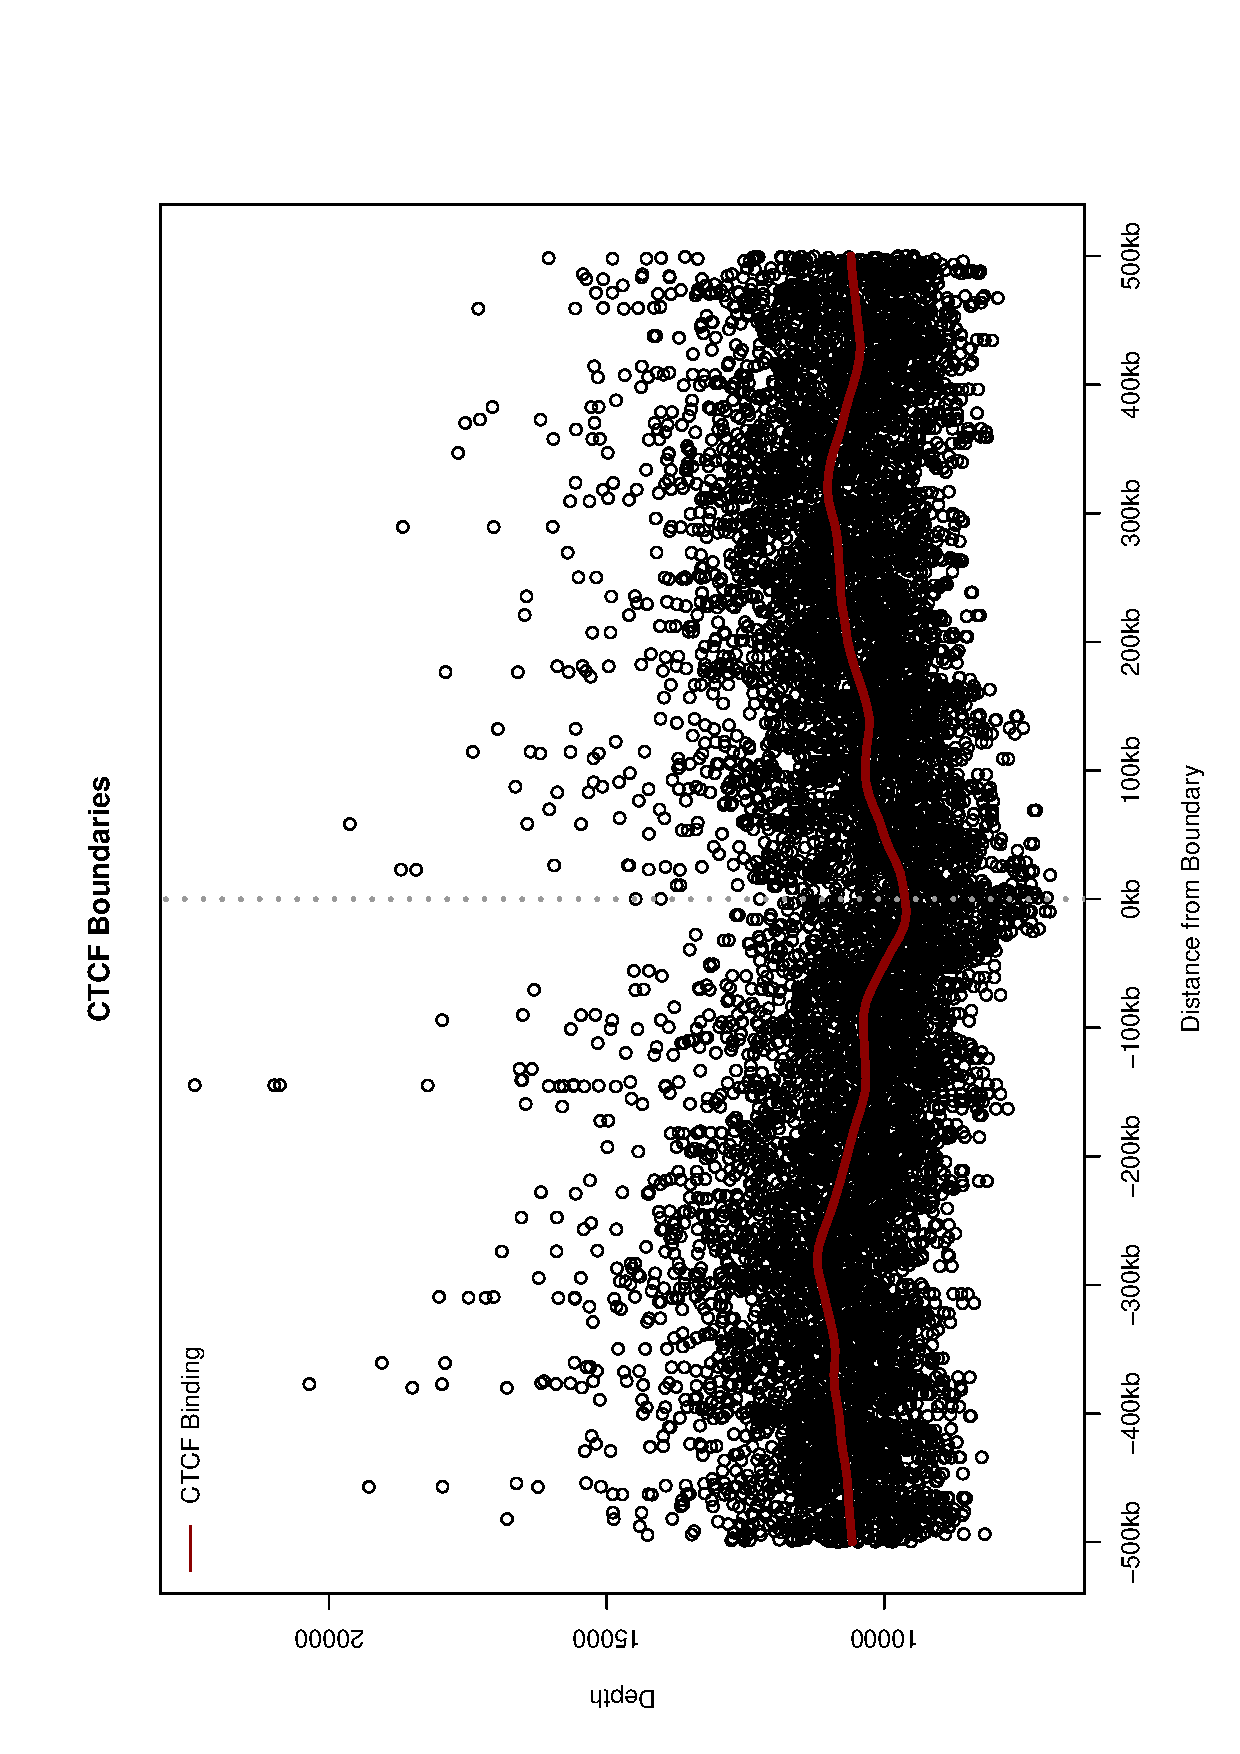
\includegraphics[width=\textwidth]{./figures/supplementary/biomarkers/ctcf400kbboundaries.pdf}
  \end{minipage}
\end{figure}

\begin{figure}[H]
  \begin{minipage}{0.5\textwidth}%
    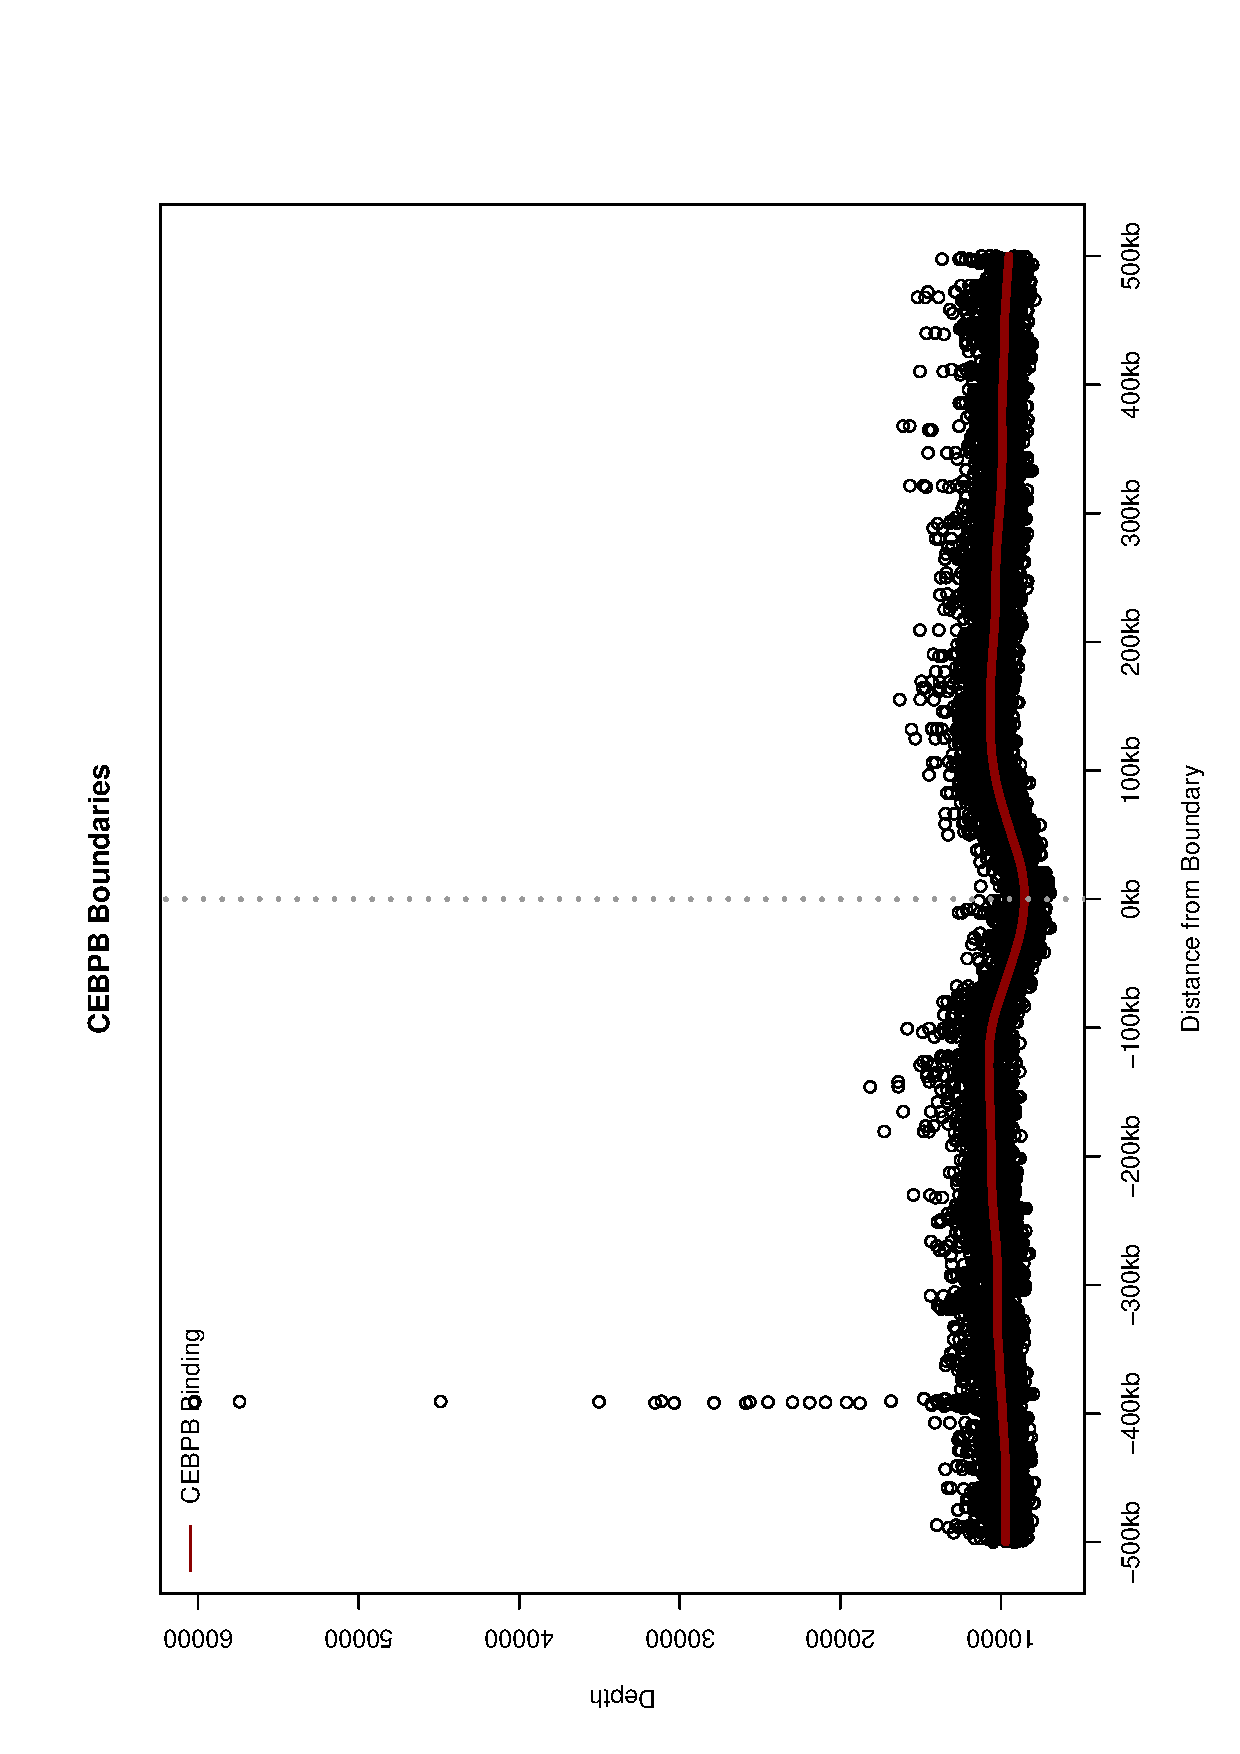
\includegraphics[width=\textwidth]{./figures/supplementary/biomarkers/cebpb200kbboundaries.pdf}
  \end{minipage}%
  \hfill
  \begin{minipage}{0.5\textwidth}
    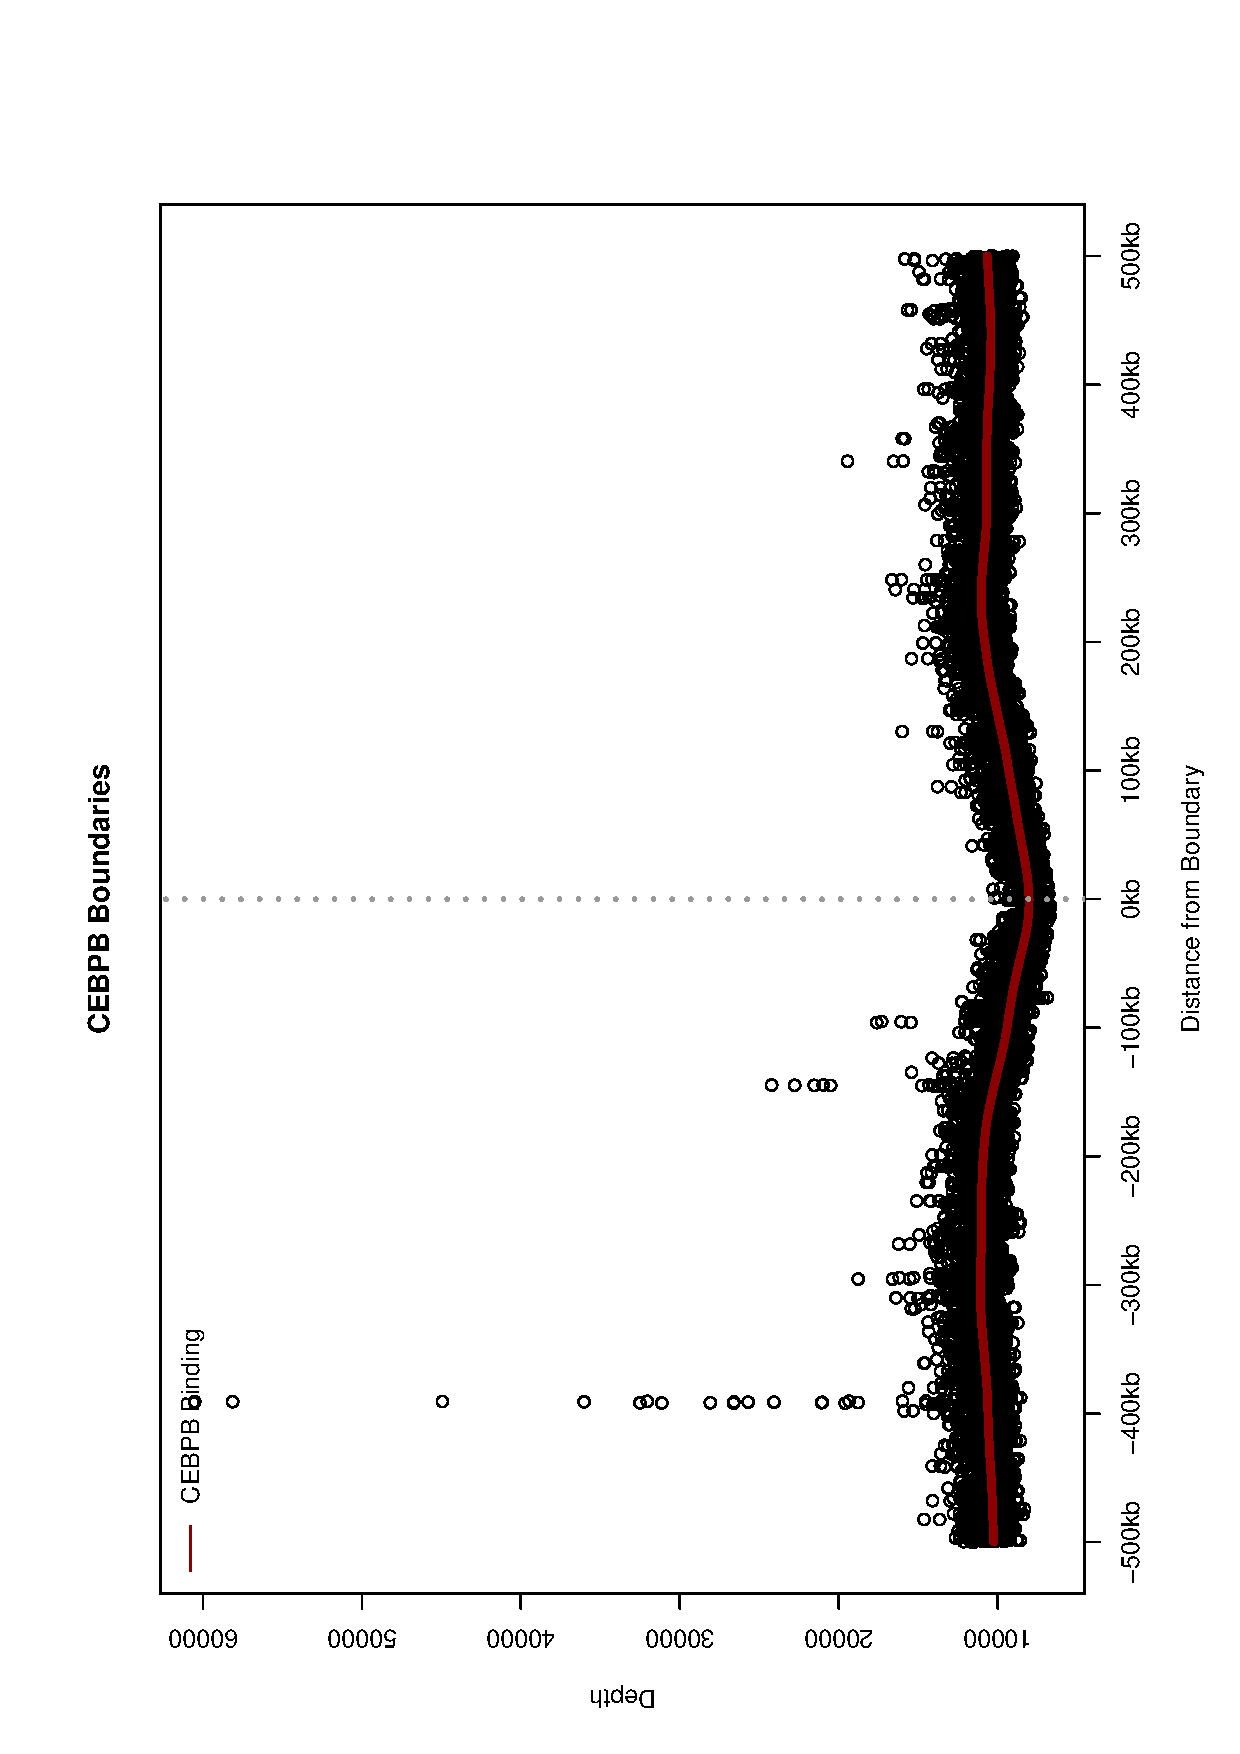
\includegraphics[width=\textwidth]{./figures/supplementary/biomarkers/cebpb400kbboundaries.pdf}
  \end{minipage}
\end{figure}

\begin{figure}[H]
  \begin{minipage}{0.5\textwidth}%
    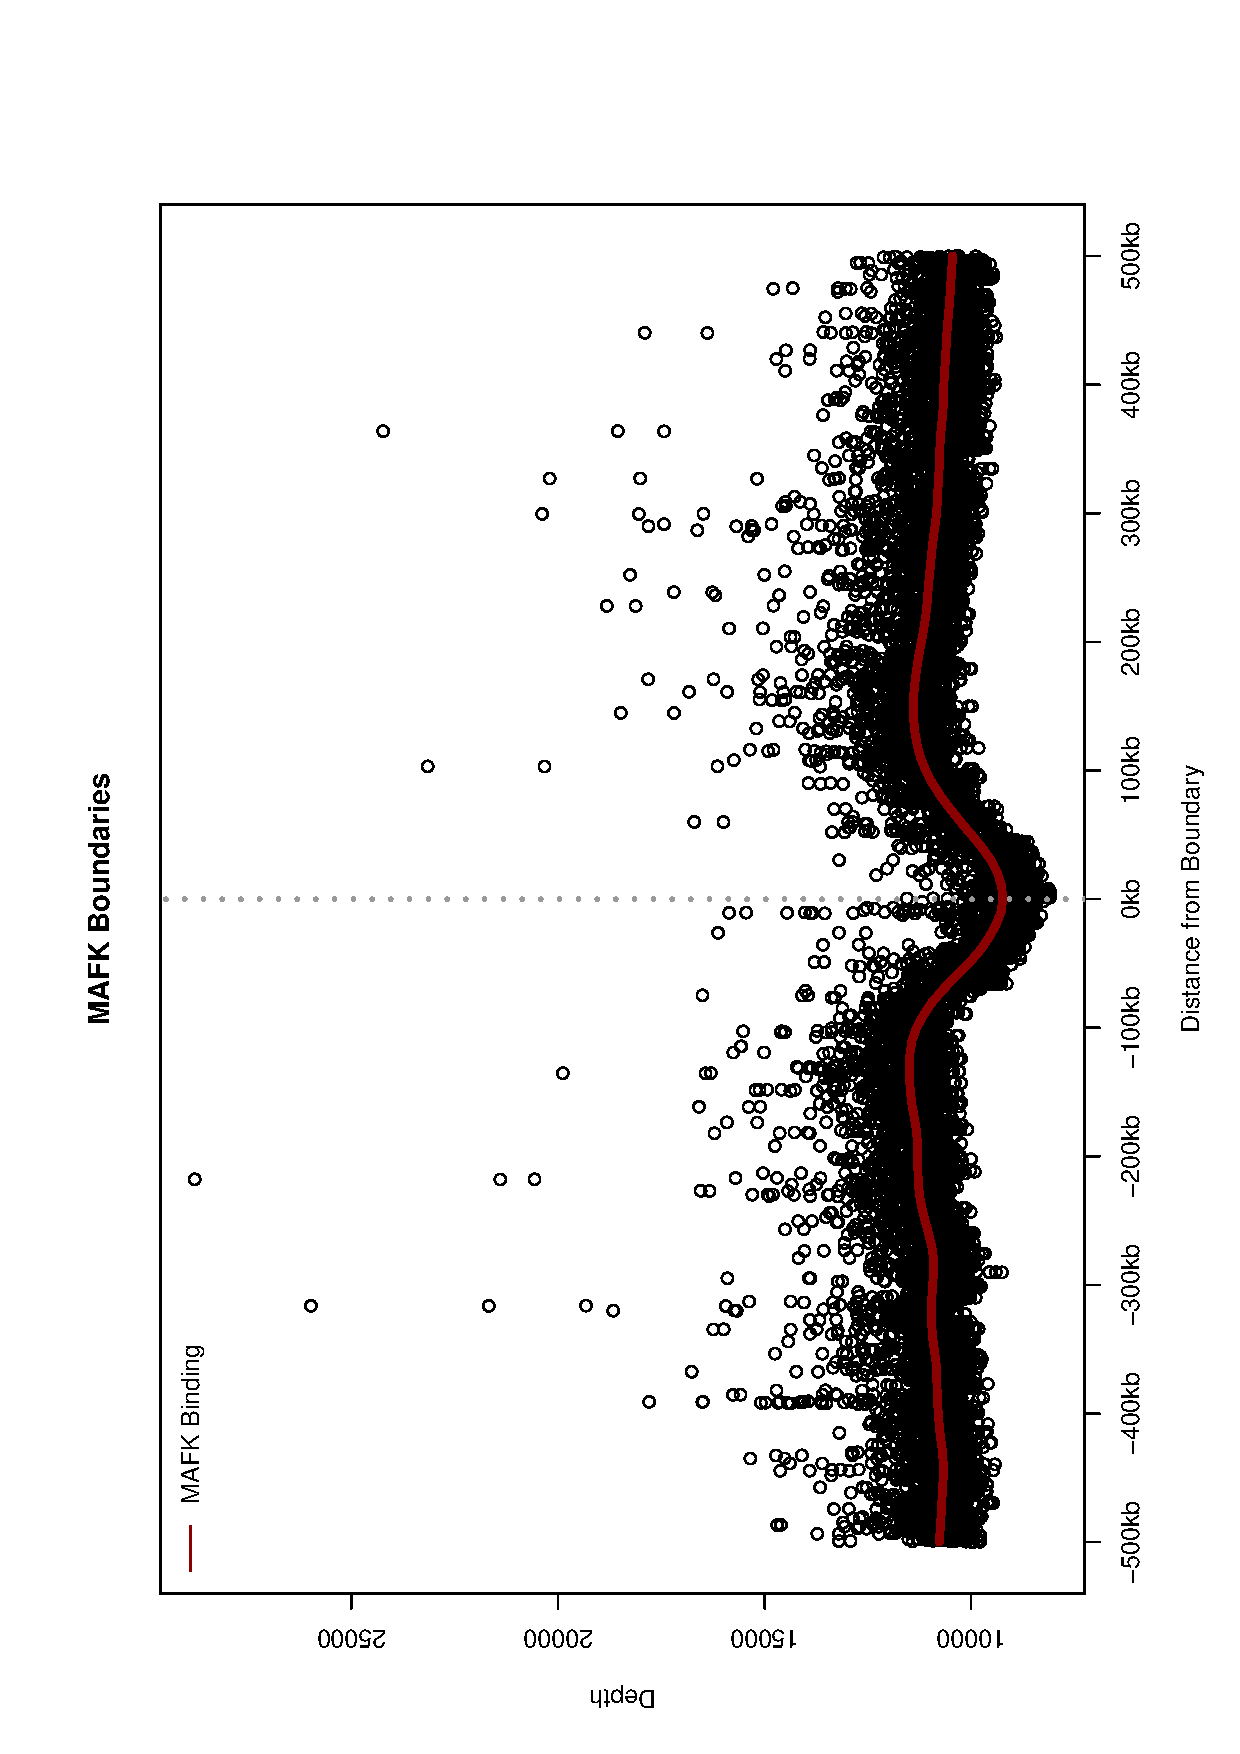
\includegraphics[width=\textwidth]{./figures/supplementary/biomarkers/mafk200kbboundaries.pdf}
  \end{minipage}%
  \hfill
  \begin{minipage}{0.5\textwidth}
    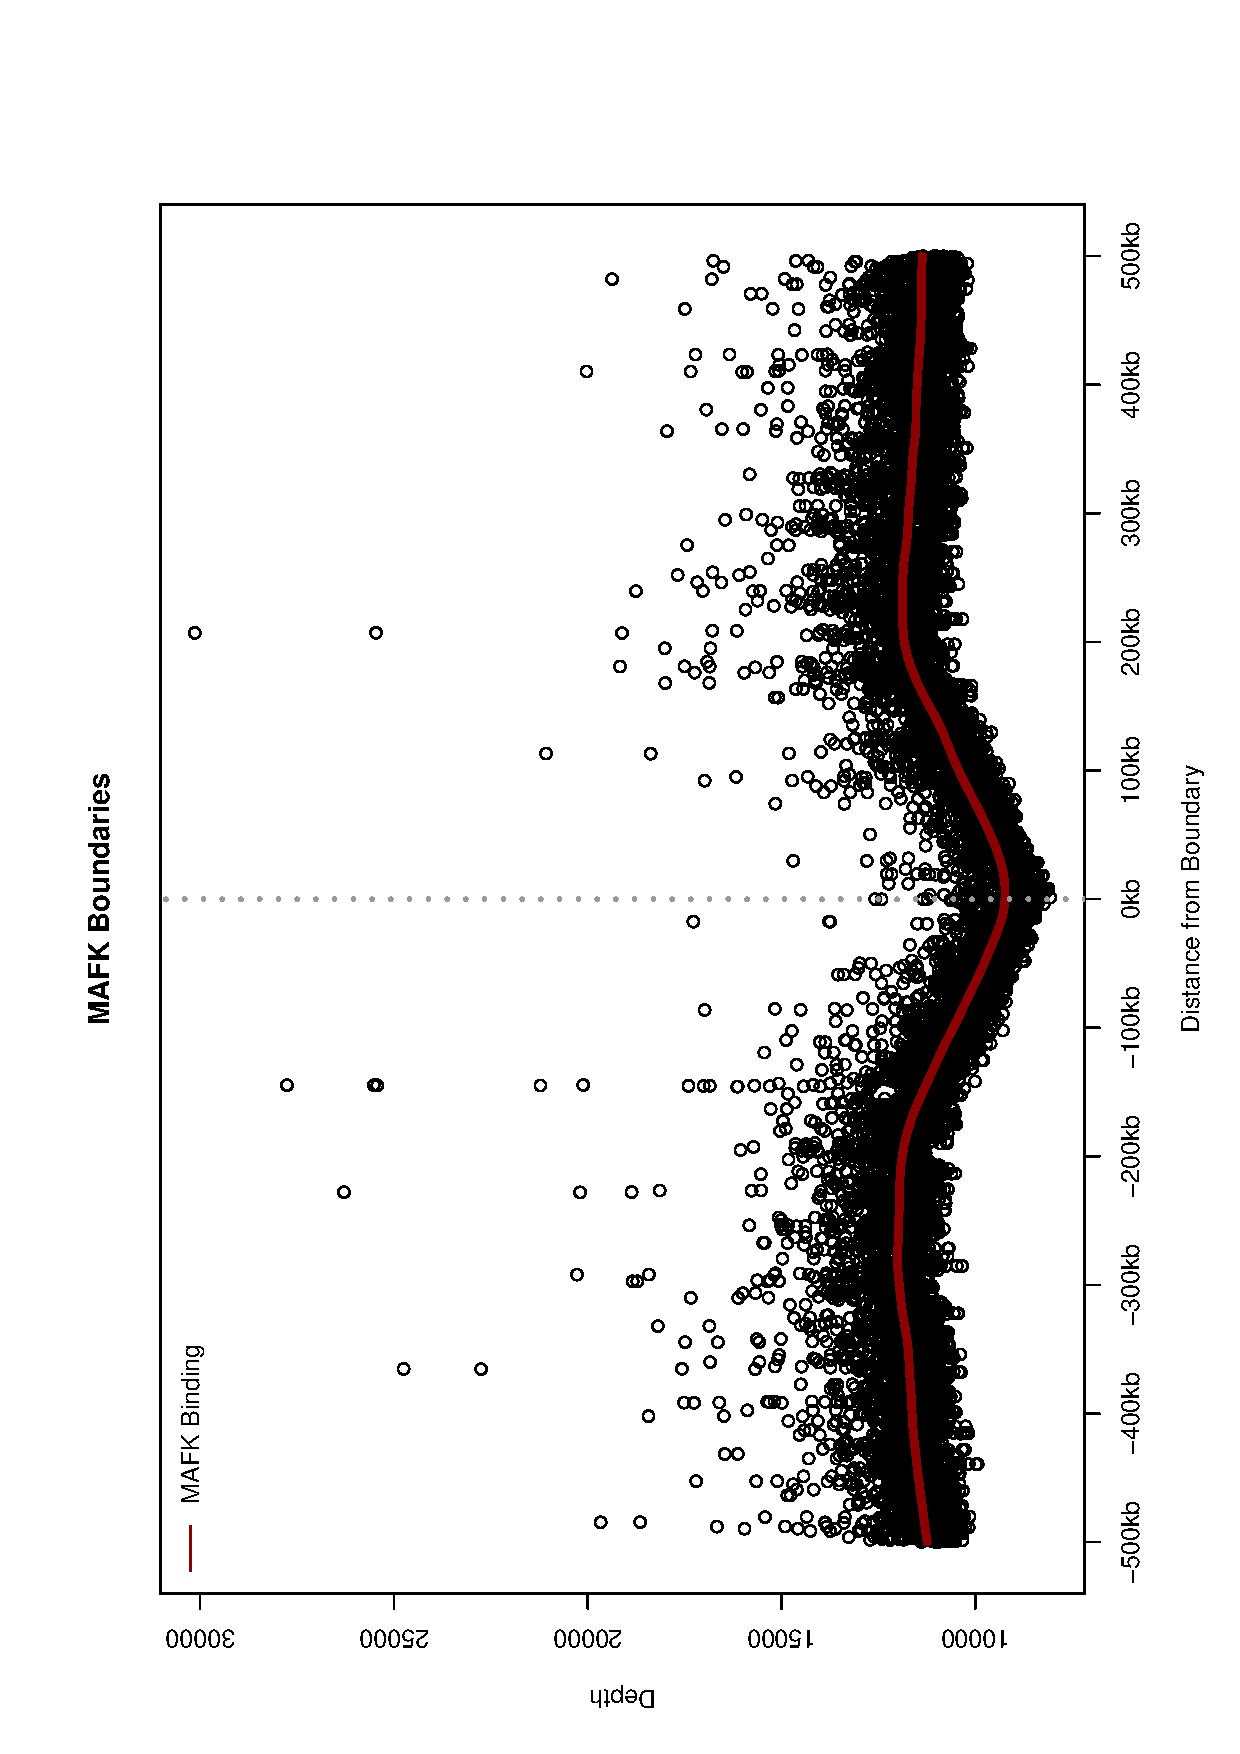
\includegraphics[width=\textwidth]{./figures/supplementary/biomarkers/mafk400kbboundaries.pdf}
  \end{minipage}
\end{figure}

\begin{figure}[H]
  \begin{minipage}{0.5\textwidth}%
    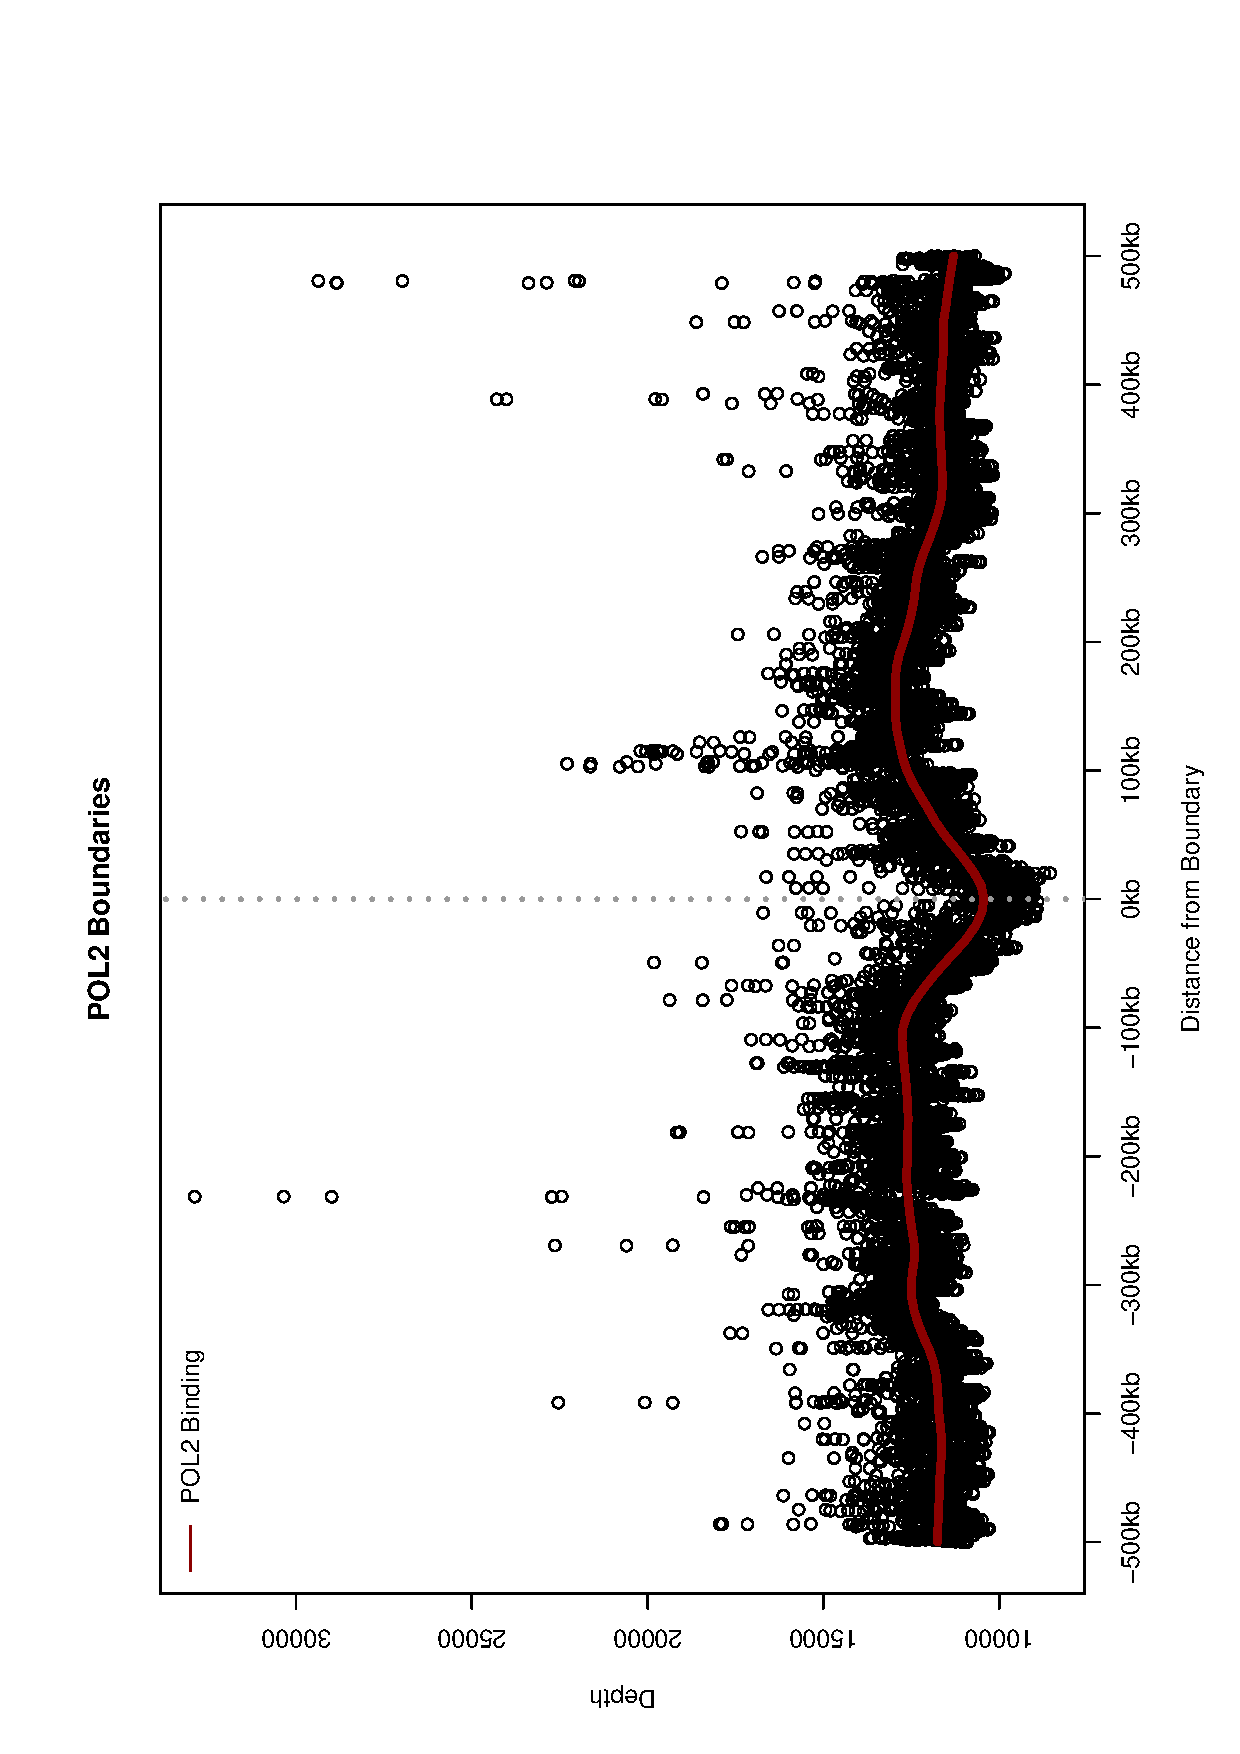
\includegraphics[width=\textwidth]{./figures/supplementary/biomarkers/pol2200kbboundaries.pdf}
  \end{minipage}%
  \hfill
  \begin{minipage}{0.5\textwidth}
    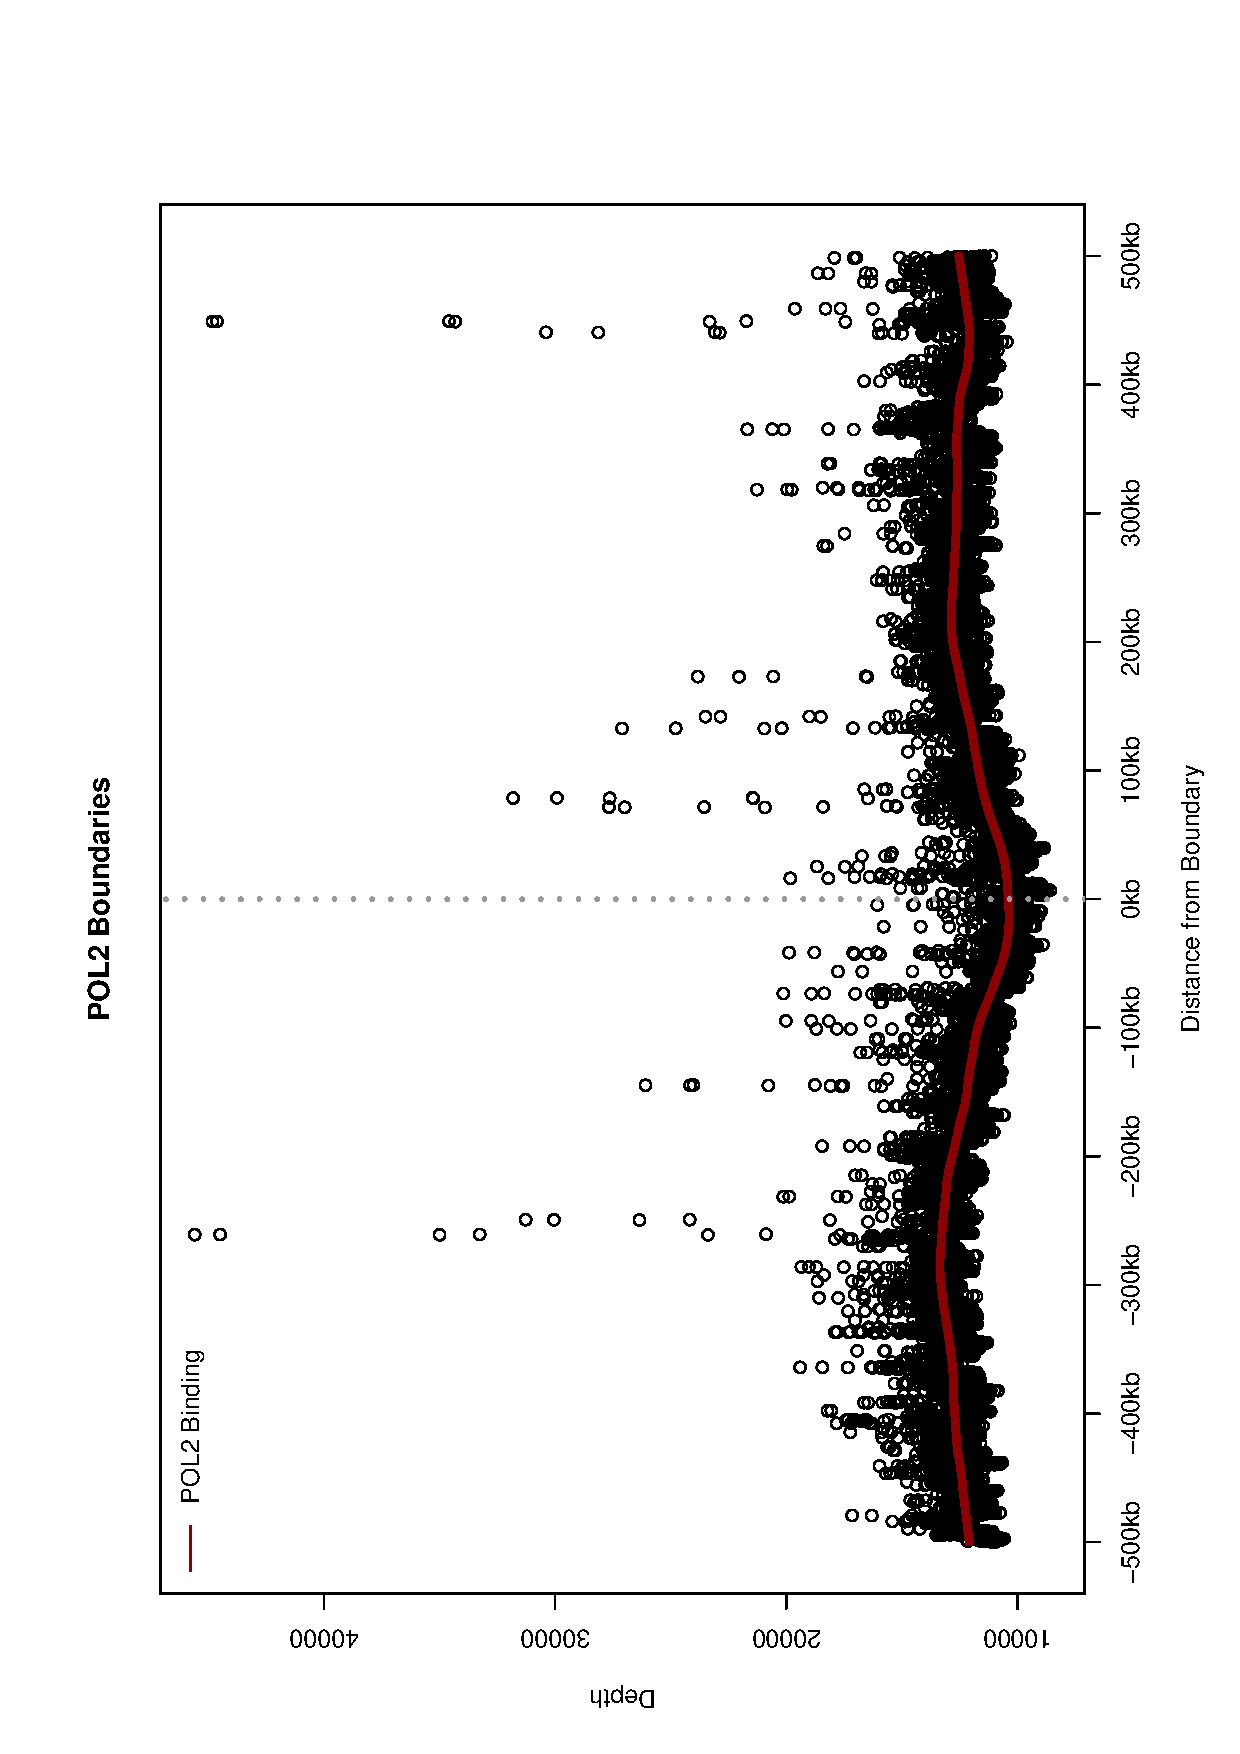
\includegraphics[width=\textwidth]{./figures/supplementary/biomarkers/pol2400kbboundaries.pdf}
  \end{minipage}
\end{figure}

\begin{figure}[H]
  \begin{minipage}{0.5\textwidth}%
    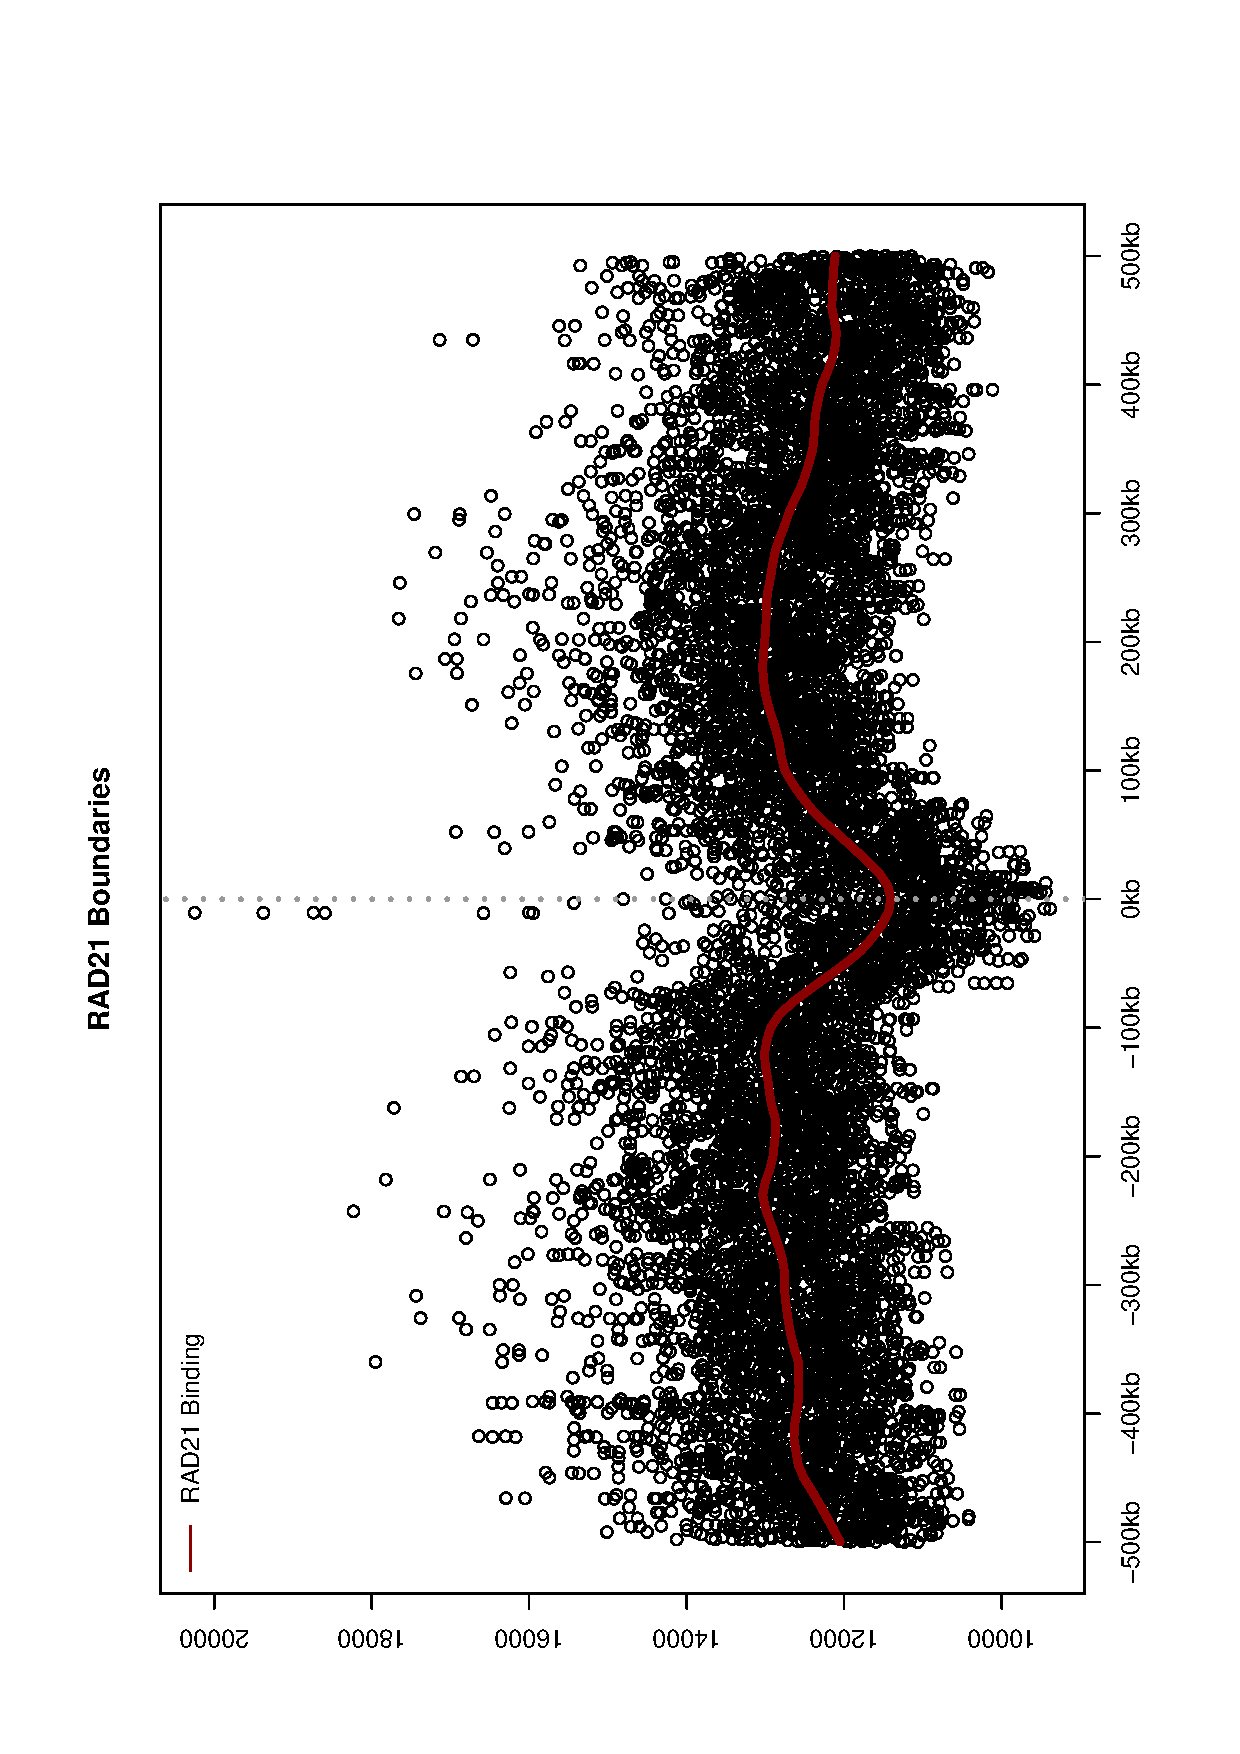
\includegraphics[width=\textwidth]{./figures/supplementary/biomarkers/rad21200kbboundaries.pdf}
  \end{minipage}%
  \hfill
  \begin{minipage}{0.5\textwidth}
    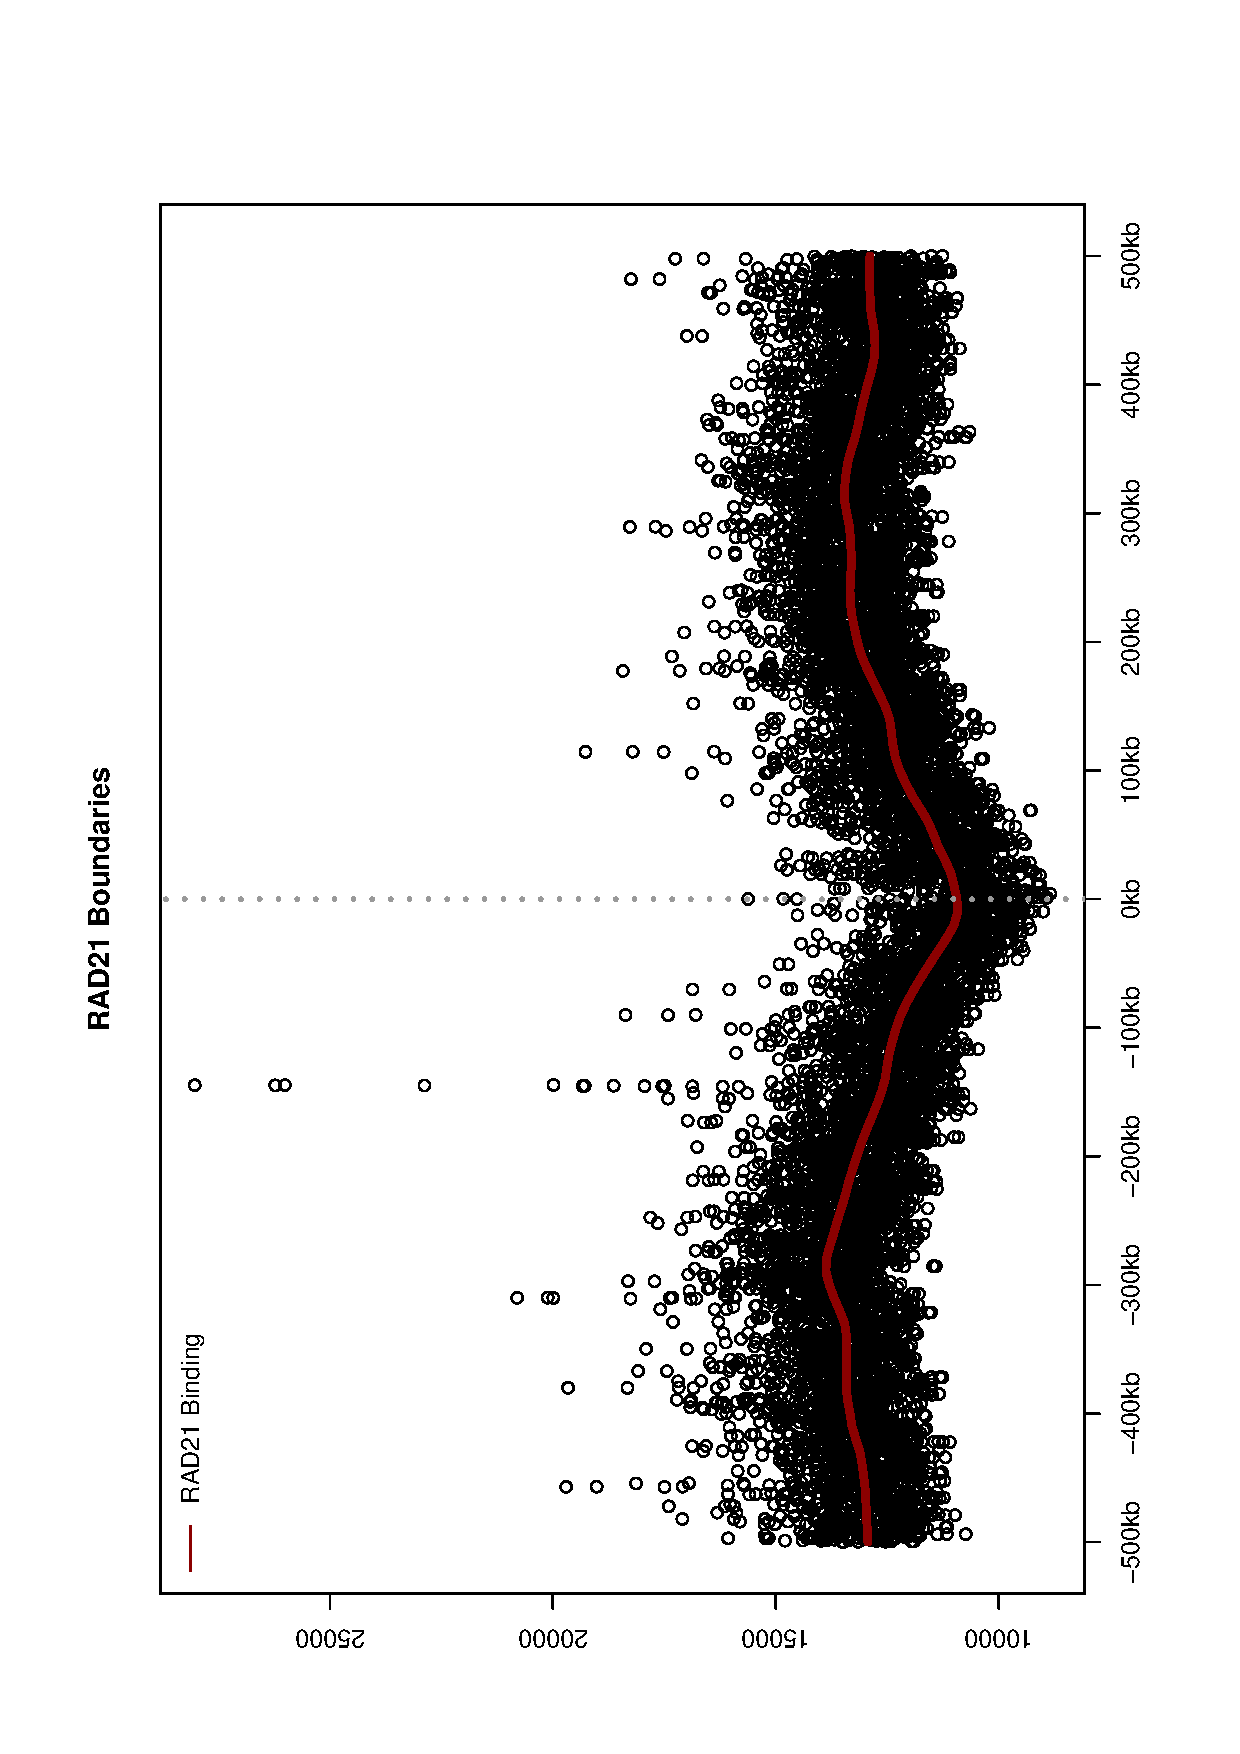
\includegraphics[width=\textwidth]{./figures/supplementary/biomarkers/rad21400kbboundaries.pdf}
  \end{minipage}
  \medskip
  \small
  Binding of various biomarkers around domain boundaries.  Using domains discovered at 200kb (left) and 400kb (right)
  \gls{DI} window sizes, we see peaks in RAD21 and MAFK proteins.  These lend credibility to the theory that 
  these domains play a physiologically relevant regulatory role.
\end{figure}

\newpage
\chapter*{Common Fragile Sites}

\begin{center}
\small % make sure table fits

\setlength\LTleft{0pt}
\setlength\LTright{0pt}

\begin{longtable}{@{\extracolsep{\fill}}cccc}
  \caption[Common Fragile Sites]{Common Fragile Sites.  Reproduced from \citep{fungtammasan2012}}\label{tab:cfs} \\

  \toprule
  \multicolumn{1}{c}{\textbf{FRA}} & \multicolumn{1}{c}{\textbf{Chromosome}} & \multicolumn{1}{c}{\textbf{Start}} & \multicolumn{1}{c}{\textbf{Stop}} \\
  \bottomrule
  \endfirsthead%

  \multicolumn{4}{c}%
  {{\bfseries \tablename\ \thetable{} -- continued from previous page}} \\
  \toprule
  \multicolumn{1}{c}{\textbf{FRA}} & \multicolumn{1}{c}{\textbf{Chromosome}} & \multicolumn{1}{c}{\textbf{Start}} & \multicolumn{1}{c}{\textbf{Stop}} \\
  \bottomrule
  \endhead%

  \toprule
  \multicolumn{4}{|r|}{{Continued on next page}} \\
  \bottomrule
  \endfoot%

  \bottomrule
  \bottomrule
  \endlastfoot%
  1A     & chr1       & 0         & 167280 \\
         & chr1       & 217280    & 257582 \\
         & chr1       & 307582    & 461231 \\
         & chr1       & 511231    & 2624080 \\
         & chr1       & 2674080   & 3835128 \\
         & chr1       & 3895128   & 5335220 \\
         & chr1       & 5385220   & 9200000 \\
  1B     & chr1       & 51300000  & 60900000 \\
  1D     & chr1       & 84700000  & 94500000 \\
  1E     & chr1       & 99400000  & 102000000 \\
  1F     & chr1       & 142436048 & 142562525 \\
         & chr1       & 142612525 & 142807140 \\
         & chr1       & 142857140 & 142935838 \\
         & chr1       & 142985838 & 143113101 \\
         & chr1       & 143163101 & 143333770 \\
         & chr1       & 143383770 & 143422081 \\
         & chr1       & 143522081 & 144544475 \\
         & chr1       & 144594475 & 144876007 \\
         & chr1       & 144926007 & 146492662 \\
         & chr1       & 146542662 & 146727982 \\
         & chr1       & 146777982 & 146950771 \\
         & chr1       & 147000771 & 147221084 \\
         & chr1       & 147271084 & 147726269 \\
         & chr1       & 147776269 & 153300000 \\
  1G     & chr1       & 171200000 & 174300000 \\
  1I     & chr1       & 241700000 & 246974833 \\
         & chr1       & 247024833 & 247199719 \\
  1K     & chr1       & 184000000 & 197500000 \\
  1L     & chr1       & 60900000  & 84700000 \\
  2C     & chr2       & 17000000  & 19100000 \\
  2D     & chr2       & 52700000  & 54800000 \\
  2E     & chr2       & 70500000  & 75400000 \\
  2F     & chr2       & 134800000 & 136600000 \\
  2G     & chr2       & 169500000 & 182700000 \\
  2H     & chr2       & 182700000 & 189100000 \\
  2I     & chr2       & 197100000 & 209100000 \\
  2J     & chr2       & 237000000 & 239420971 \\
         & chr2       & 239453971 & 239466915 \\
         & chr2       & 239496915 & 240449069 \\
         & chr2       & 240474069 & 242751149 \\
  3A     & chr3       & 23800000  & 26400000 \\
  3B     & chr3       & 58500000  & 63700000 \\
  3C     & chr3       & 184200000 & 189400000 \\
  3D     & chr3       & 150400000 & 161200000 \\
  4A     & chr4       & 5200000   & 8783740 \\
         & chr4       & 8933740   & 10900000 \\
  4C     & chr4       & 151000000 & 155100000 \\
  4D     & chr4       & 10900000  & 31421166 \\
         & chr4       & 31492166  & 32468752 \\
         & chr4       & 32527752  & 35500000 \\
  4F     & chr4       & 88200000  & 99100000 \\
  5C     & chr5       & 130400000 & 135400000 \\
  5D     & chr5       & 91900000  & 97300000 \\
  5E     & chr5       & 18500000  & 29300000 \\
  5F     & chr5       & 102800000 & 109600000 \\
  6B     & chr6       & 4100000   & 7000000 \\
  6C     & chr6       & 23500000  & 26100000 \\
  6E     & chr6       & 160900000 & 164400000 \\
  6F     & chr6       & 104800000 & 113900000 \\
  6G     & chr6       & 87500000  & 92100000 \\
  7B     & chr7       & 34000     & 327567 \\
         & chr7       & 477567    & 7200000 \\
  7C     & chr7       & 35600000  & 37500000 \\
  7D     & chr7       & 43300000  & 46600000 \\
  7E     & chr7       & 90900000  & 92600000 \\
  7F     & chr7       & 104400000 & 107200000 \\
  7G     & chr7       & 114400000 & 117200000 \\
  7H     & chr7       & 130100000 & 132400000 \\
  7I     & chr7       & 147500000 & 153901567 \\
         & chr7       & 154001567 & 154737899 \\
         & chr7       & 154817899 & 158821424 \\
  7J     & chr7       & 71800000  & 74353660 \\
         & chr7       & 74603660  & 77400000 \\
  8B     & chr8       & 93500000  & 99100000 \\
  8C     & chr8       & 117700000 & 127300000 \\
  8D     & chr8       & 140000000 & 144006276 \\
         & chr8       & 144106276 & 145396296 \\
         & chr8       & 145403396 & 146274826 \\
  9B     & chr9       & 113900000 & 116700000 \\
  9D     & chr9       & 89600000  & 91000000 \\
  10D    & chr10      & 71300000  & 74600000 \\
  10E    & chr10      & 111800000 & 114900000 \\
  10F    & chr10      & 119100000 & 125859462 \\
         & chr10      & 125909462 & 127400000 \\
  10G    & chr10      & 42100000  & 45746970 \\
         & chr10      & 45896970  & 46849175 \\
         & chr10      & 46999175  & 47262482 \\
         & chr10      & 47412482  & 47575713 \\
         & chr10      & 47725713  & 48715542 \\
         & chr10      & 48865542  & 50807416 \\
         & chr10      & 50857416  & 51068851 \\
         & chr10      & 51118851  & 53300000 \\
  11C    & chr11      & 16100000  & 21600000 \\
  11D    & chr11      & 26000000  & 27200000 \\
  11E    & chr11      & 31000000  & 36400000 \\
  11F    & chr11      & 85300000  & 87366026 \\
         & chr11      & 87378026  & 87900000 \\
  11G    & chr11      & 115400000 & 120700000 \\
  11H    & chr11      & 69200000  & 69437111 \\
         & chr11      & 69454899  & 70700000 \\
  12B    & chr12      & 78700000  & 91200000 \\
  12E    & chr12      & 107500000 & 107857874 \\
         & chr12      & 107914874 & 121006020 \\
         & chr12      & 121156020 & 131272065 \\
         & chr12      & 131317065 & 132289534 \\
  13A    & chr13      & 32900000  & 34700000 \\
  13C    & chr13      & 57600000  & 60500000 \\
  13D    & chr13      & 93800000  & 98100000 \\
  14B    & chr14      & 55800000  & 67000000 \\
  14C    & chr14      & 67000000  & 69300000 \\
  15A    & chr15      & 55800000  & 65300000 \\
  16C    & chr16      & 65200000  & 69400000 \\
  16D    & chr16      & 78200000  & 80500000 \\
  17B    & chr17      & 54900000  & 55600000 \\
  18A    & chr18      & 31000000  & 35500000 \\
  18B    & chr18      & 52000000  & 59800000 \\
  20B    & chr20      & 9000000   & 11900000 \\
  22B    & chr22      & 27900000  & 30500000 \\
  XB     & chrX       & 6000000   & 9500000 \\
  XC     & chrX       & 98200000  & 102500000 \\
  XD     & chrX       & 140100000 & 141900000 
\end{longtable}
\end{center}


%
% Glossary
%
\printglossaries%

%
% BIBLIOGRAPHY
%
\bibliography{bibliography}{}
\bibliographystyle{cell}

\end{document}
